%\vspace{-.2in}
\section{Experiments}\label{sec:expts}~
In the following, we evaluate Python implementations of our two proposed algorithms, the \naive\ MH algorithm (Algorithm~\ref{alg:MH_naive}, which we plot in yellow), and our main contribution, the symmetrized Algorithm~\ref{alg:MH_improved} (which we call symmetrized MH and plot in red). 
We compare different variants of these algorithms, corresponding to different uniformizing Poisson rates (i.e.\ different choices of $\kappa$, see section~\ref{sec:comments}). 
For \naive\ MH, we set $\Omega(\theta) = \kappa \max_s A_s(\theta) $ with $\kappa$  equal to $1.5, 2$ and $3$, represented in our plots with circles, triangles and square symbols. 
For symmetrized MH, where the uniformizing rate depends on both the current and proposed parameter, we consider two settings
 $\Omega(\theta, \vartheta) = \kappa (\max A(\theta) + \max A(\vartheta))$ 
 ($\kappa = 1$ and $1.5$, plotted with {triangles} and {squares}), and 
$\Omega(\theta, \vartheta) = \kappa \max(\max A(\theta), \max A(\vartheta))$
($\kappa=1.5$, plotted with {circles}).  
We compare these algorithms against two baselines: Gibbs sampling (Algorithm~\ref{alg:MJP_gibbs}, plotted in blue), and particle MCMC~\citep{Andrieu10}, plotted in black. 
Gibbs sampling involves a uniformization step to update the MJP trajectory, and for this we used three settings, $\kappa=1.5,2,3$, plotted with circles, {triangles} and {squares}.  
Unless specified, our results were obtained from $100$ independent MCMC runs, each consisting of $10000$ iterations.
We found particle MCMC to be more computationally intensive, and limited each run to $3000$ iterations, the number of particles being $5, 10$ and $20$ (plotted with circles, trianges and squares). 

% We also considered exploiting gradient information of the target distribution to apply Hamiltonian Monte Carlo (HMC)~\cite{Neal2010}. In particular, the forward pass of FFBS allows us to also calculate the gradient of the log-probability with respect to the MJP parameters. We can exploit this information for more directed explorations of parameter space than a random-walk algorithm. Of course, this comes at a higher computational cost. We evaluate HMC with the number of leapfrog steps taking values in $1, 3, 5$ or $10$, and the leapfrog stepsize taking values in $0.02, 0.05$ and $0.1$. 

For each run of each MCMC algorithm, we calculated the effective sample size (ESS) of the posterior samples of the MJP parameters using the R package \texttt{rcoda}~\citep{Rcoda2006}. 
This estimates the number of independent samples returned by the MCMC algorithm, and dividing this by the runtime of a simulation gives the ESS per unit time. 
We used this measure to compare different samplers and different parameter settings.

\subsection{A simple synthetic MJP}
\begin{wrapfigure}{r}{.4\textwidth}
    \vspace{-.3in}
  \begin{minipage}[!hp]{.05\linewidth}
    \hspace{.1in}
  \end{minipage}
  \begin{minipage}[!hp]{.9\linewidth}
  \centering
    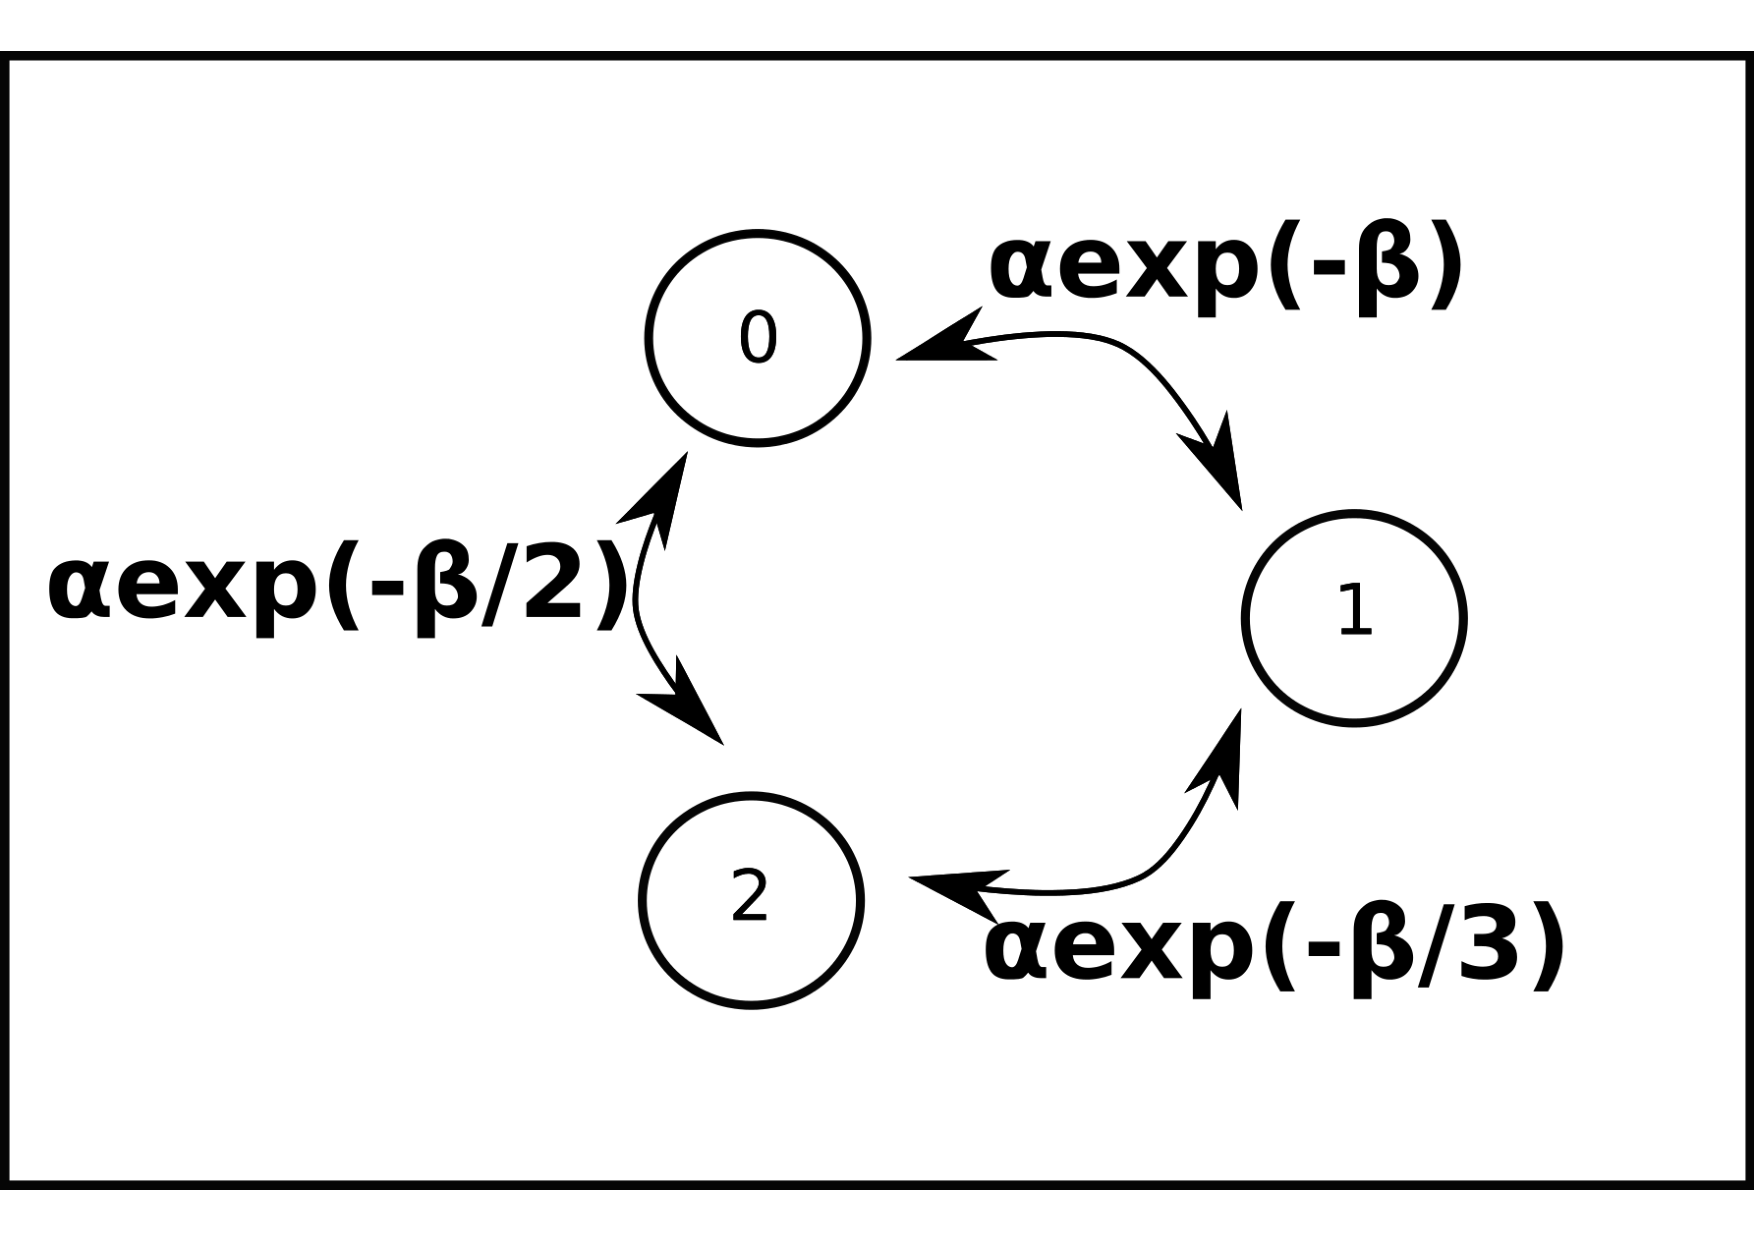
\includegraphics [width=\textwidth, angle=0]{figs/exp_model.pdf}
    \caption{A 3-state MJP with exponentially decaying rates}
    \label{fig:exp_model}
      \end{minipage}
%    \vspace{-.1in}
  \end{wrapfigure}
Consider an MJP with two parameters $\alpha$ and $\beta$, transitions between states $i$ and $j$ having rate $\alpha \exp(-\beta/(i+j))$.
We consider three settings: $3$ states (figure~\ref{fig:exp_model}),
$5$ states, and $10$ states.
We place Gamma$(\alpha_0,\alpha_1)$, and Gamma$(\beta_0, \beta_1)$ priors on the parameters $\alpha$ and $\beta$, with $(\alpha_0,\alpha_1,\beta_0,\beta_1)$ having values $(3,2,5,2)$ respectively. 
For each run, we draw random parameters from the prior to construct a transition matrix $A$, and placing a uniform distribution over states at time $0$, simulate an MJP trajectory.
We simulate observations uniformly at integer values on the time interval $[0, 20]$. 
Each observation is Gaussian distributed with mean equal to the state
at that time, and variance equal to $1$.  
For the Metropolis-Hastings proposal, we used a lognormal distribution centered at the current parameter value, with variance $\sigma^2$ that we vary.
% \noindent Assume: $S = [S_0,S_1, ...,S_N] \;, T = [t_0(t_{start}), t_1,...,t_N, t_{N+1}(t_{end})]$, and y as observations.\\
% We consider a specific structure of rate matrix $A$. $A_{ij} = \alpha f_{ij}(\beta), \; i \neq j$. $A_{ii} = -\sum_{j \neq i} A_{ij}$. $0 \leq f_{ij} \leq 1$. Denote $F_i(\beta) = \sum_{j \neq i} f_{ij}(\beta)$.\\
% \begin{align*}
% P(s_0, S, T | \alpha, \beta) &= \pi_0(s_0)\prod_{i = 1}^N A_{S_{i - 1}S_i} \exp(- \int_{t_{start}}^{t_{end}} |A_{S(t)}| dt)\\
% &= \pi_0(s_0) \alpha^N \prod_{i = 1}^N f_{S_{i - 1}S_i} \exp(-\alpha  \sum_{i = 0}^{N} F_{S_i}(\beta)(t_{i + 1} - t_i))\\
% \end{align*} 
%\vinayak{We studied our MH sampler, for three setting of $k$}.  
% %\begin{align*}
% %P(\alpha, \beta | s_0, S, T ) \propto \alpha^N \prod_{i = 1}^N f_{S_{i - 1}S_i} \exp(-\alpha  \sum_{i = 0}^{N} F_{S_i}(\beta)(t_{i + 1} - t_i)) p_1(\alpha)p_2(\beta)\\
% %\end{align*}
% %If we assume the priors of $\alpha$, $\beta$ are $Gamma(\mu, \lambda)$, $Gamma(\omega, \theta)$, then the posterior will have a simper form as follows. 
% \begin{align*}
% P(\alpha, \beta | s_0, S, T ) = C \alpha^{\mu + N - 1}\exp(-\alpha (\lambda + \sum_{i = 0}^{N} F_{S_i}(\beta)(t_{i + 1} - t_i))) \prod_{i = 1}^N f_{S_{i - 1}S_i}  \beta ^{\omega - 1} \exp(-\theta \beta)\\
% \end{align*}
% We notice that given $\beta,\; S,\; T$, $\alpha$ is distributed as a $Gamma$ distribution.\\
% $\alpha | \beta, S, T, y  = \alpha | \beta, S, T \sim Gamma(\mu + N, \lambda + \sum_{0}^NF_{S_i}(\beta)(t_{i + 1} - t_i))$.\\
% There is no conjugate distribution to sample $\beta \sim P(\beta| s_0, S, T)$. We will have to use Metropolis Hasting within Gibbs to sample $\beta$. The target distribution is the following one.
% $$ P(\beta | S, T) = C \frac{\prod_{i = 1}^N f_{S_{i -1}S_i}(\beta)\beta^{\omega - 1} \exp(-\theta \beta)}{(\lambda + \sum_{i = 0}^{N} F_{S_i}(\beta)(t_{i + 1} - t_i))^{\mu + N}}.$$
% Such doubling might slow the mixing of the Markov chain. We can apply our Metropolis Hasting algorithm on this model.

\noindent \textbf{Results:}
Figure~\ref{fig:ESS_EXP_D10} plots the ESS per unit time for the parameters $\alpha$ (left) and $\beta$ (right) for the case of $3$ states (top row) and $10$ states (bottom row) as we vary the scale-parameter $\sigma^2$ of the log-normal proposal distribution. 
We include results for $5$ states in the appendix, the conclusions are the same. 
  %as we change the variance of the
  %proposal kernel, for different methods and different scaling parameters.
  %($\kappa =
%1.5, 2, 3$) and dimensions($p = 3, 5, 10$).
%, where   $k = 1.5$,  $\Omega(\theta, \theta^*) = k \max(\max A(\theta), \max A(\theta^*))$. 
%For particle MCMC, the number of particles can be $5, 10 , 20$. 
%  Blue lines are the Gibbs sampler, orange lines are \naive\ MH, red lines 
%are the symmetrized MH and black lines are particle MCMC. 
%For methods involving standard uniformization (Gibbs and \naive\ MH), dots 
%correspond to $\kappa = 1$, triangles correspond to $\kappa = 2$, and squares 
%correspond to $\kappa = 1.5$. For our symmetrized MH algorithm, circles,
%triangles and squares correspond to $\Omega = (\Omega_{old} + \Omega_{new}),
%2(\Omega_{old} + \Omega_{new})$ and $1.5 \max(\Omega_{old}, \Omega_{new})$
%respectively, where $\Omega_{new}$ and $\Omega_{old}$ equal $\max_i A_i$ under 
%the proposed and current parameters.
%  For particle MCMC, the dot-dashed lines correspond to 
%  $5$ particles,  the dashed lines correspond to $10$ particles, and the solid 
%  lines correspond to $20$ particles.
We see that our symmetrized MH algorithm is significantly more efficient than the baselines over a wide range of choices of $\sigma^2$, (including the natural choice of $1$).
Among the three setting of our algorithm, the simple additive setting
 ({triangles}) does best, though it is only slightly better than 
 the {max-of-max} setting (circles). 
 {A reason for this improvement is that the additive setting is more stable than the max-of-max setting, when the proposal variance can be large. 
   The {additive setting with a multiplicative factor of $1.5$} (squares) does worse than both {additive choice with smaller multiplicative factor and the max-of-max choice} but still better than the other algorithms. 
   Among the baselines, simple Gibbs sampling does better than \naive\ Metropolis-Hastings, suggesting that the dependency of the Poisson grid on the MJP parameters does indeed significantly slow down mixing. 
   Particle MCMC has the worst performance for this task. 
   The results in figure~\ref{fig:ESS_EXP_D10} for the 10-dimensional state space show that for the parameter $\alpha$, the improvement that our proposed sampler affords is even more dramatic. 
   For the parameter $\beta$ however, performance is comparable to Gibbs, %although it is not possible to claim one is 
   with neither uniformly superior to the other.
  \begin{figure}[H]
%    \vspace{-.2in}
  \centering
  \begin{minipage}[!hp]{0.99\linewidth}
  \centering
  \begin{minipage}[!hp]{0.99\linewidth}
    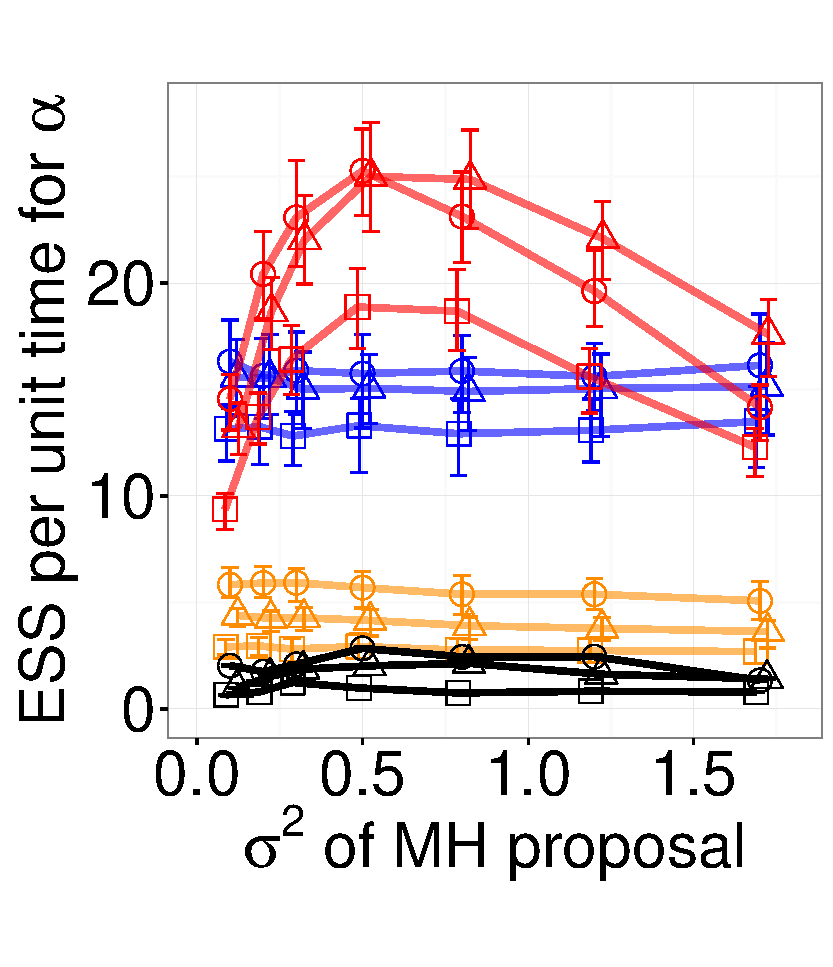
\includegraphics [width=0.45\textwidth, angle=0]{figs/exp_3_alpha.pdf}
    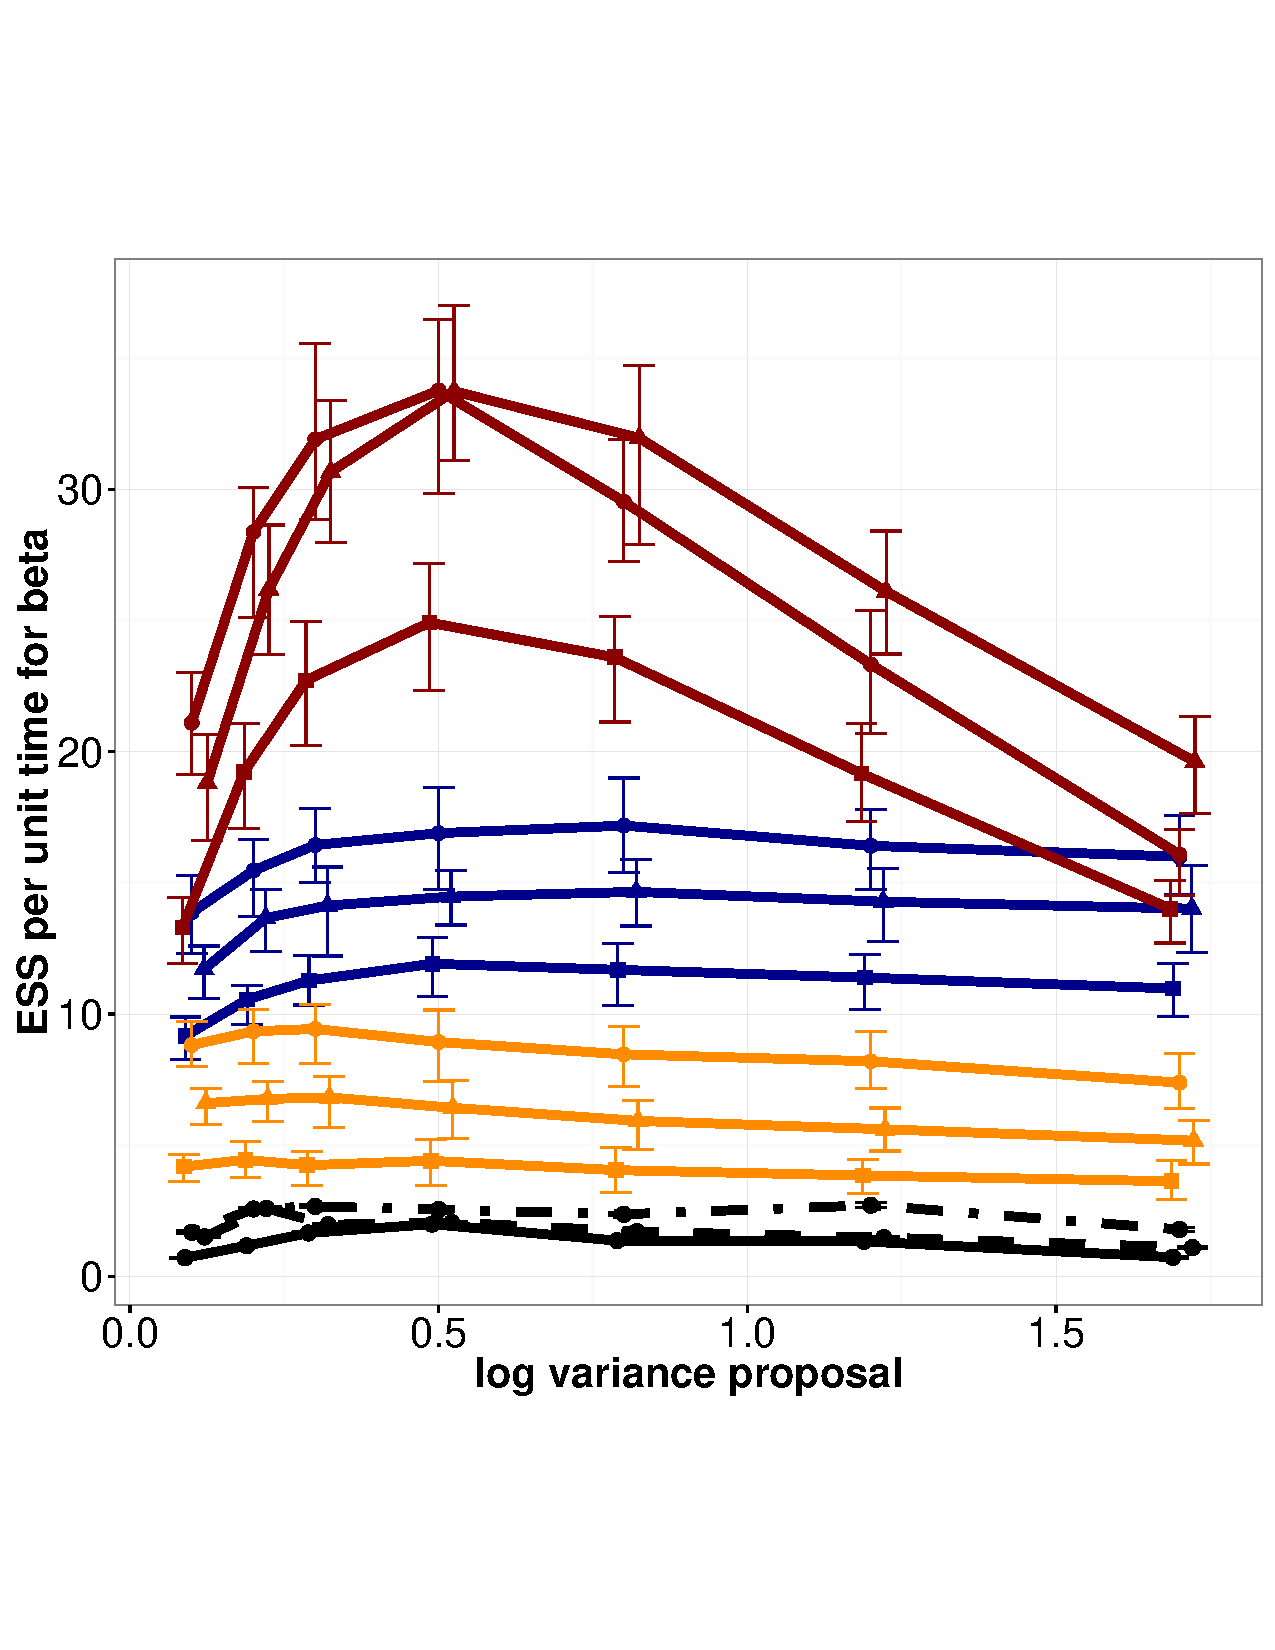
\includegraphics [width=0.45\textwidth, angle=0]{figs/exp_3_beta.pdf}
  \end{minipage}
  \centering
%   \vspace{-.3in}
  \begin{minipage}[!hp]{0.99\linewidth}
    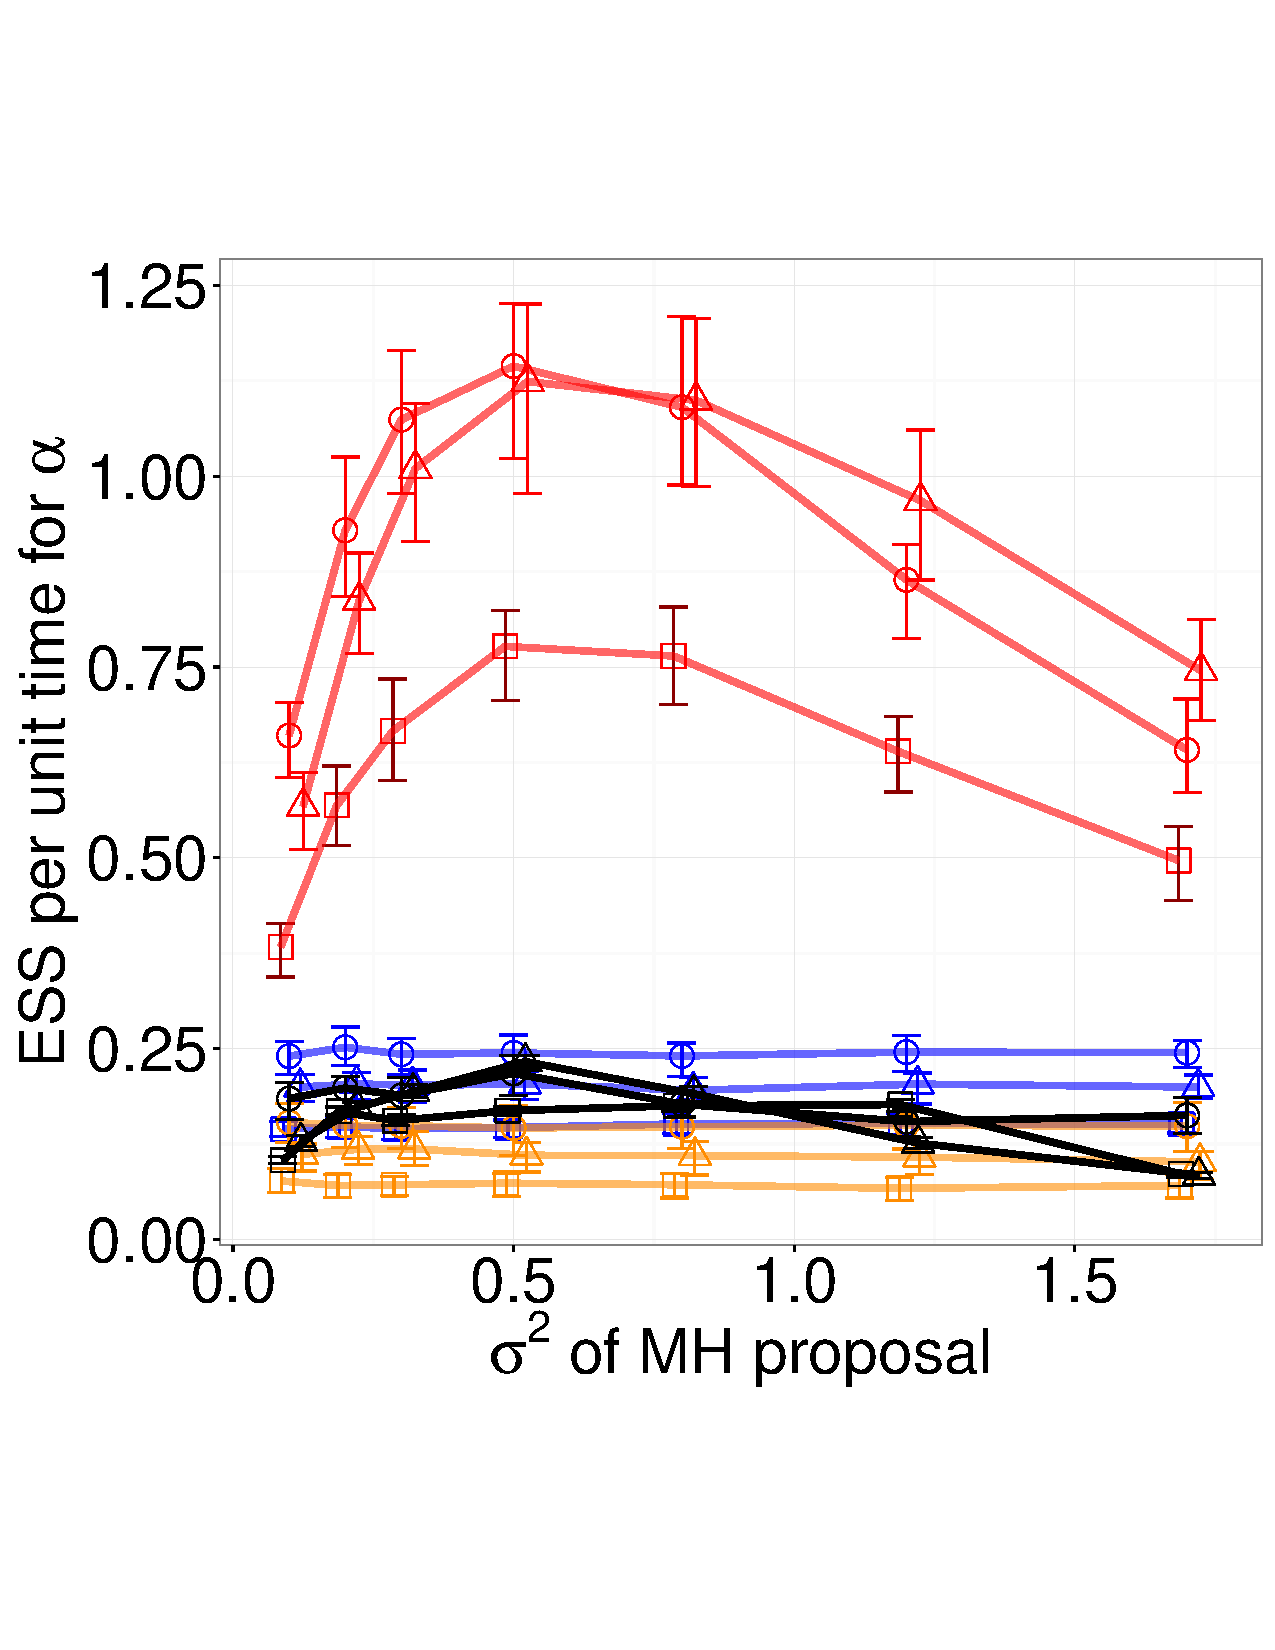
\includegraphics [width=0.45\textwidth, angle=0]{figs/exp_10_alpha.pdf}
    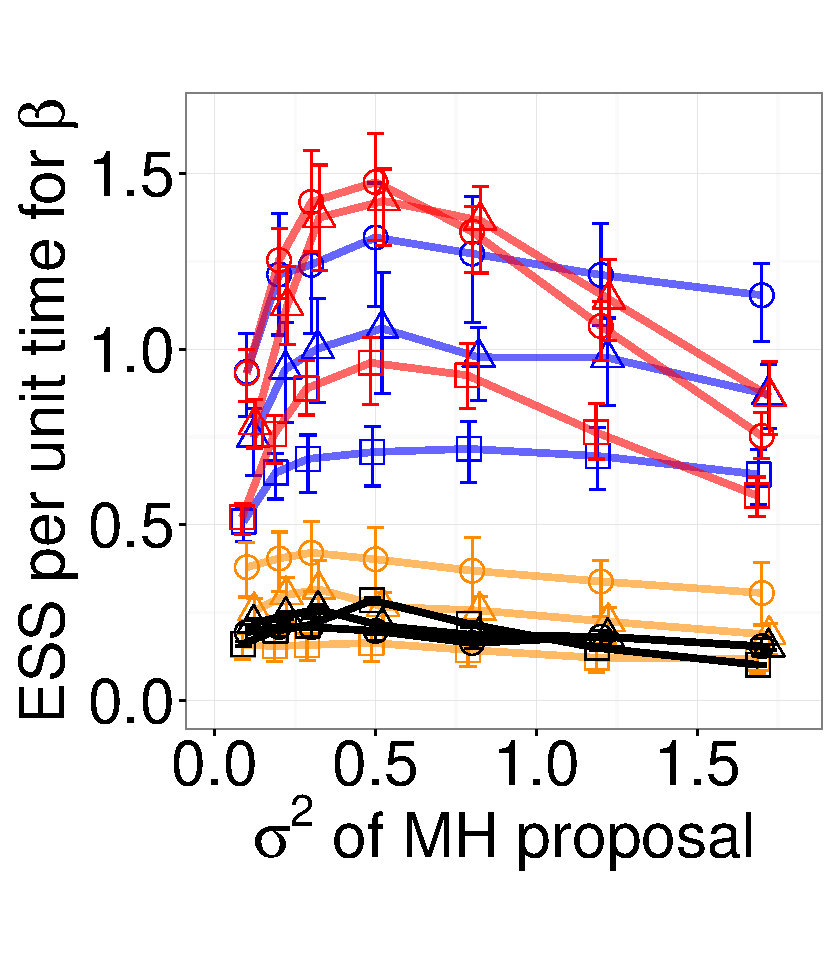
\includegraphics [width=0.45\textwidth, angle=0]{figs/exp_10_beta.pdf}
  \end{minipage}
  \end{minipage}
%  \begin{minipage}[!hp]{0.99\linewidth}
    \caption{ESS/sec for the synthetic  model, the top row being dimension 3, and the bottom,
      dimension 10. The left column is for $\alpha$, and the 
    right is for $\beta$. Red, yellow, blue and black curves are the symmetrized MH,
  \naive\ MH, Gibbs and particle MCMC algorithm. Different symbols correspond
to different settings of the algorithms, see section~\ref{sec:expts}}
     \label{fig:ESS_EXP_D10}
%  \end{minipage}
  \end{figure}

  \begin{figure}[H]
%    \vspace{-.2in}
  \centering

  \begin{minipage}[!hp]{0.99\linewidth}
    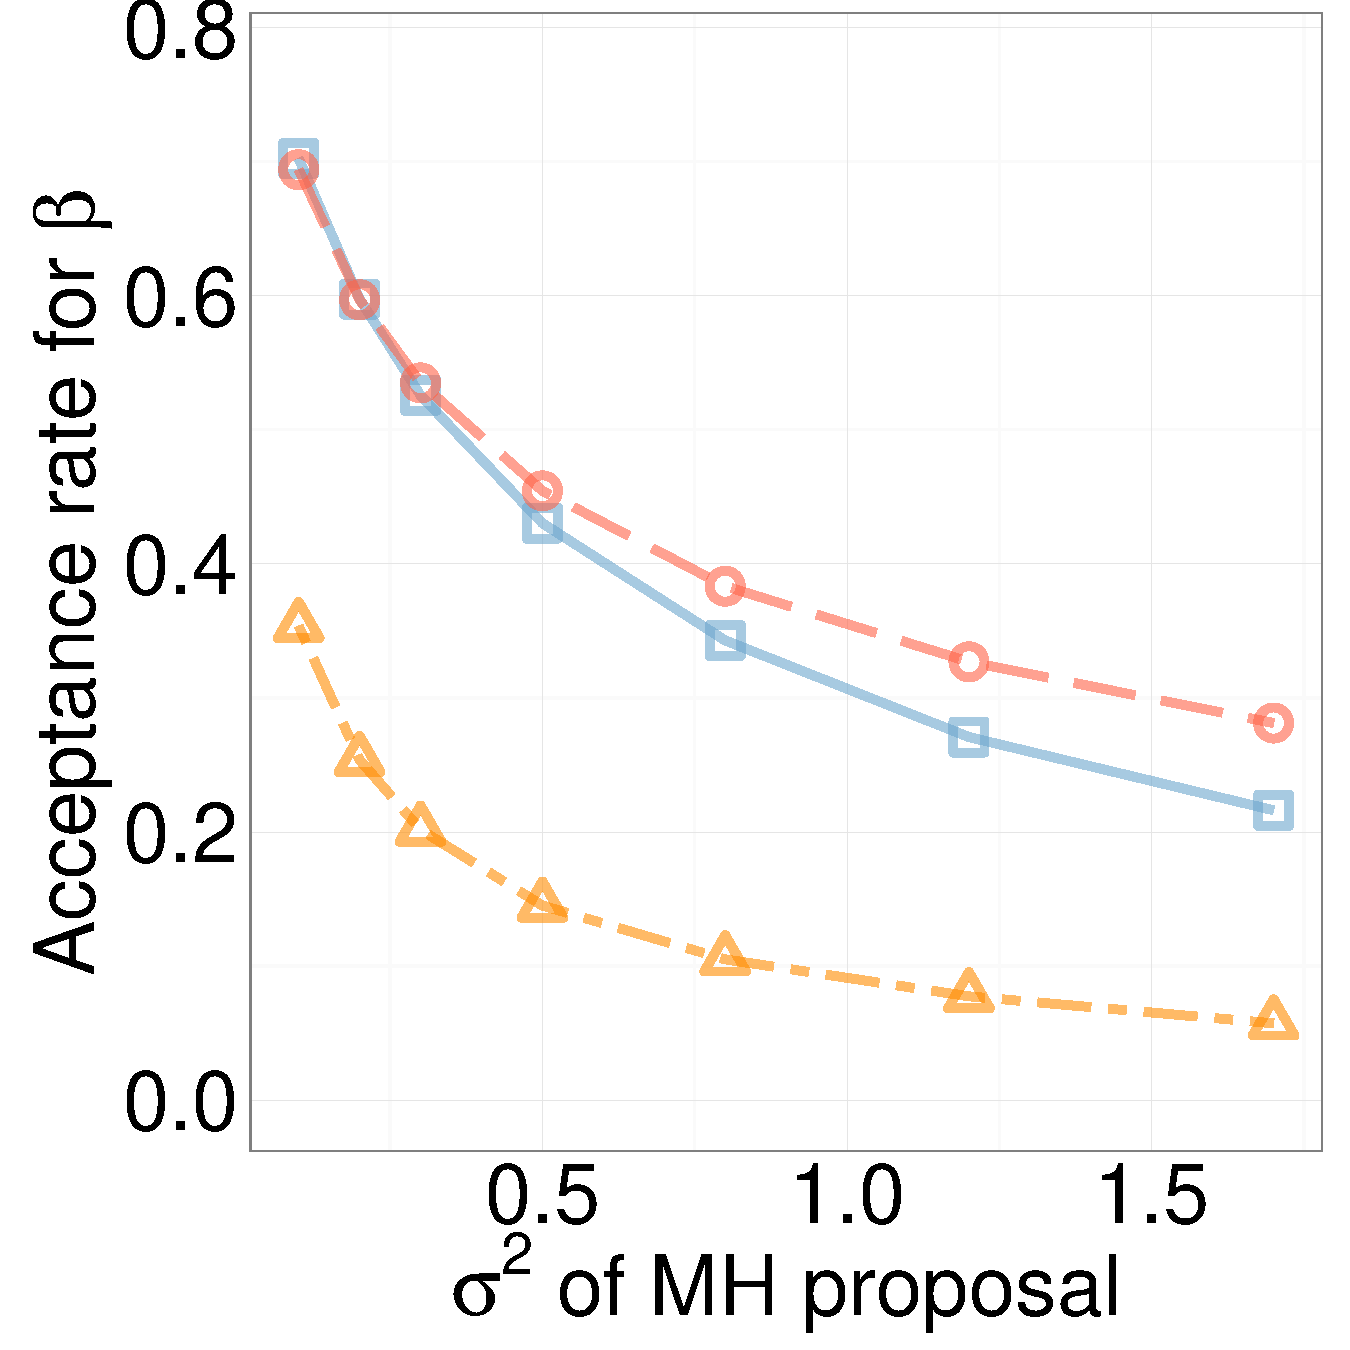
\includegraphics [width=0.40\textwidth, angle=0]{figs/acc/EXP_D3beta_k2.pdf}
	\hspace{.5in}
    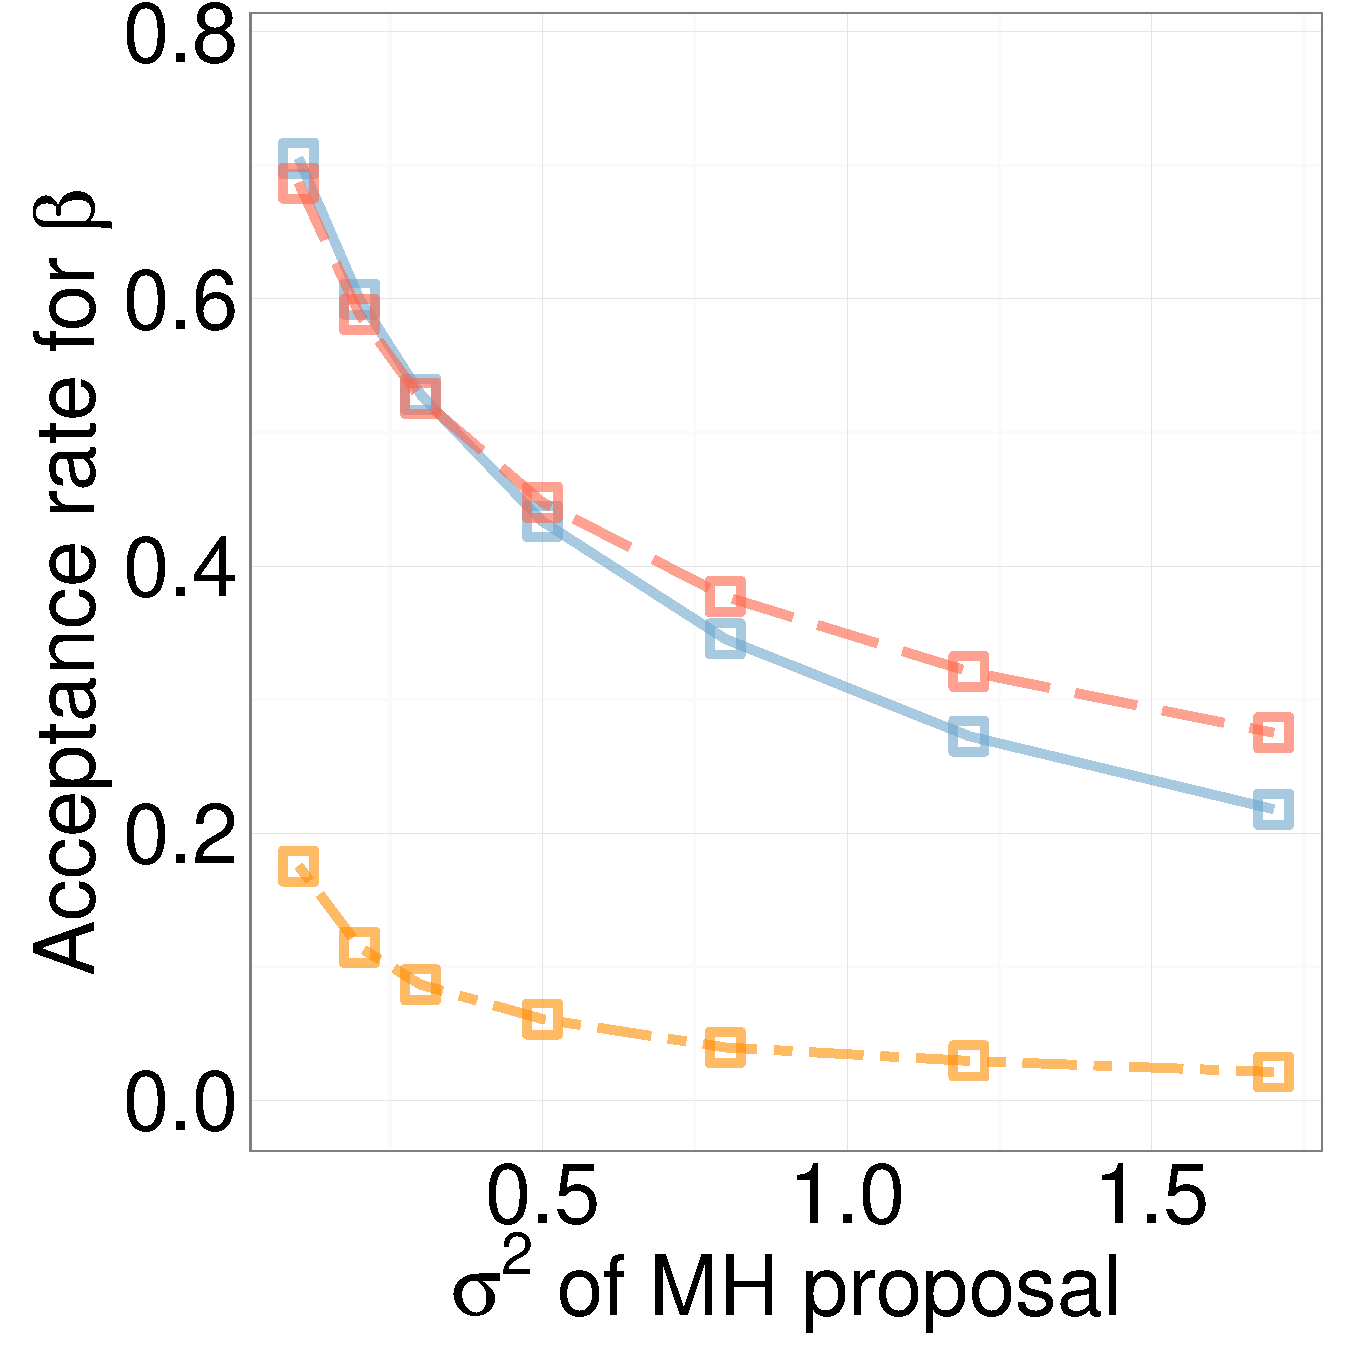
\includegraphics [width=0.40\textwidth, angle=0]{figs/acc/EXP_D10beta_k2.pdf}
  \end{minipage}
%  \begin{minipage}[!hp]{0.99\linewidth}
    \caption{Acceptance Rate for $\beta$ in the synthetic model, the left row being dimension 3, and the right,dimension 10.  Red, yellow and blue curves are the Gibbs, symmetrized MH,
 and \naive\ MH  algorithm. The multiplicative factor is $2$. }
     \label{fig:ACC_EXP}
%  \end{minipage}
  \end{figure}

%  \begin{figure}[H]
%    \vspace{-.2in}
%  \centering
 % \begin{minipage}[!hp]{0.99\linewidth}
%  \centering
 % \begin{minipage}[!hp]{0.99\linewidth}
   % 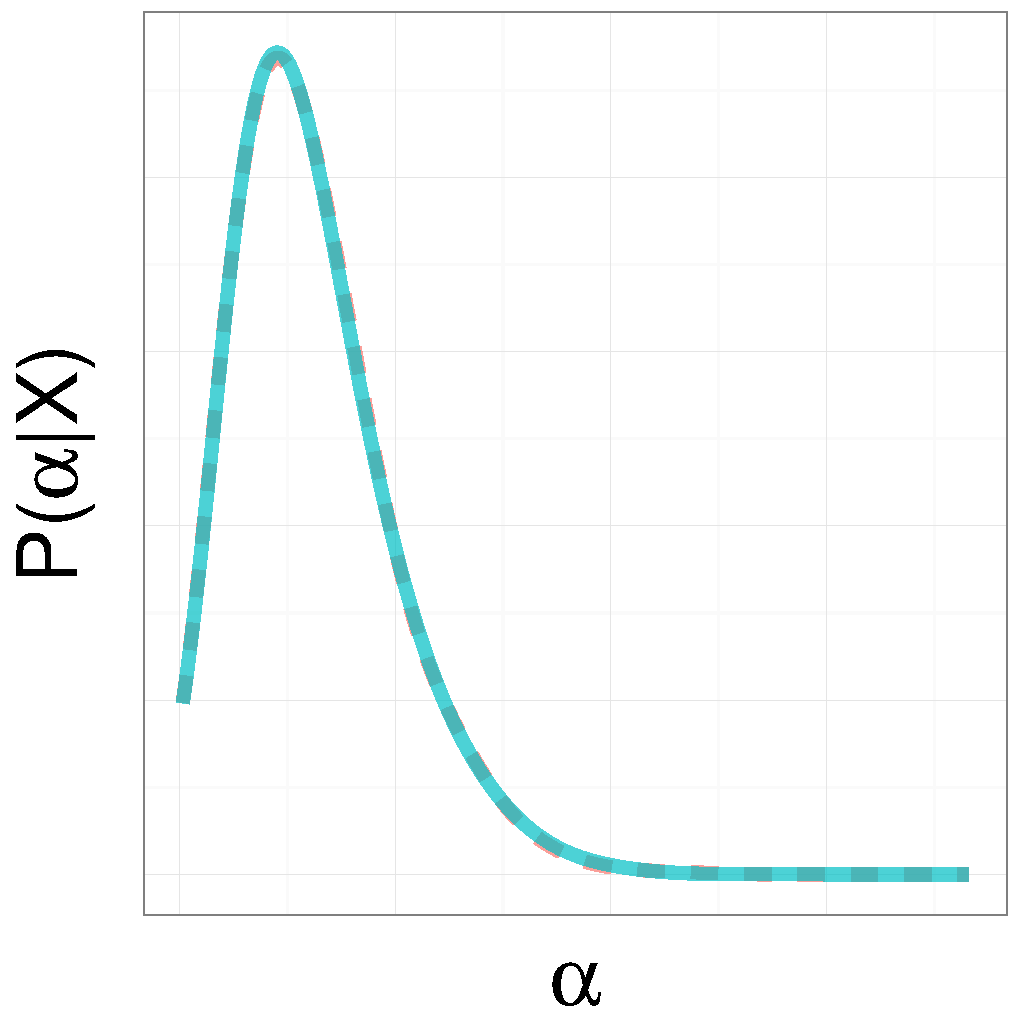
\includegraphics [width=0.45\textwidth, angle=0]{figs/EXP_ks/exp_hist_7_05_3_.pdf}
    %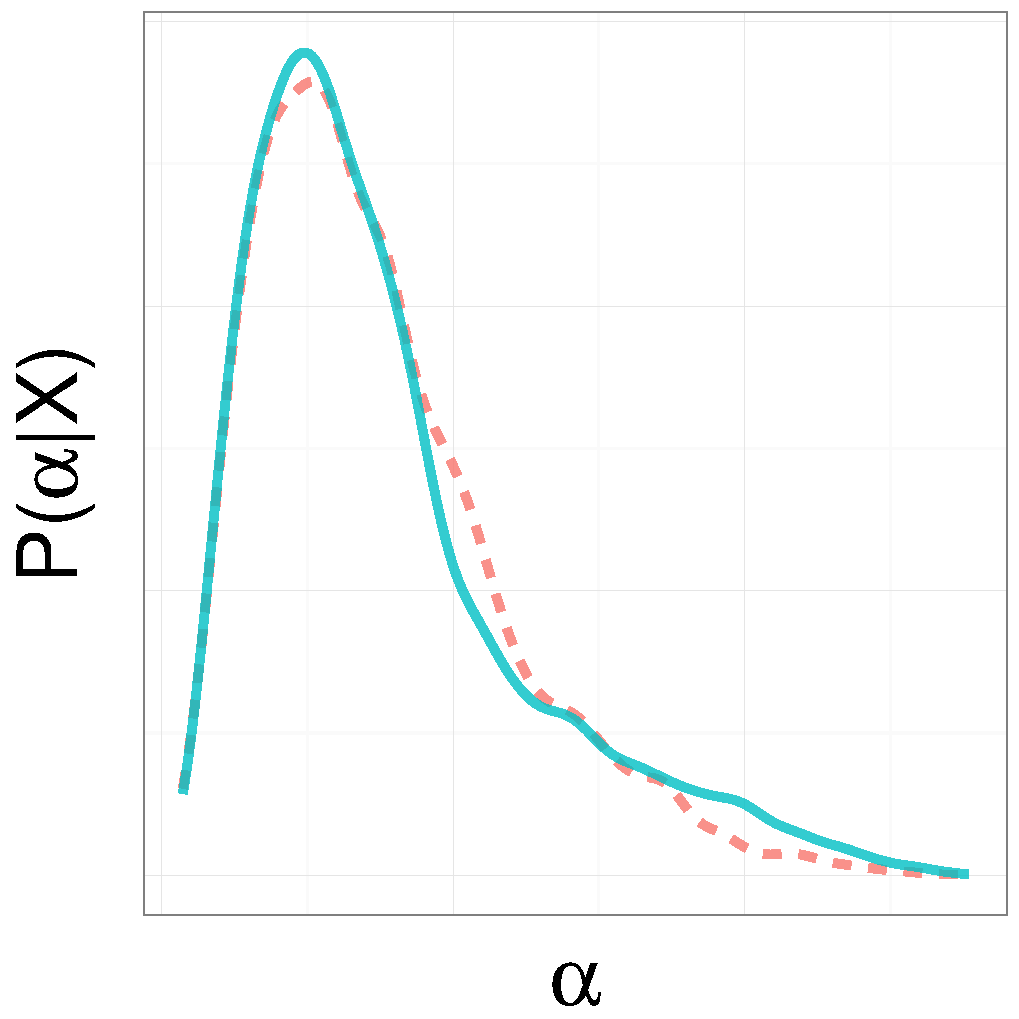
\includegraphics [width=0.45\textwidth, angle=0]{figs/EXP_ks/exp_hist_44_05_10_.pdf}
  %\end{minipage}

%  \end{minipage}
%  \begin{minipage}[!hp]{0.99\linewidth}
    %\caption{Histograms for the posterior samples of the synthetic model, the left being dimension 3 and the right being dimension 10. The red and blue curves are the Gibbs and symmetrized MH}
%     \label{fig:HIST_EXP}
%  \end{minipage}
%  \end{figure}

  \begin{figure}[H]
%    \vspace{-.2in}
  \centering
%  \begin{minipage}[!hp]{0.99\linewidth}
 % \centering
  \begin{minipage}[!hp]{0.97\linewidth}
    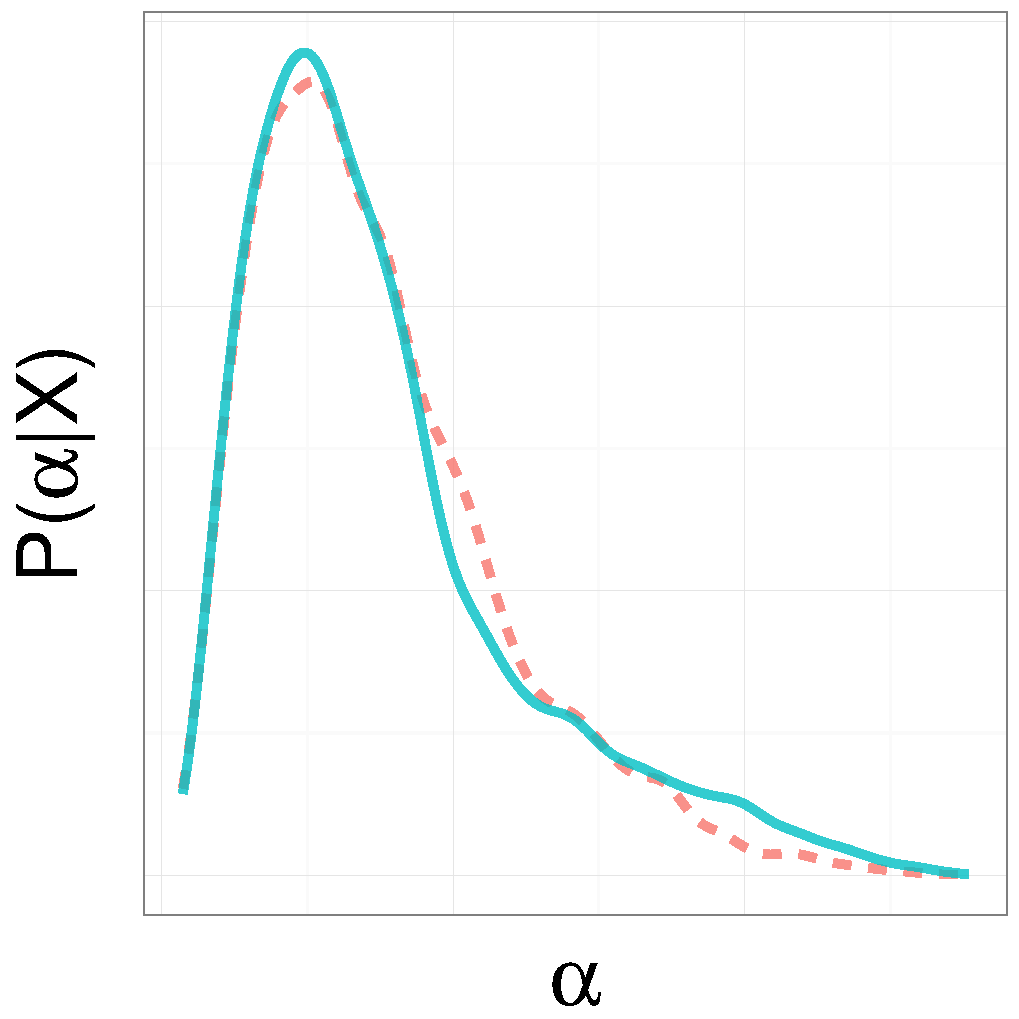
\includegraphics [width=0.30\textwidth, angle=0]{figs/EXP_ks/exp_hist_44_05_10_.pdf}
    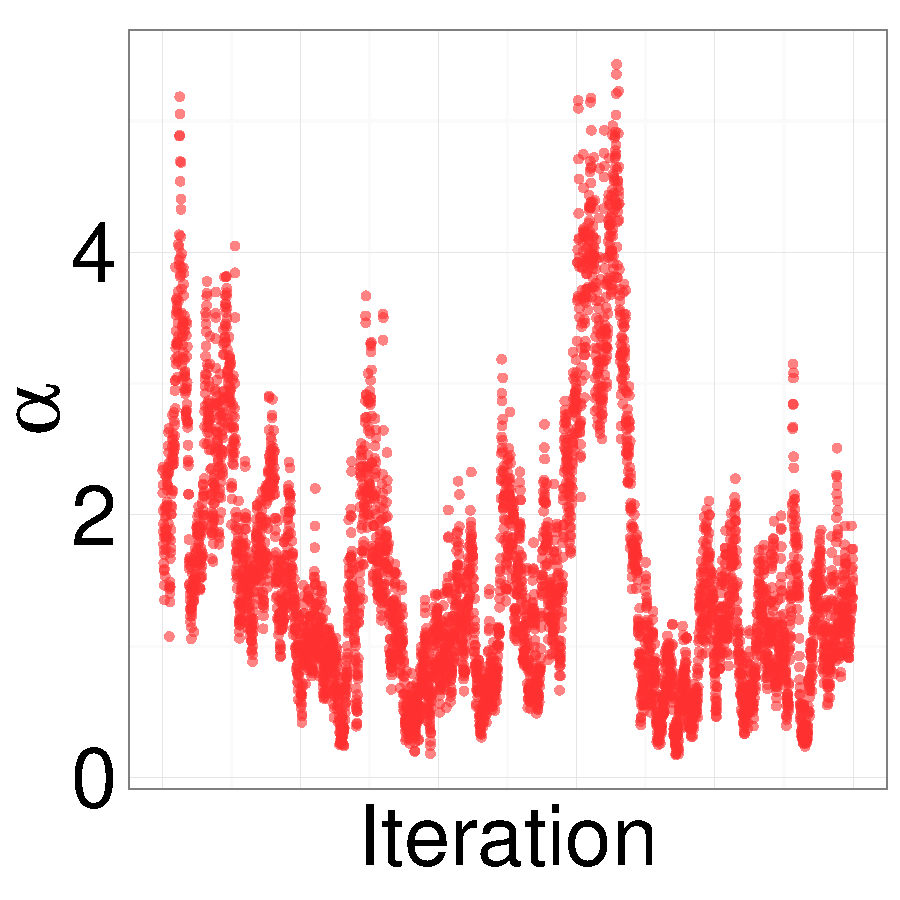
\includegraphics [width=0.30\textwidth, angle=0]{figs/EXP_ks/exp_traceGBS_44_05_10_.pdf}
    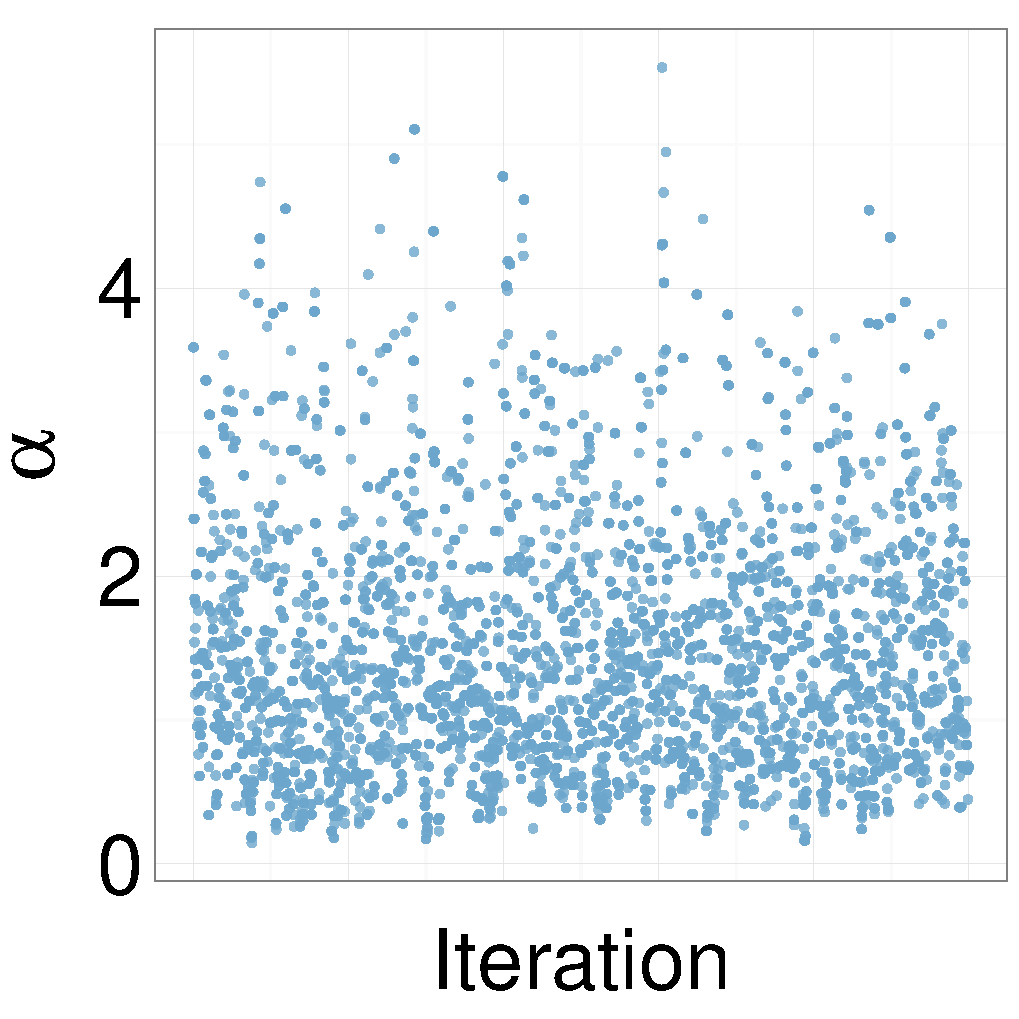
\includegraphics [width=0.30\textwidth, angle=0]{figs/EXP_ks/exp_traceMH_44_05_10_.pdf}
  \end{minipage}

%  \end{minipage}
%  \begin{minipage}[!hp]{0.99\linewidth}
    \caption{The left is histogram for the posterior samples($\alpha$) of the synthetic model, the red and blue curves are the Gibbs and symmetrized MH. The p value of the two sample-Kolmogorov Smirnov test is $0.5085$. The middle and the right are trace plots for the posterior samples of the synthetic model with dimension 10, the middle is for Gibbs and the right is for symmetrized MH}
     \label{fig:TRACE_EXP}
%  \end{minipage}
  \end{figure}

  \begin{figure}[H]
%    \vspace{-.2in}
  \centering
  \begin{minipage}[!hp]{0.99\linewidth}
    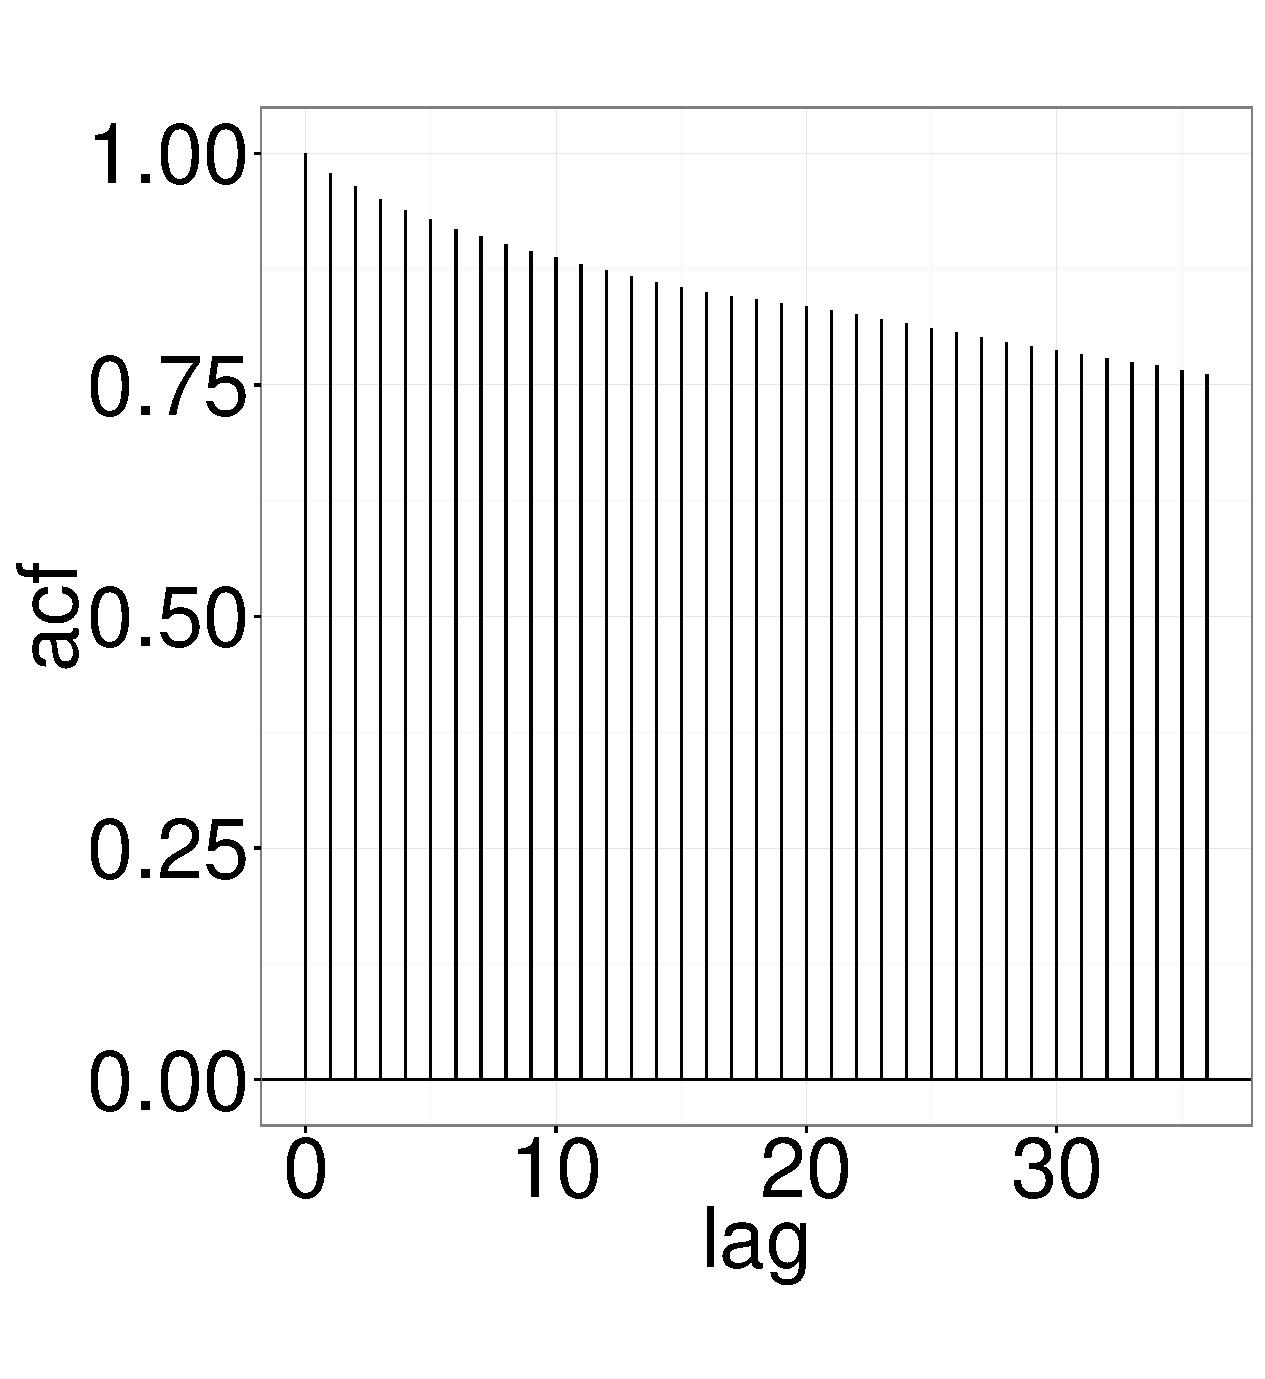
\includegraphics [width=0.40\textwidth, angle=0]{figs/EXP_ks/exp_gbsacf_44_05_10_.pdf}
	\hspace{.5in}
    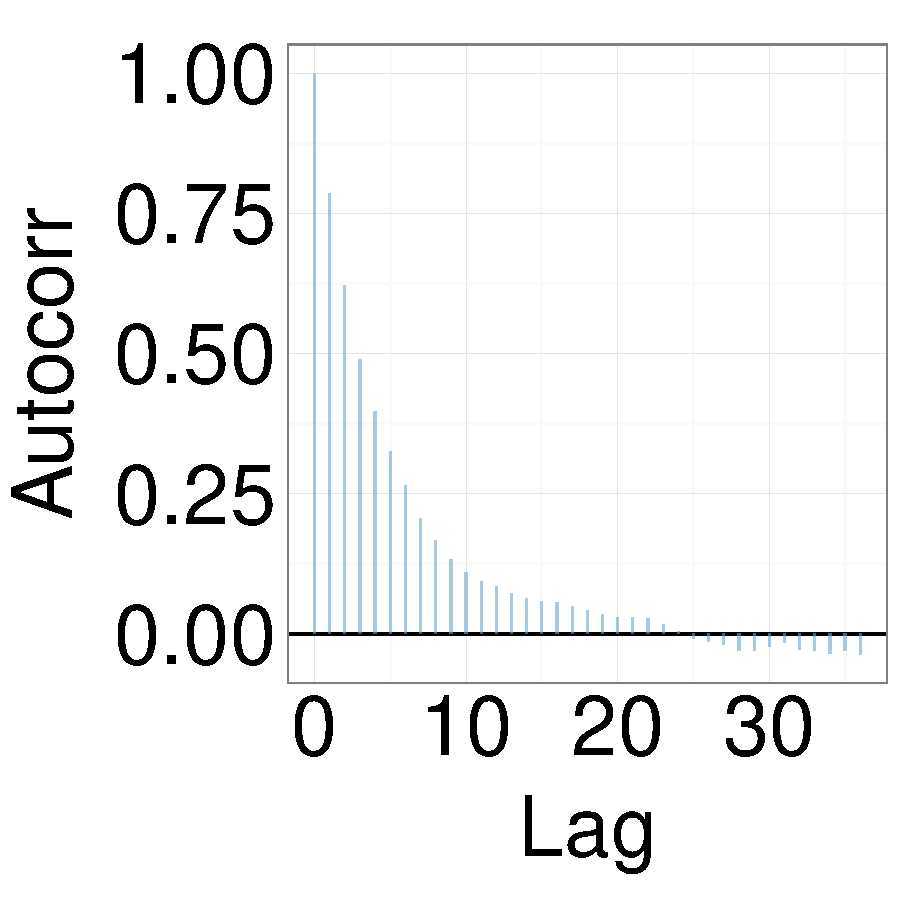
\includegraphics [width=0.40\textwidth, angle=0]{figs/EXP_ks/exp_mhacf_44_05_10_.pdf}
  \end{minipage}

%  \begin{minipage}[!hp]{0.99\linewidth}
    \caption{ACFs for the posterior samples $\alpha$ of the synthetic model with dimension 10. The left is for Gibbs, and the right is for symmetrized MH.}
     \label{fig:ACF_EXP}
%  \end{minipage}
  \end{figure}

  \begin{figure}%[b]    
  \centering
  \begin{minipage}[hp]{0.24\linewidth}
  \centering
    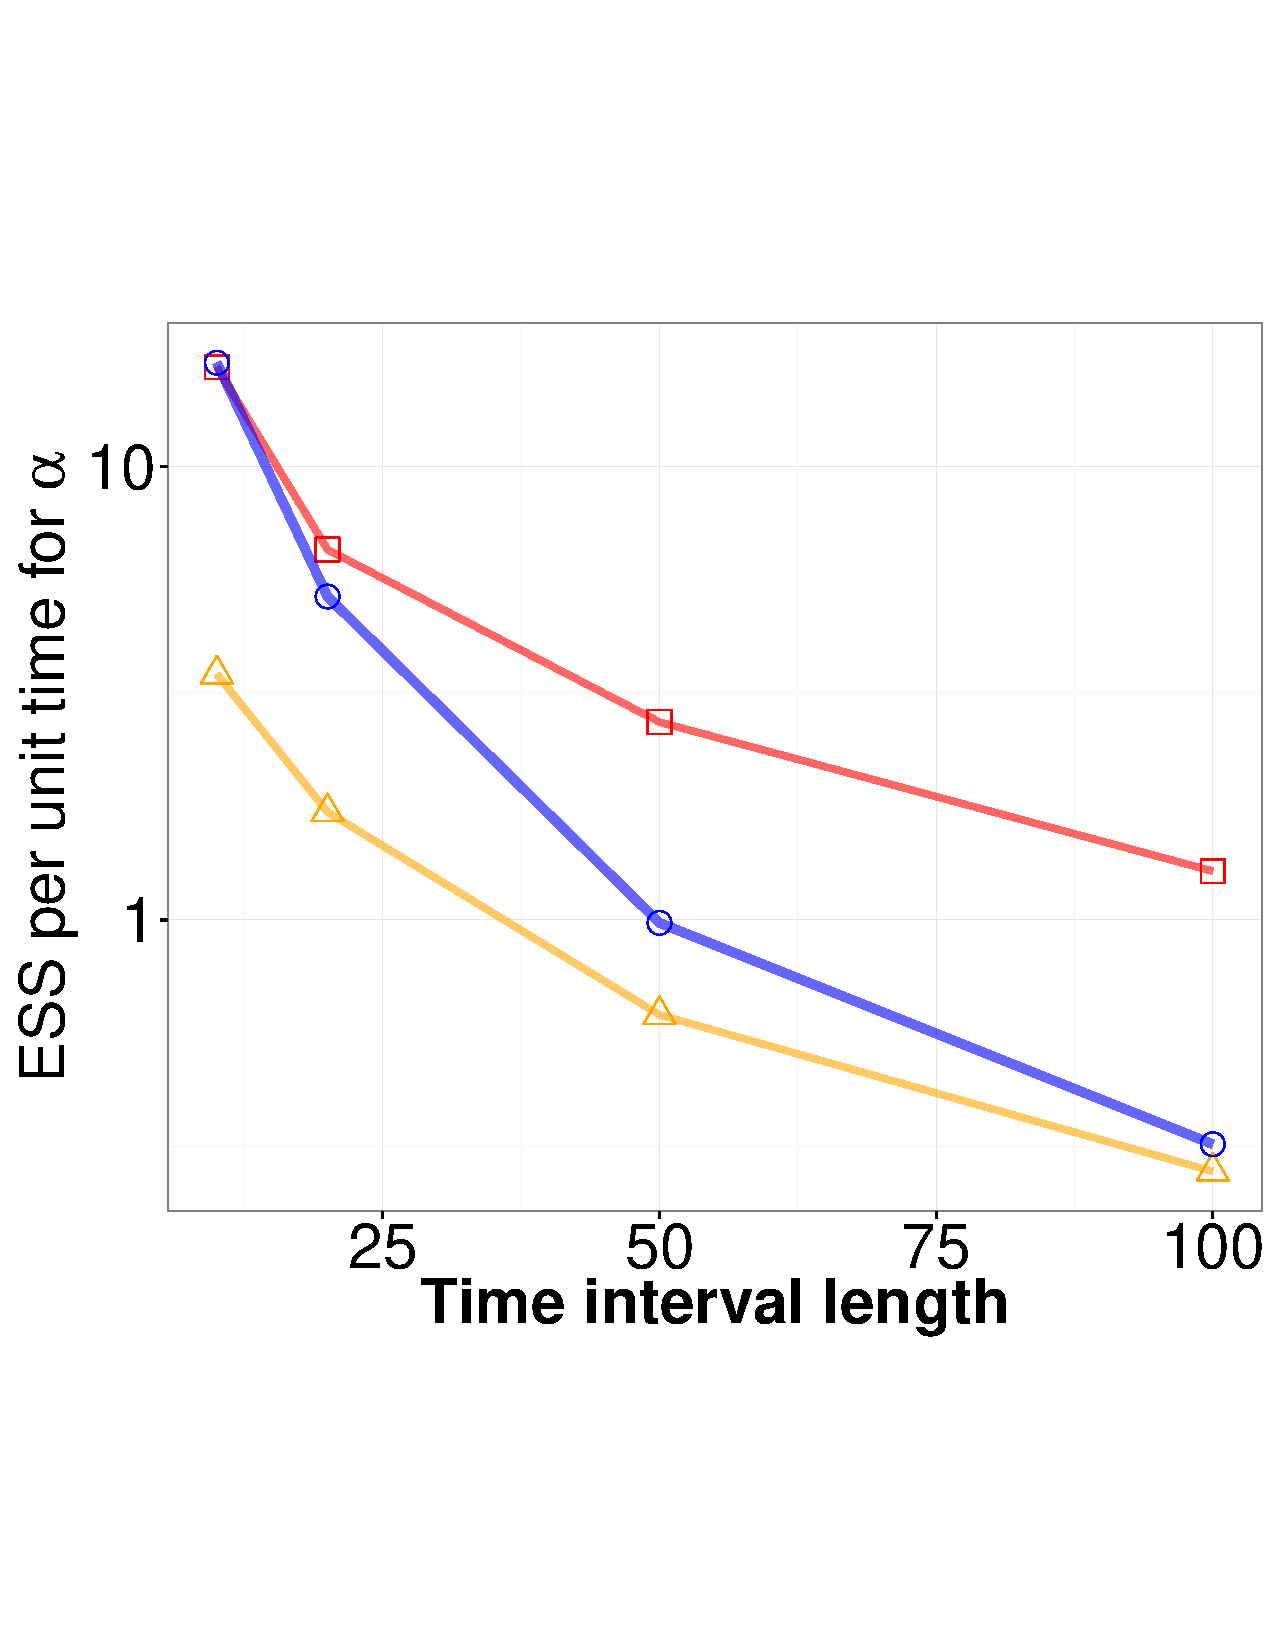
\includegraphics [width=0.99\textwidth, angle=0]{figs/ESS_vs_t_alpha_fixobservation.pdf}
    \end{minipage}
  \begin{minipage}[hp]{0.24\linewidth}
  \centering
    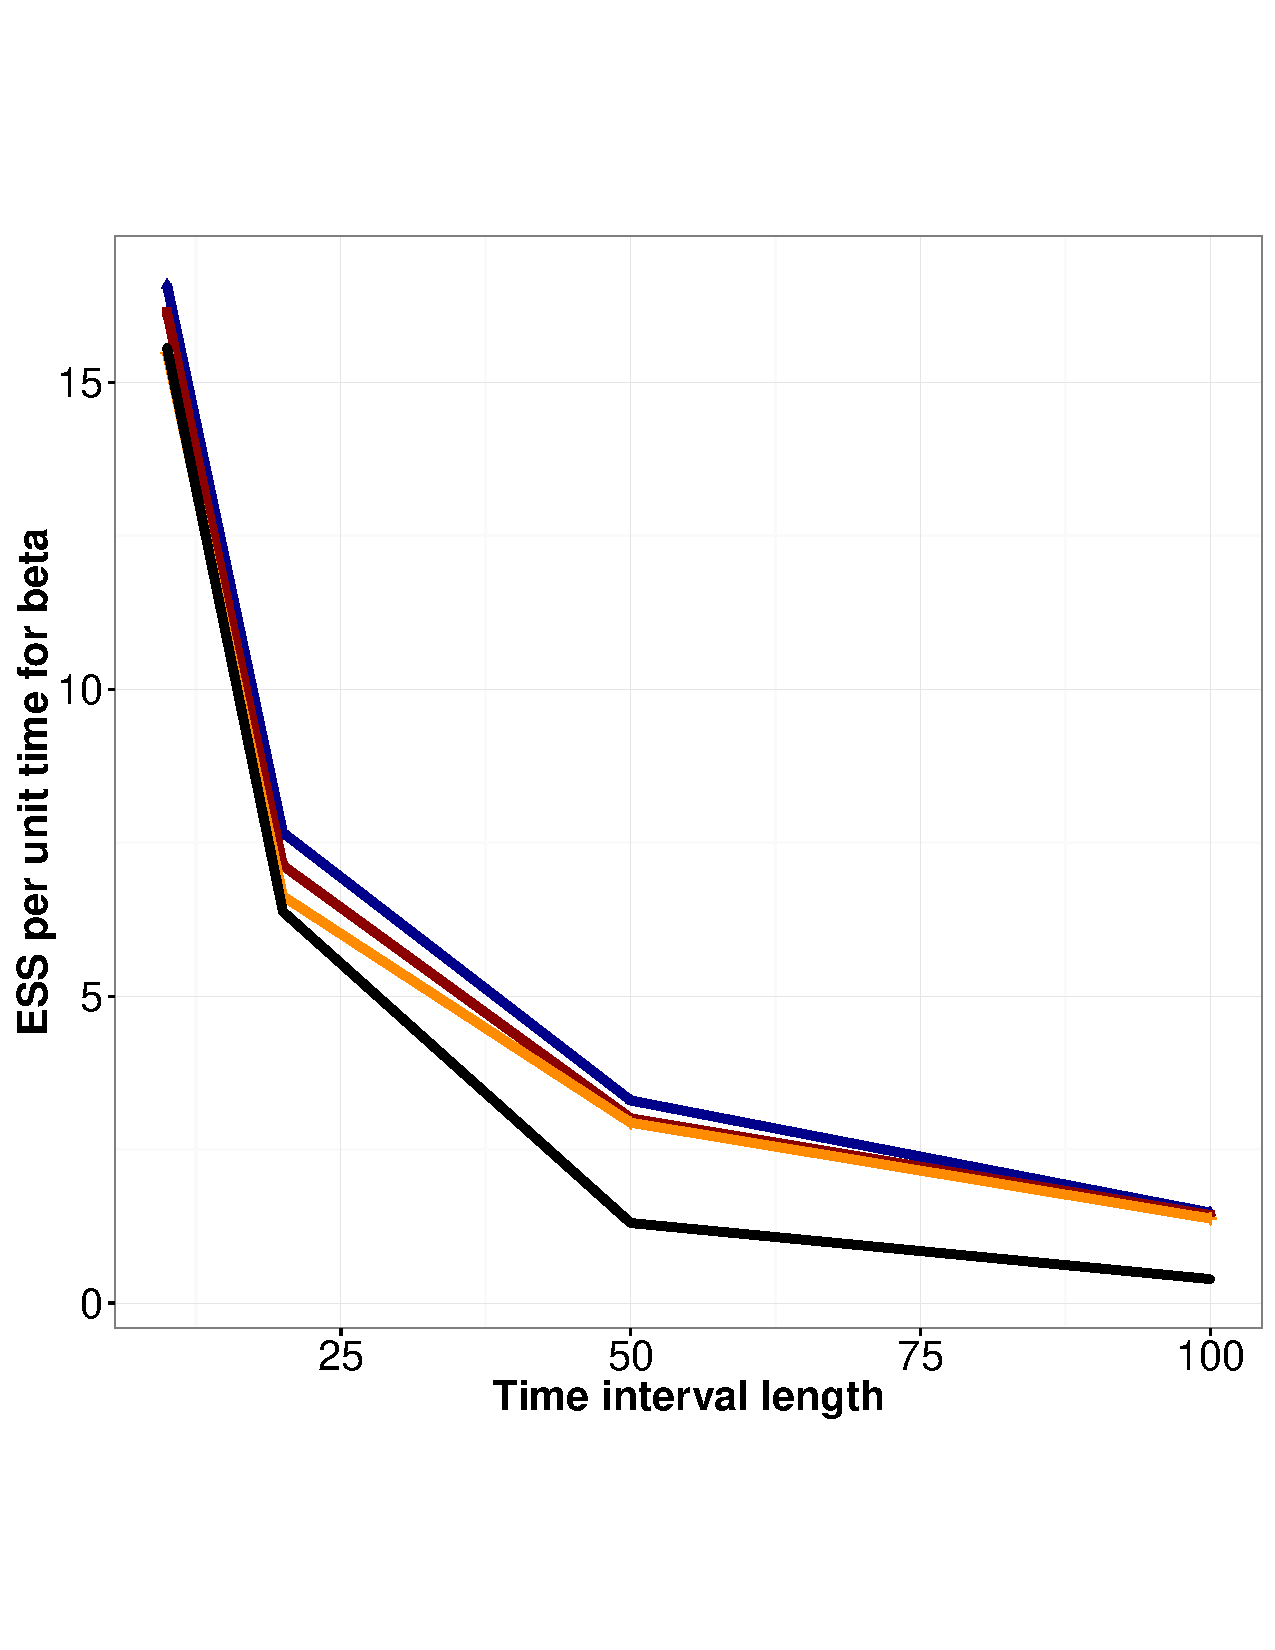
\includegraphics [width=0.99\textwidth, angle=0]{figs/ESS_vs_t_beta_fixobservation.pdf}
%    \vspace{-0.3in}
  \end{minipage}
    %\label{fig:TSS_fix}
  \begin{minipage}[hp]{0.24\linewidth}
  \centering
    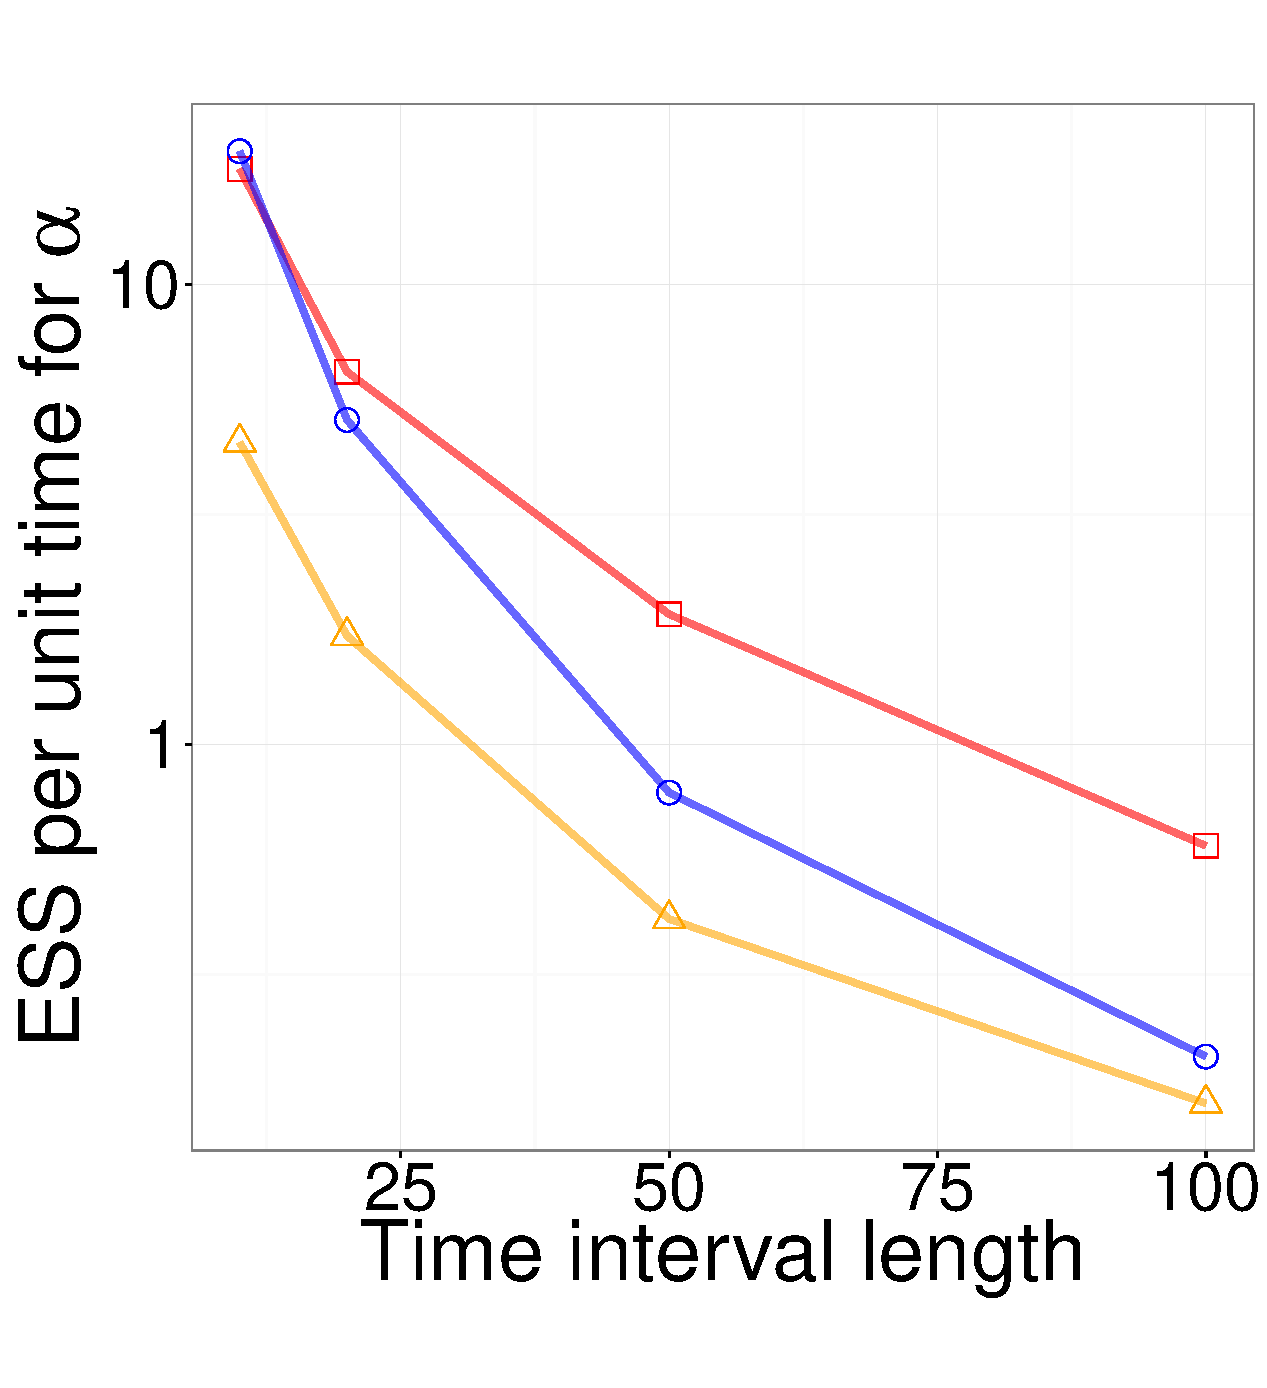
\includegraphics [width=0.99\textwidth, angle=0]{figs/ESS_vs_t_alpha.pdf}
      \end{minipage}
  \begin{minipage}[hp]{0.24\linewidth}
  \centering
    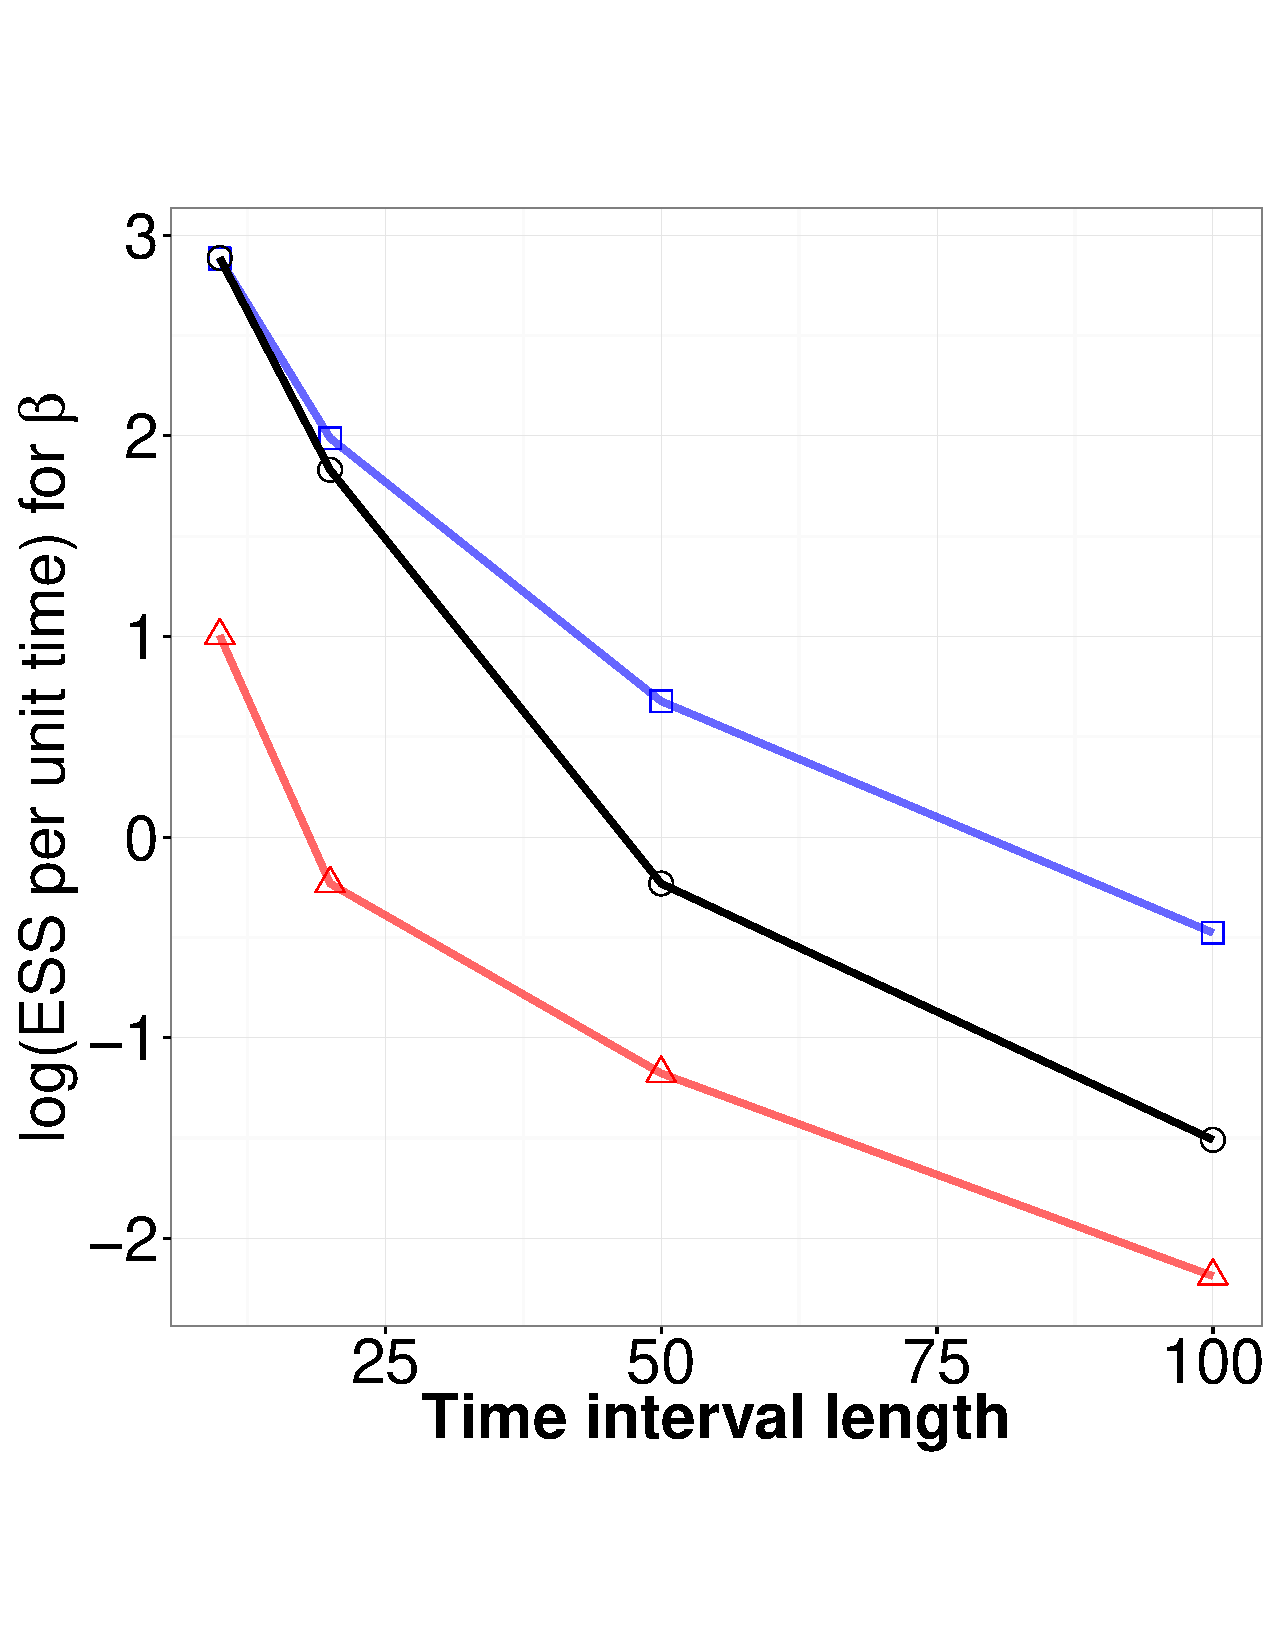
\includegraphics [width=0.99\textwidth, angle=0]{figs/ESS_vs_t_beta.pdf}
  \end{minipage}
%    \vspace{-0.3in}
%    \caption{Time Interval vs. ESS / sec}
    \caption{Time Interval vs. ESS/sec. In the left two plots, the number of 
    observations is fixed, in the right two, this grows linearly with the
    interval length. Red (square), yellow (triangle) and blue (circle) 
    curves are the symmetrized MH,
  \naive\ MH and Gibbs algorithm.}
     \label{fig:TSS}
  \end{figure}
%We generate different observations on different time intervals.
%Our observation process was a Gaussian distribution with mean equal to the 
%current state and variance equal to $1$. 
In figure~\ref{fig:TSS}, we plot ESS per unit time as the observation 
interval $t_{end}$ increases. We consider the three-state MJP, and as before there 
are $19$ observations uniformly located over a time interval $(0,t_{end})$. We 
consider four settings, with $t_{end}$ equal to $10, 20, 50, 100$. For each, we 
compare our symmetrized MH sampler (with $\kappa$ set to $1$) with the Gibbs 
sampler (with $\kappa$ set to $2$). While the performance of the Gibbs sampler 
is comparable with our symmetrized algorithm for the smallest value of 
$t_{end}$, its performance is considerably worse for longer time-intervals. 
This is because the Gibbs sampler updates $\theta$ conditioned on the MJP
trajectory, and longer time intervals result in stronger coupling 
between MJP path and parameters, and thus poorer mixing. This effect 
disappears if we integrate out the MJP trajectory. This experiment 
demonstrates that it is not sufficient just to integrate out the state 
values of the trajectory, we also have to get around the effect 
of the trajectory transition times. Our symmetrized MH-algorithm allows 
this. 
%as a by-product, it also involves calculating a simpler 
%MH acceptance probability.


To the right of figure~\ref{fig:TSS}, we plot results from a similar experiment. Now,
instead of keeping the number of measurements fixed as we increase the 
observation interval, we keep the observation rate fixed at one observation 
every unit interval of time, so that longer observation intervals have larger 
number of observations. The results are similar to the previous case: Gibbs 
sampling performs well for small observation intervals, with performance 
degrading sharply for larger intervals. These two experiments 
illustrate the importance of integrating out the MJP path while 
carrying out parameter inference.

%\vspace{-.23in}
  \subsection{The Jukes and Cantor (JC69) model}~
  \begin{figure}%[H]
%  \begin{minipage}[!hp]{0.7\linewidth}
  \begin{minipage}[!hp]{0.99\linewidth}
    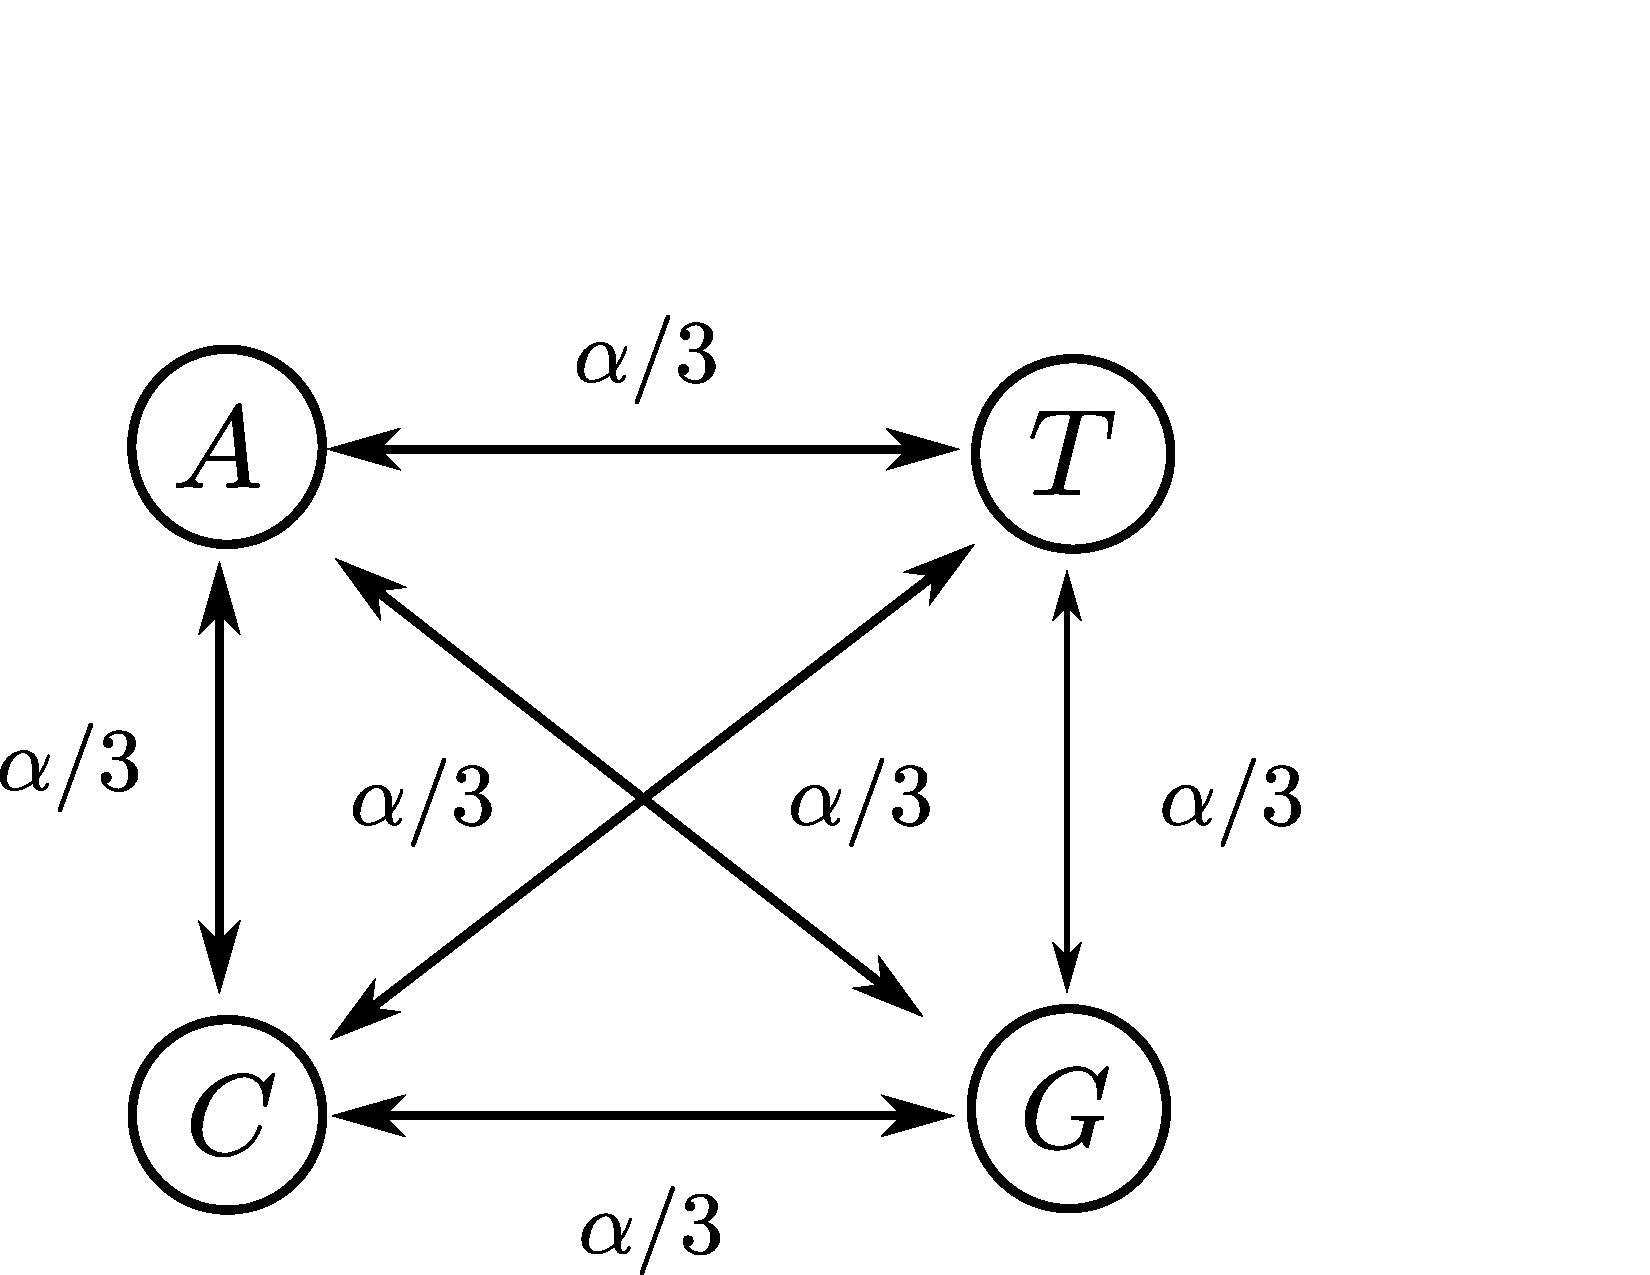
\includegraphics[width=0.40\textwidth, angle=0]{figs/jc_model.pdf}
	\hspace{.5in}
    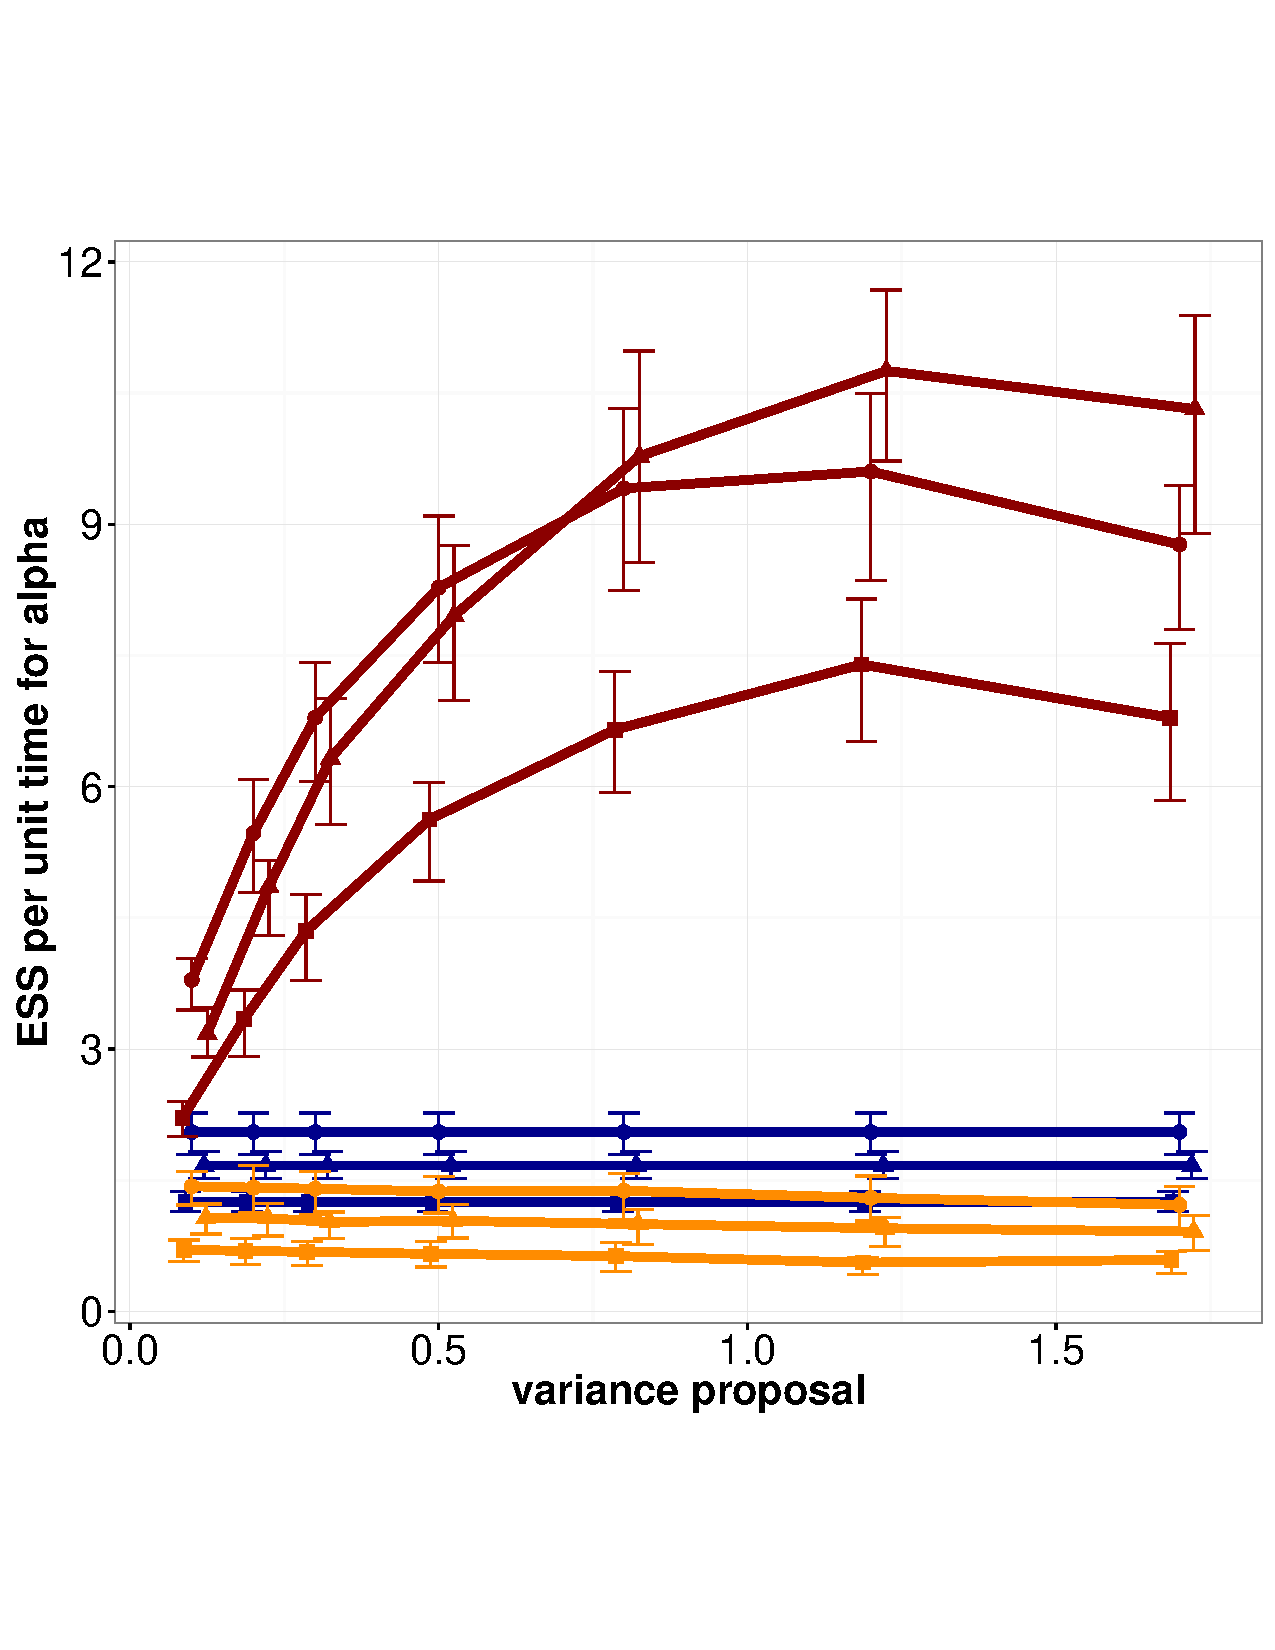
\includegraphics[width=0.40\textwidth, angle=0]{figs/jc.pdf}
	%\label{jc_model}
  \end{minipage}
%  \begin{minipage}[!hp]{0.28\linewidth}
  \caption{(a) Jukes-Cantor (JC69) model, (b)
    ESS/sec for the JC69 Model. Red, yellow and blue curves are the 
      symmetrized MH, \naive\ MH and Gibbs algorithm. }
     \label{fig:ESS_JC}
 % \end{minipage}
%\vspace{-.2in}
  \end{figure}
  The Jukes and Cantor (JC69) model~\citep{jukescantor69} is a popular model of DNA nucleotide
  substitution.  We write its state space as $\{0, 1, 2, 3\}$, representing the 
  four nucleotides $\{A, T, C, G\}$.  The model has a single parameter $\alpha$, 
  representing the rate at which the system transitions between any pair of 
  states. Thus, the rate matrix $A$ is given by 
  %Assume: $S = [S_0,S_1, ...,S_N] \;, T = [t_0(t_{start}), t_1,...,t_N, t_{N+1}(t_{end})]$, and y as observations.\\
$A_i = -A_{i,i} = 3\alpha, A_{i, j} = \alpha,i \neq j.$
We place a Gamma$(3,2)$ prior on the parameter $\alpha$.
Figure~\ref{fig:ESS_JC}(right) compares different samplers: we see that the
symmetrized MH samplers comprehensively outperforms all others.
Part of the reason why the difference is so dramatic here is because the
transition matrix is no longer sparse in this example, implying a stronger
coupling between MJP path and parameter $\alpha$. We point out that for Gibbs
sampling, the conditional parameter update is conjugate, and there is no
proposal distribution involved (hence its performance remains fixed along
the x-axis). Particle MCMC performs worse
than all the algorithms, and we do not include it in our plots.
  \begin{figure}%[H]
  \centering
%  \begin{minipage}[!hp]{0.58\linewidth}
  \begin{minipage}[!hp]{0.99\linewidth}
  \centering
    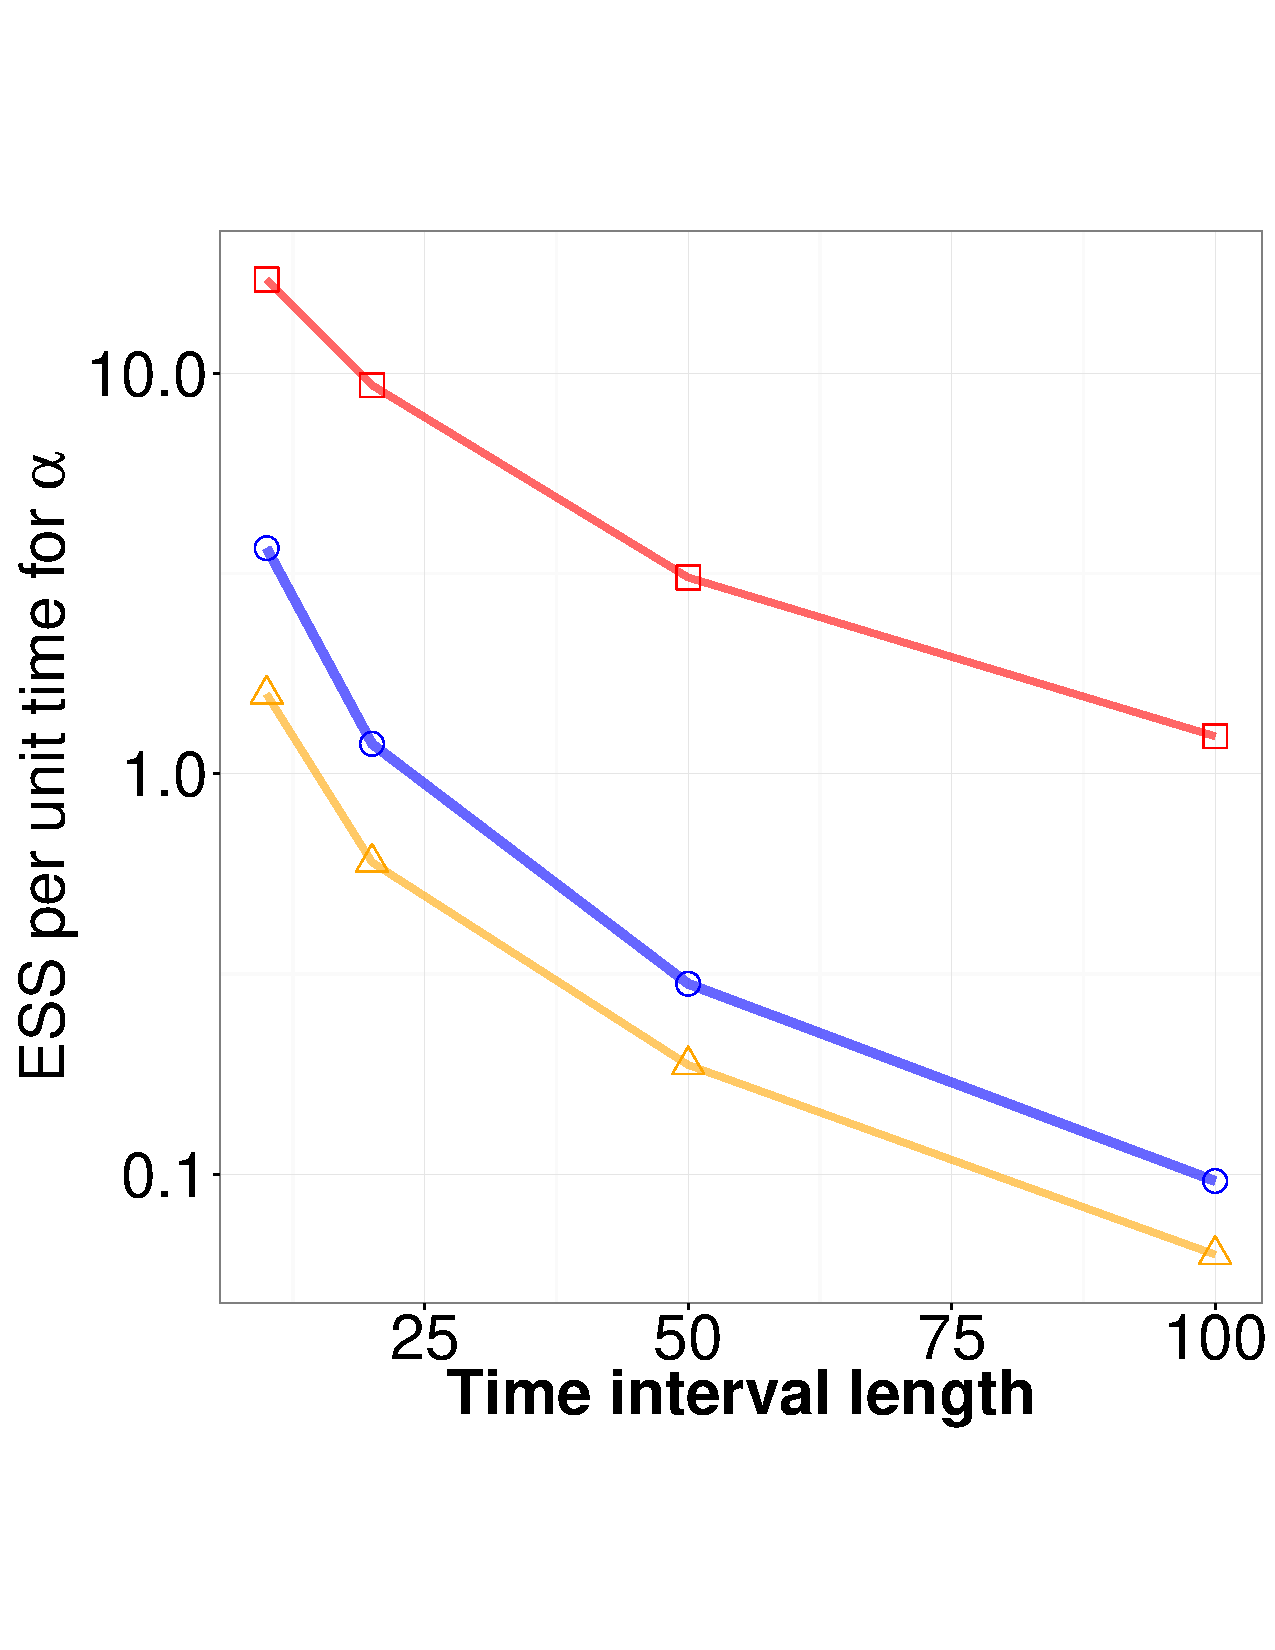
\includegraphics [width=0.40\textwidth, angle=0]{figs/ESS_vs_t_alpha_JC.pdf}
	\hspace{.5in}
  \centering 
    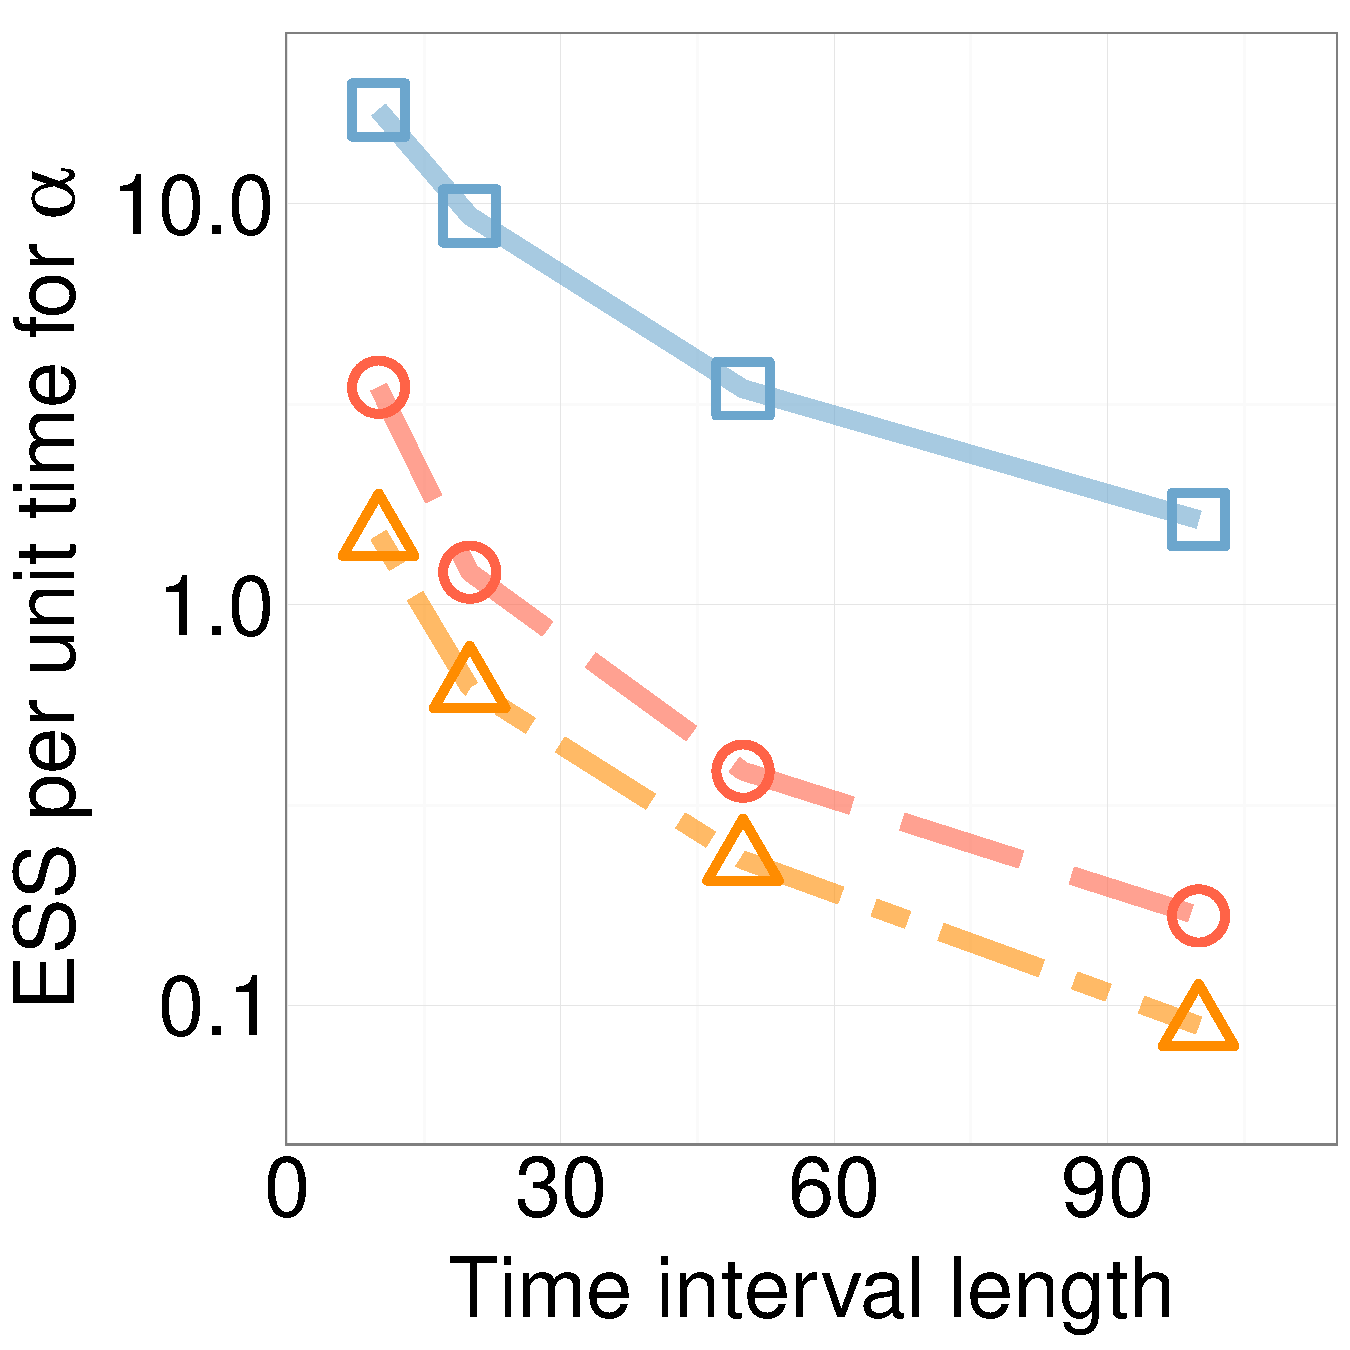
\includegraphics [width=0.40\textwidth, angle=0]{figs/ESS_vs_t_alpha_fixobservation_JC.pdf}
  \end{minipage}
%  \begin{minipage}[!hp]{0.4\linewidth}
    \caption{Time Interval vs.\ ESS/sec for JC model. In the left plot, the number of 
    observations is fixed, in the right, this grows linearly with the
  interval length. Red, yellow and blue curves are the symmetrized MH,
  \naive\ MH and Gibbs. }
	\label{fig:jc_model_vs_t}
%  \end{minipage}
%  \vspace{-.4in}
  \end{figure}
  \begin{figure}[H]
%    \vspace{-.2in}
  \centering

  \begin{minipage}[!hp]{0.99\linewidth}
  	\centering
    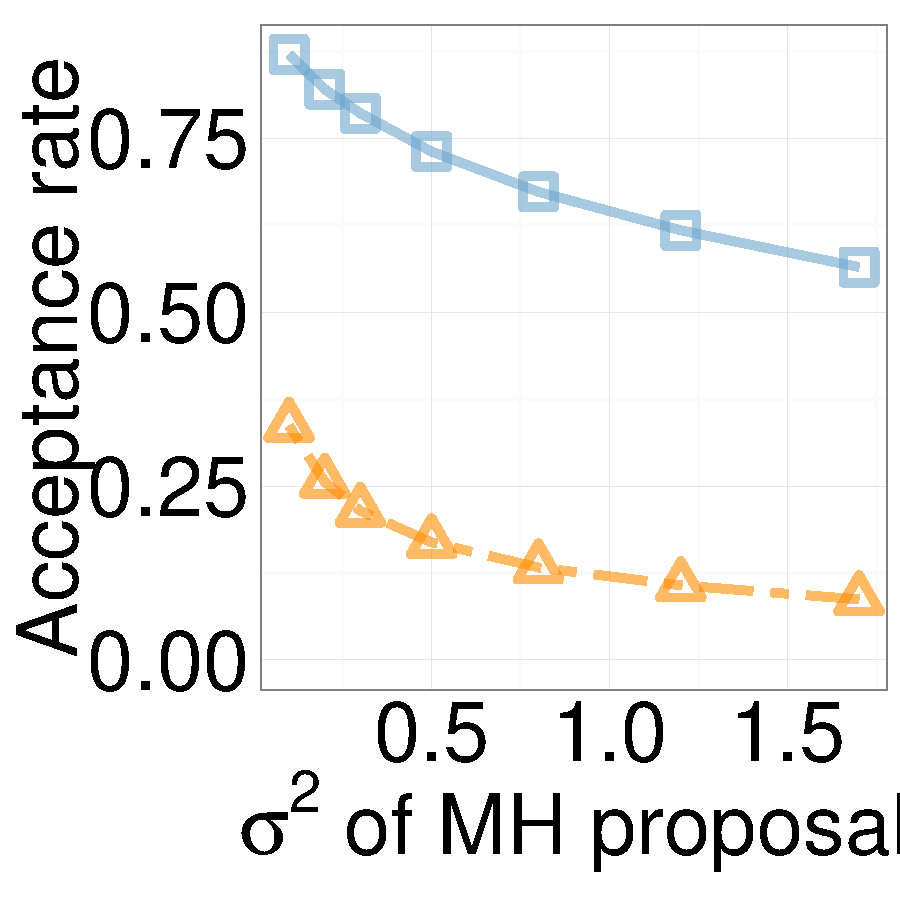
\includegraphics [width=0.40\textwidth, angle=0]{figs/acc/JCalpha_k2.pdf}
	\hspace{.5in}
    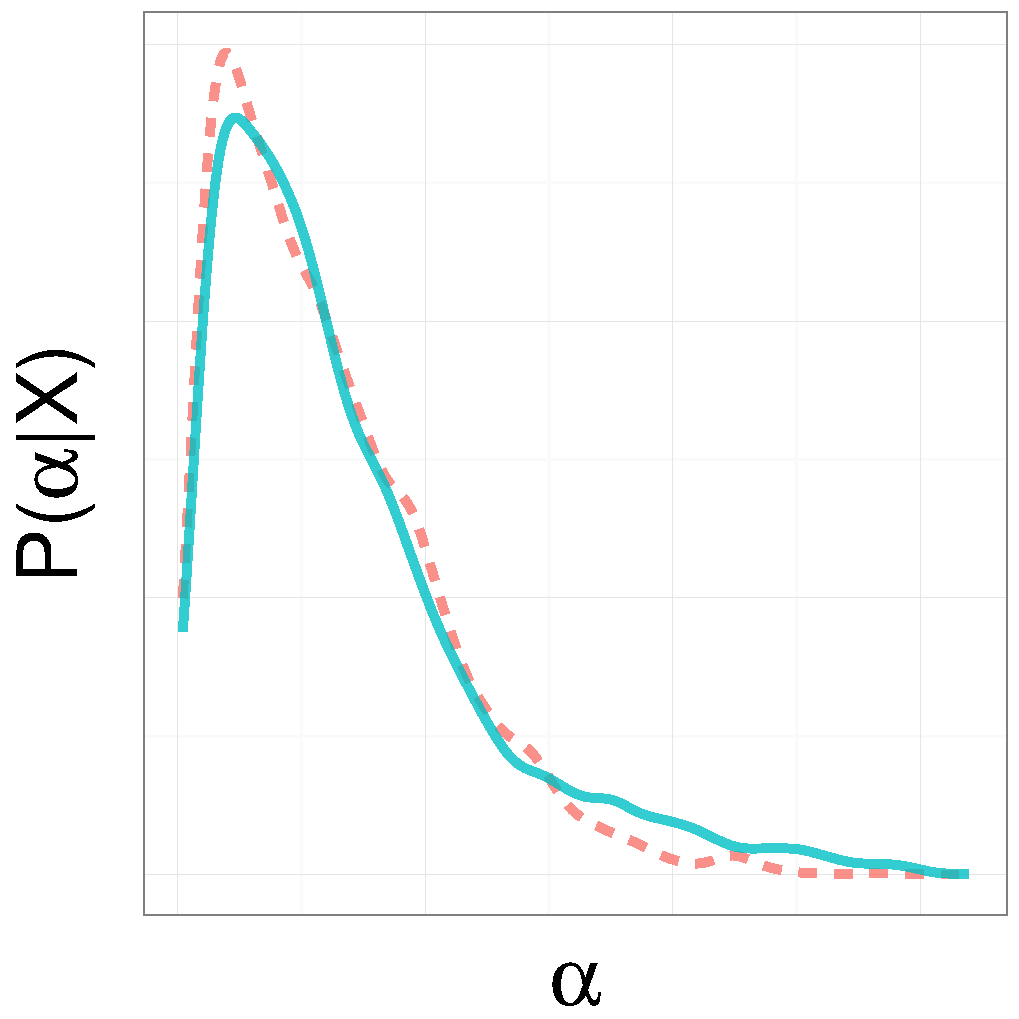
\includegraphics [width=0.40\textwidth, angle=0]{figs/JC_ks/jc_hist_44_05_3_.pdf}
  \end{minipage}
%  \begin{minipage}[!hp]{0.99\linewidth}
    \caption{The left represents the acceptance rate for $\alpha$ in the JC69 model.  Yellow and blue curves represent symmetrized MH,and \naive\ MH  algorithm. The multiplicative factor is $2$.The right is histogram for the posterior samples($\alpha$ ) of the JC69 model, the red and blue curves are the Gibbs and symmetrized MH. The p value of the two sample-Kolmogorov Smirnov test is $ 0.97$.  }
     \label{fig:ACC_JC}
%  \end{minipage}
  \end{figure}

  \begin{figure}[H]
%    \vspace{-.2in}
  \centering
%  \begin{minipage}[!hp]{0.99\linewidth}
 % \centering
  \begin{minipage}[!hp]{0.97\linewidth}
    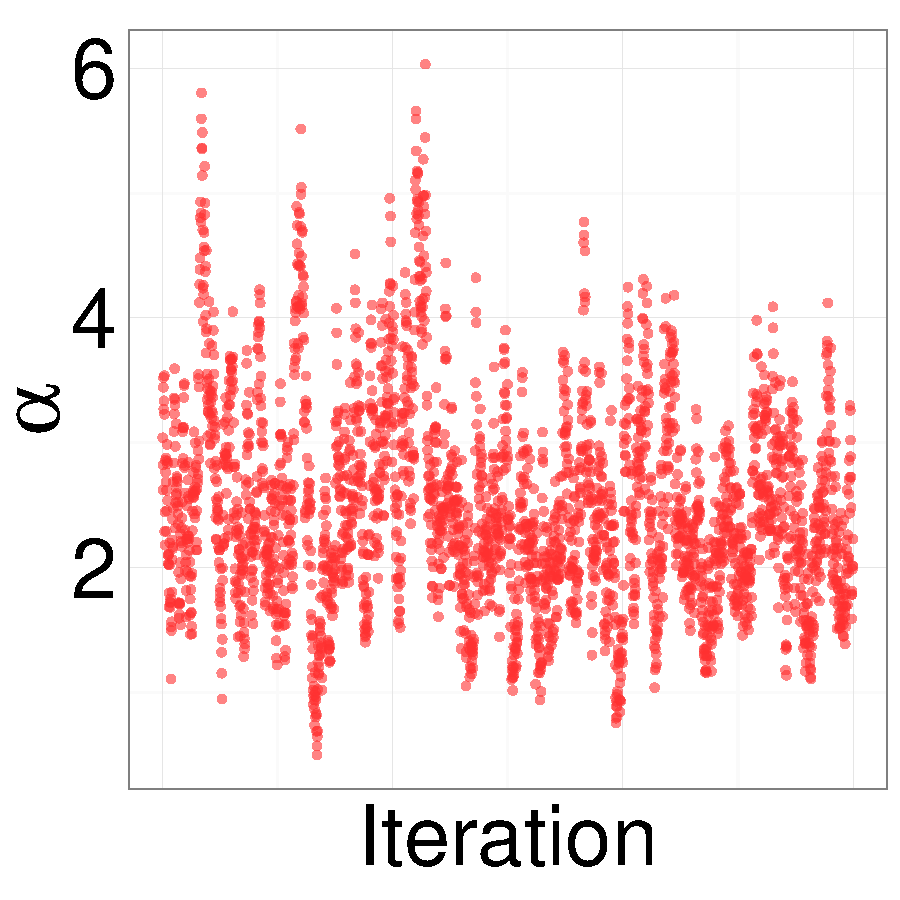
\includegraphics [width=0.40\textwidth, angle=0]{figs/JC_ks/jc_traceGBS_44_05_3_.pdf}
	\hspace{.5in}
    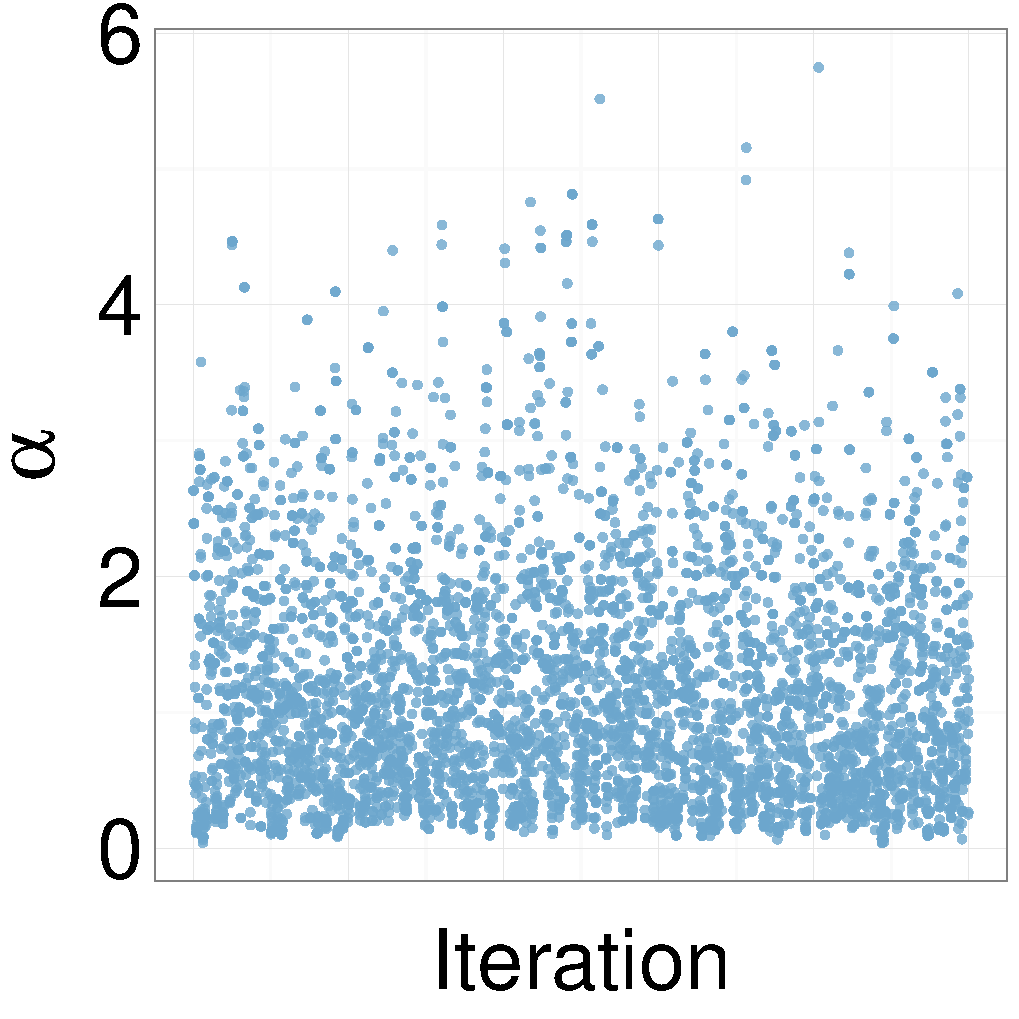
\includegraphics [width=0.40\textwidth, angle=0]{figs/JC_ks/jc_traceMH_44_05_3_.pdf}
  \end{minipage}

%  \end{minipage}
%  \begin{minipage}[!hp]{0.99\linewidth}
    \caption{Trace plots for the posterior samples of the JC69 mode, the left is for Gibbs and the right is for symmetrized MH}
     \label{fig:TRACE_JC}
%  \end{minipage}
  \end{figure}

  \begin{figure}[H]
%    \vspace{-.2in}
  \centering
  \begin{minipage}[!hp]{0.99\linewidth}
    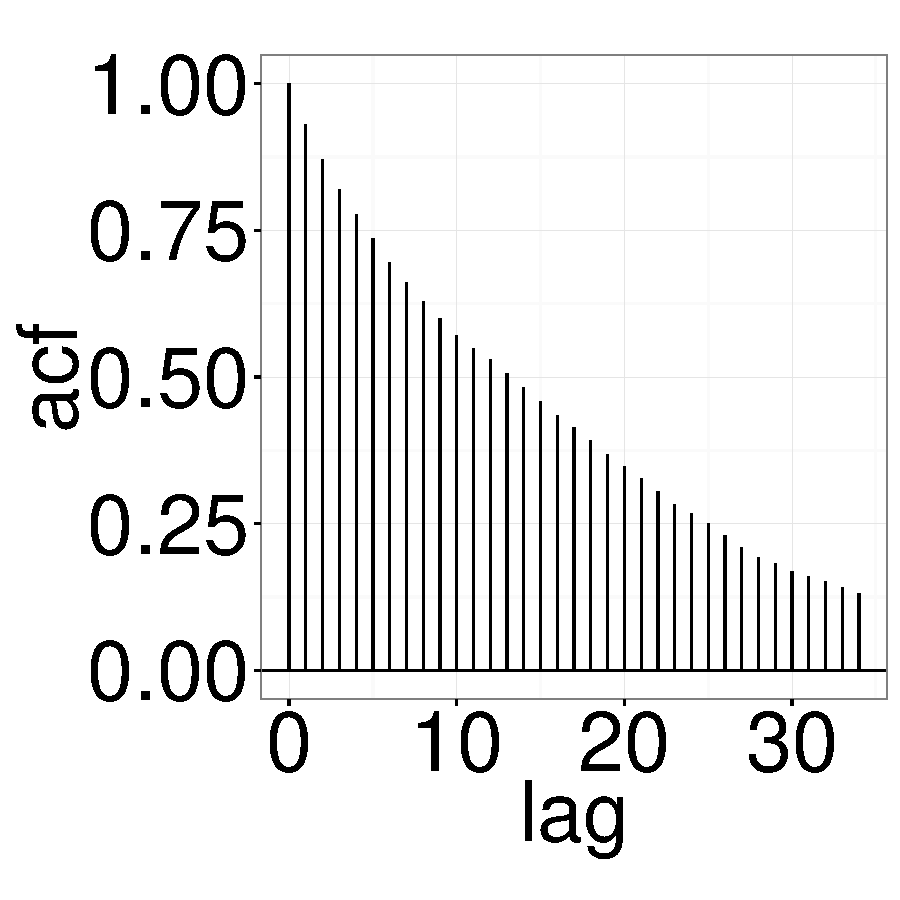
\includegraphics [width=0.40\textwidth, angle=0]{figs/JC_ks/jc_gbsacf_44_05_3_.pdf}
	\hspace{.5in}
    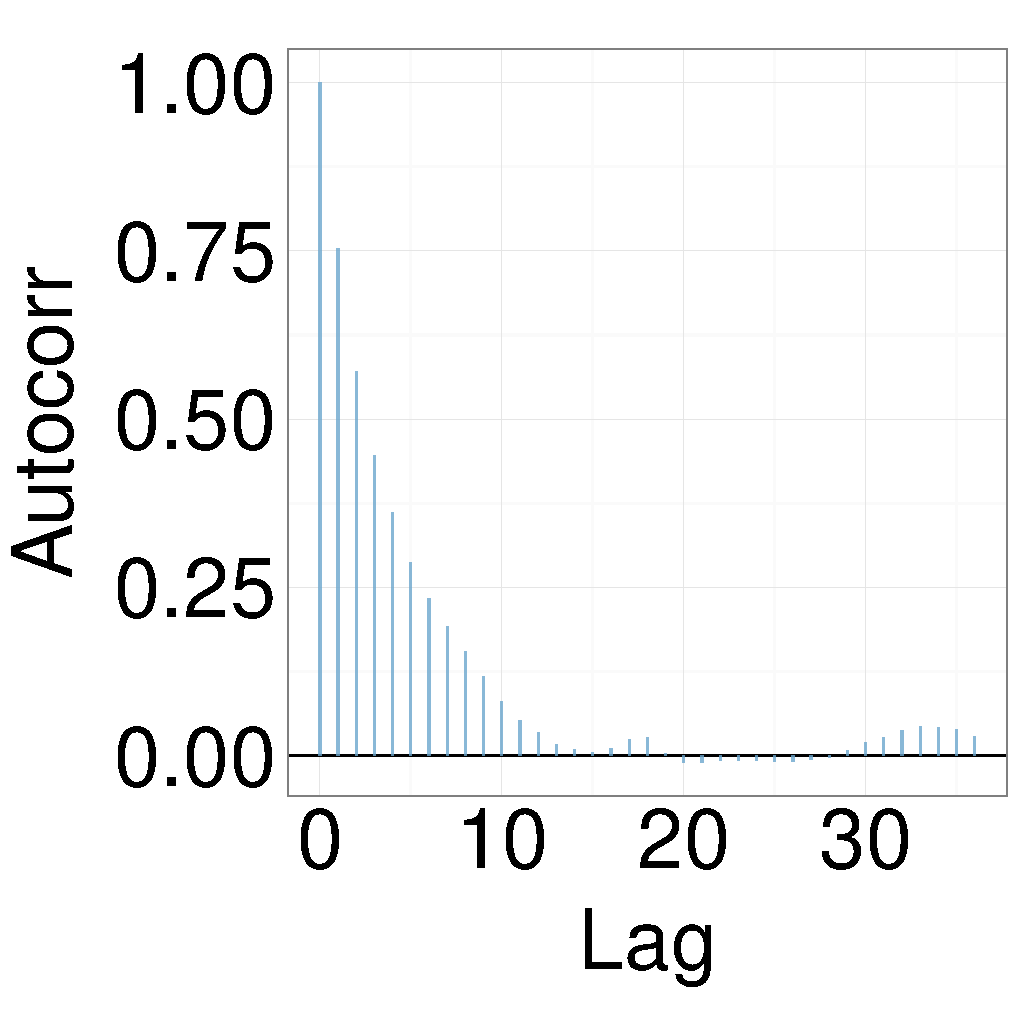
\includegraphics [width=0.40\textwidth, angle=0]{figs/JC_ks/jc_mhacf_44_05_3_.pdf}
  \end{minipage}

%  \begin{minipage}[!hp]{0.99\linewidth}
    \caption{ACFs for the posterior samples $\alpha$ of the JC69 model. The left is for Gibbs, and the right is for symmetrized MH.}
     \label{fig:ACF_JC}
%  \end{minipage}
  \end{figure}

In figure~\ref{fig:jc_model_vs_t}, we plot the ESS per unit time for the
different samplers as we increase the observation interval. In the left plot,
we keep the number of observations fixed, in the right, these increase with
the observation interval. Once again we see that our proposed algorithm
1) performs best over all interval lengths, and 2) suffers a performance
degradation with interval length that is much milder than the other algorithms.
%$$p(\alpha) = \frac{\lambda^\mu}{\Gamma(\mu)}\alpha^{\mu -1}e^{-\lambda \alpha} $$.
%Then we can get the posterior distribution $$f(\alpha | s_0,S,T)$$ as follows.
%$$ f(\alpha| s_0,S,T) \propto \exp(-(\lambda + 3(t_{end} - t_{start}))\alpha) \alpha^{\mu + N -1} .$$
%$\alpha | s_0,S,T$ is following $Gamma(\mu+ N,\lambda + 3(t_{end} - t_{start}))$\\

%  \vspace{-.25in}
\subsection{An immigration model with finite capacity}\label{sec:immig}~
Next, we consider an M/M/N/N queue~\citep{gross2011fundamentals}. The state space of this is stochastic 
process is $\{0, 1, 2, 3, \cdots, N - 1\}$ with 
elements giving the number of customers/jobs/individuals in a system/population. 
Arrivals follow a rate-$\alpha$ Poisson process, moving the process from state 
$i$ to $i+1$ for $i<N$. The system has a capacity of $N$, so any arrivals when 
the current state is $N$ are discarded.  Service times or deaths are 
exponentially distributed, with a rate that is now state-dependent:
the system moves from $i$ to $i - 1$ with rate $i\beta$. 
%There are $N$ servers, which serve from the front of the queue. 
%If there are less than $N$ jobs, some of the servers will be idle. 
%Only $N$ customers can queue at any one time. 
%Any further arrivals to the queue are considered ''lost''. 

% \begin{figure}
% \centering
% \begin{minipage}[hp]{0.6\linewidth}%0.45
% \centering
%   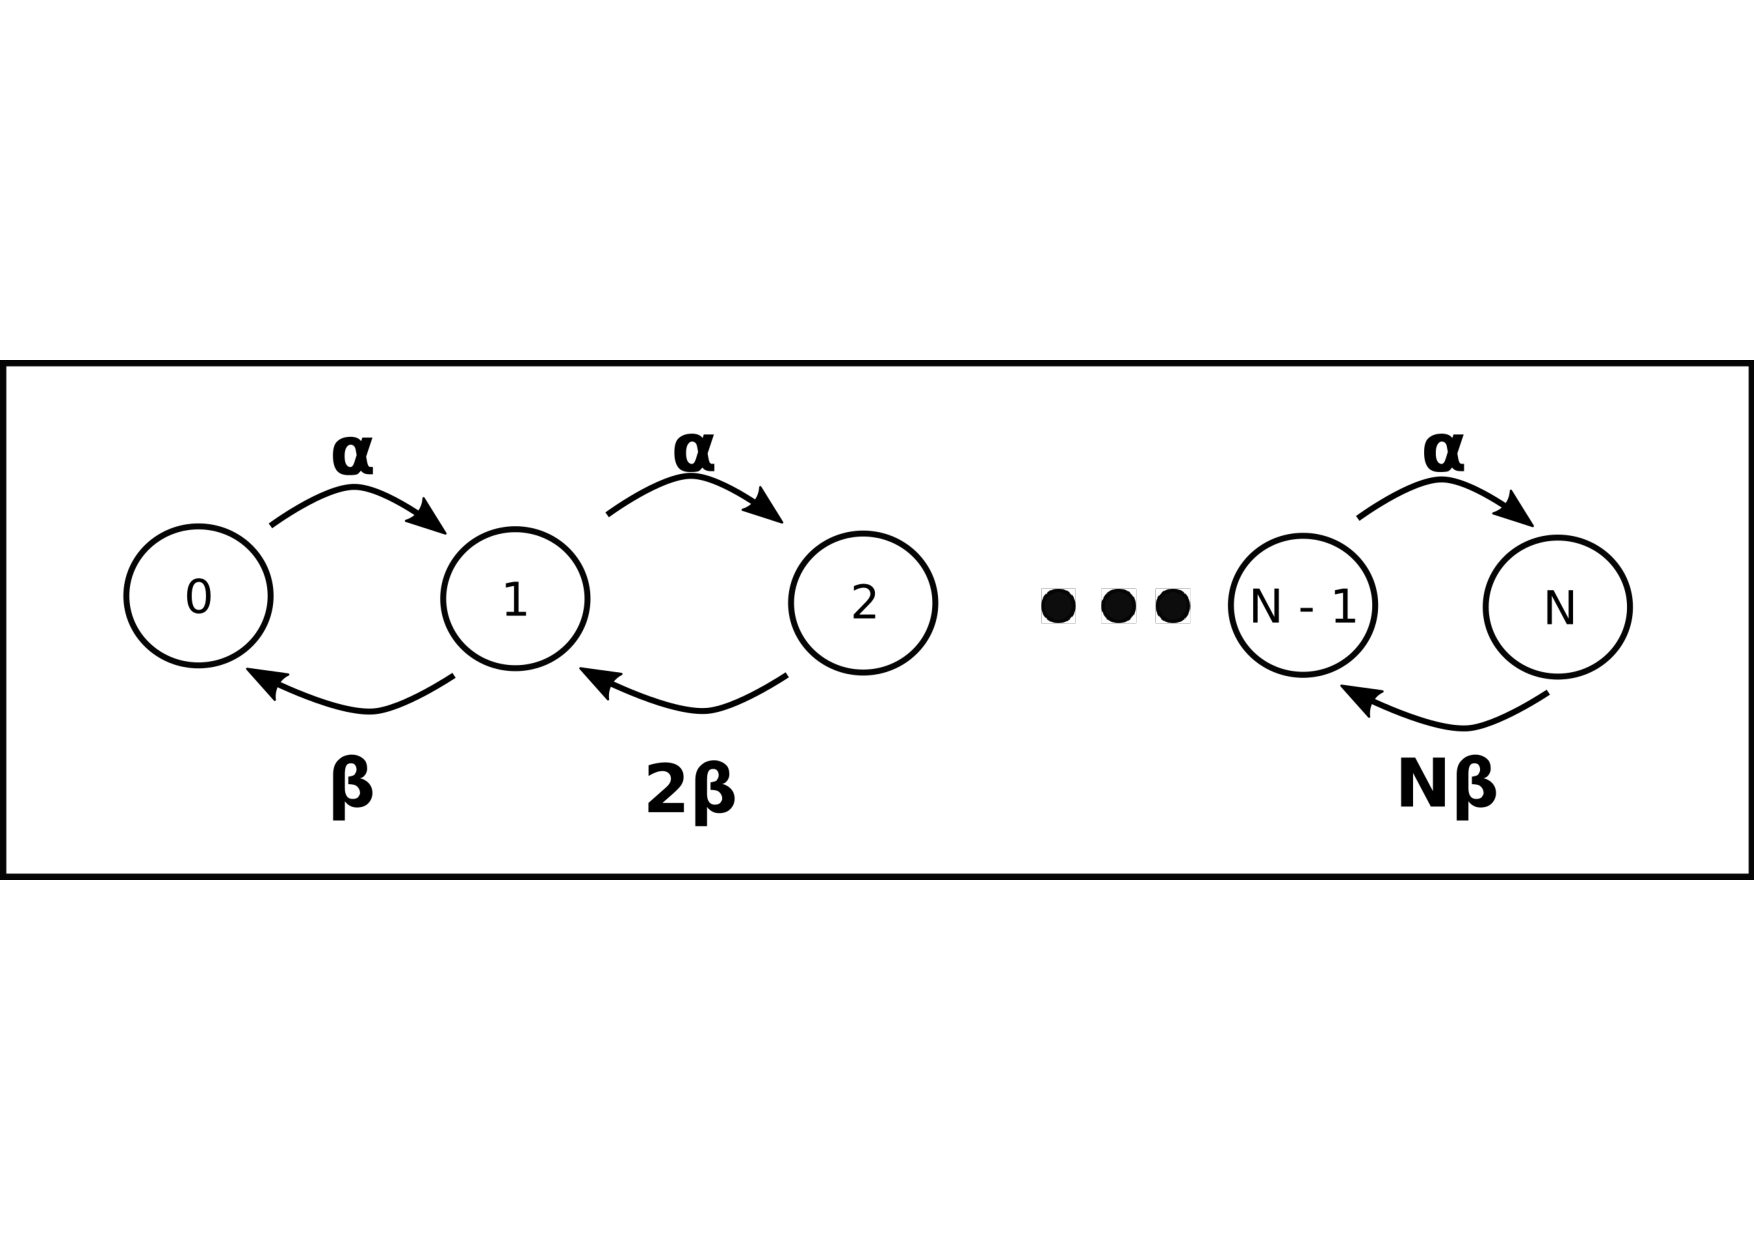
\includegraphics [width=1\textwidth, angle=0]{figs/queue_model.pdf}%0.70
%     \end{minipage}
%   \caption{queuing model}
%   \label{q_model}
% \end{figure}
  \begin{figure}%[b]
  \centering
  \begin{minipage}[hp]{0.99\linewidth}
%  \begin{minipage}[hp]{0.65\linewidth}
  \centering
    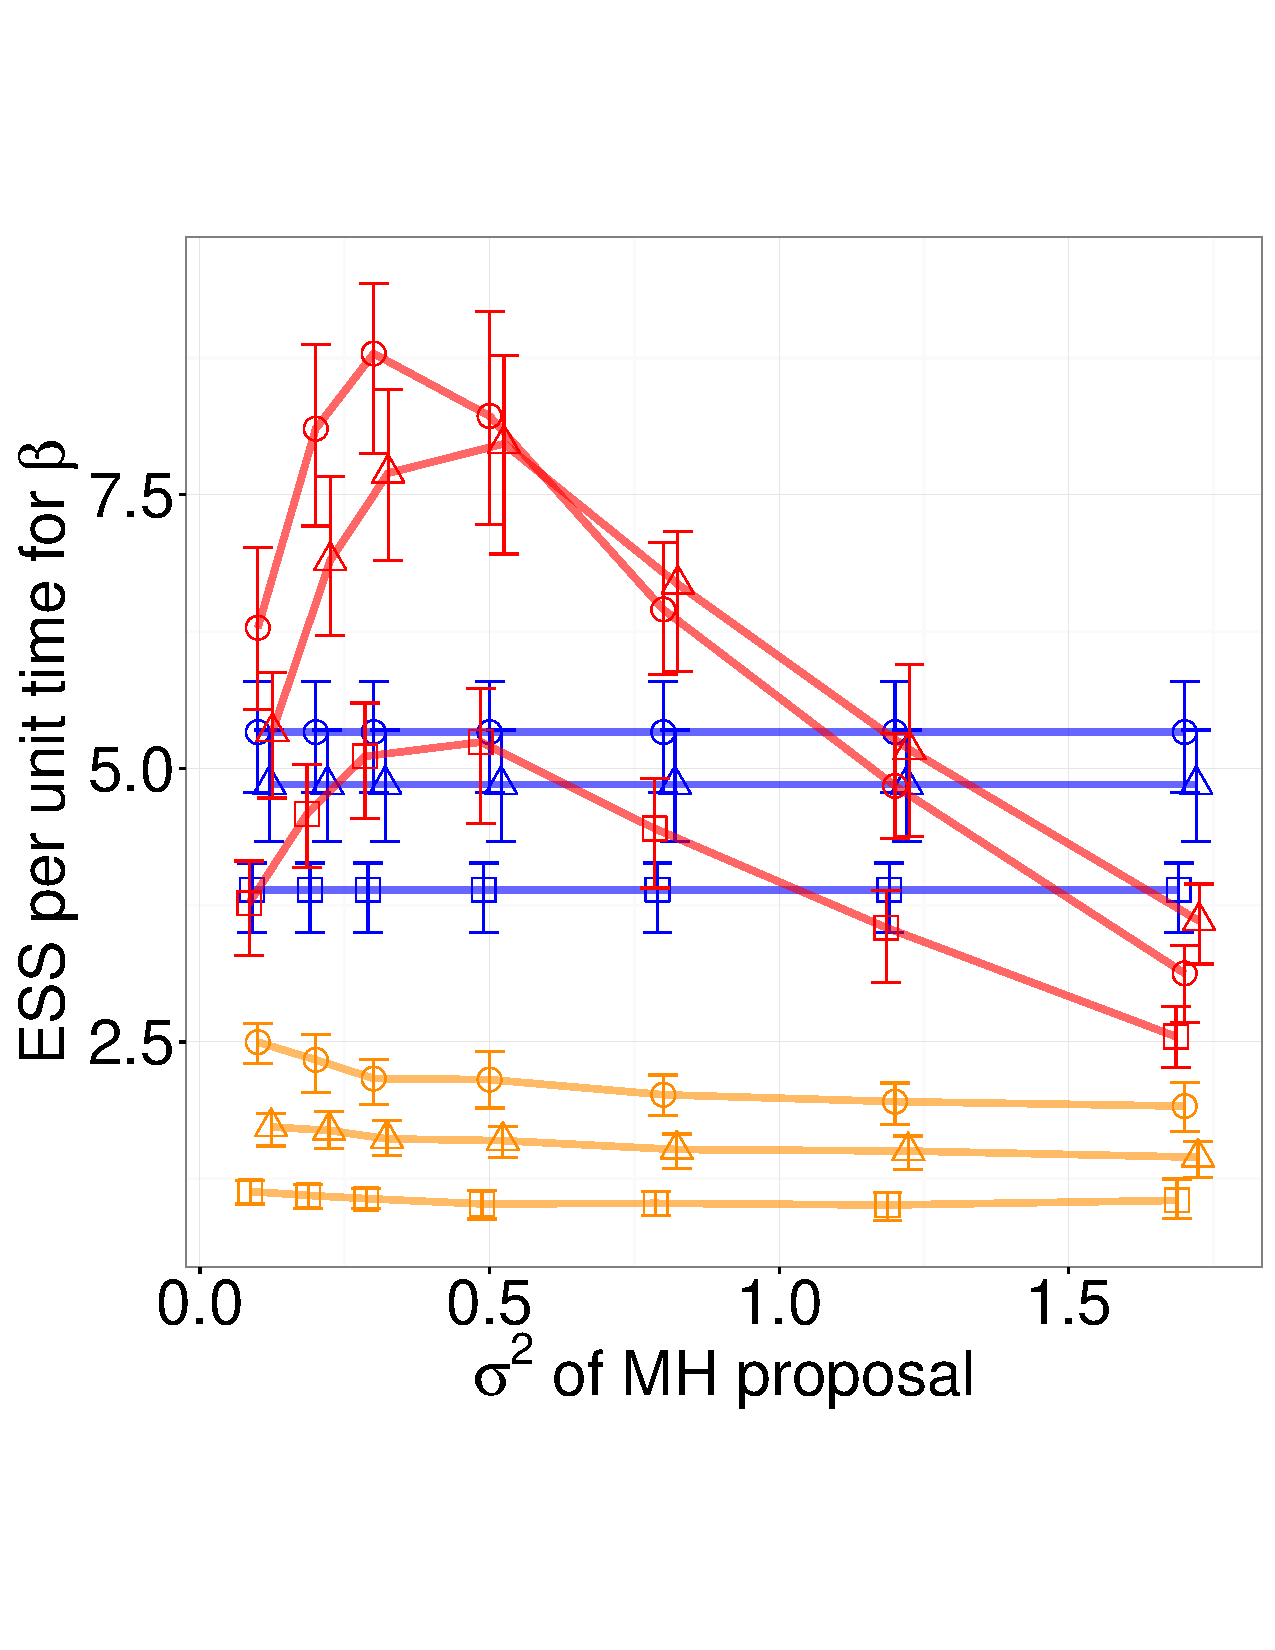
\includegraphics [width=0.41\textwidth, angle=0]{figs/q_3_alpha.pdf}
    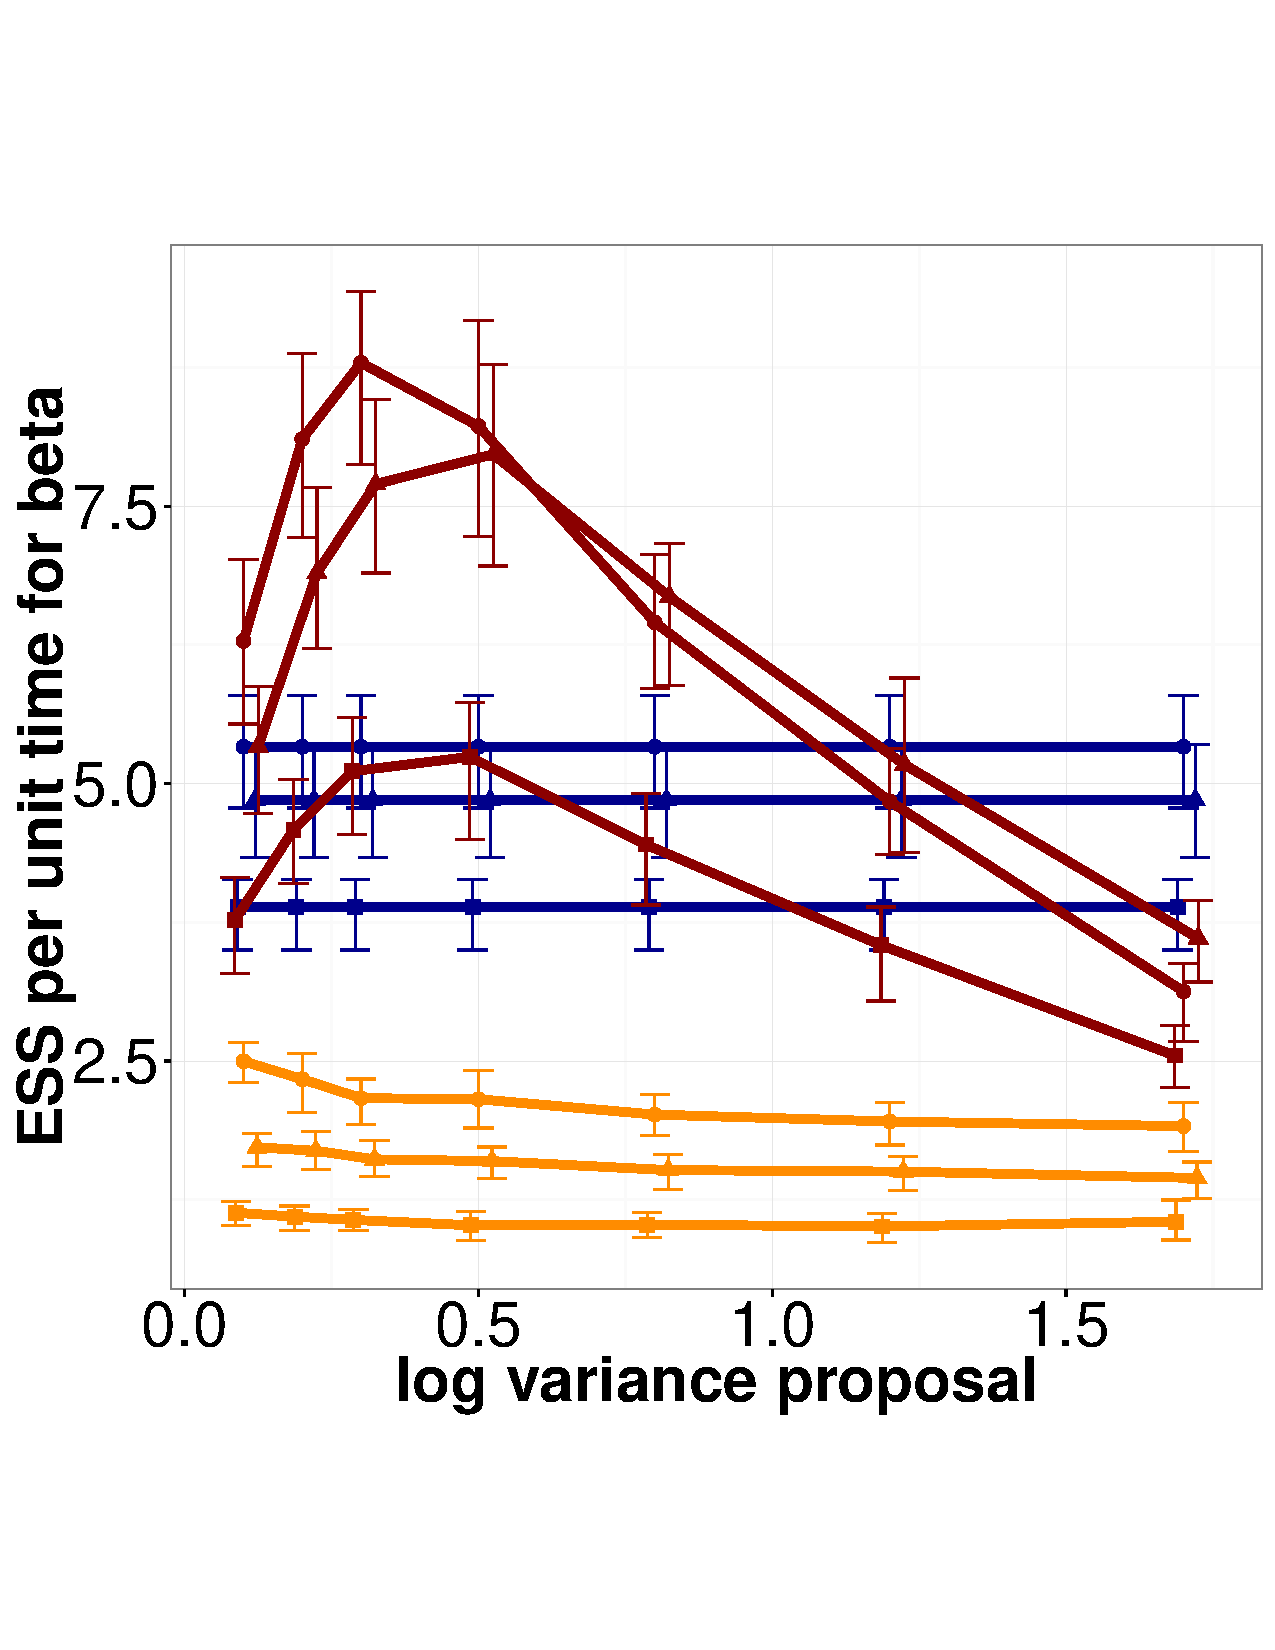
\includegraphics [width=0.41\textwidth, angle=0]{figs/q_3_beta.pdf}
    \vspace{-.1 in}
  \centering
    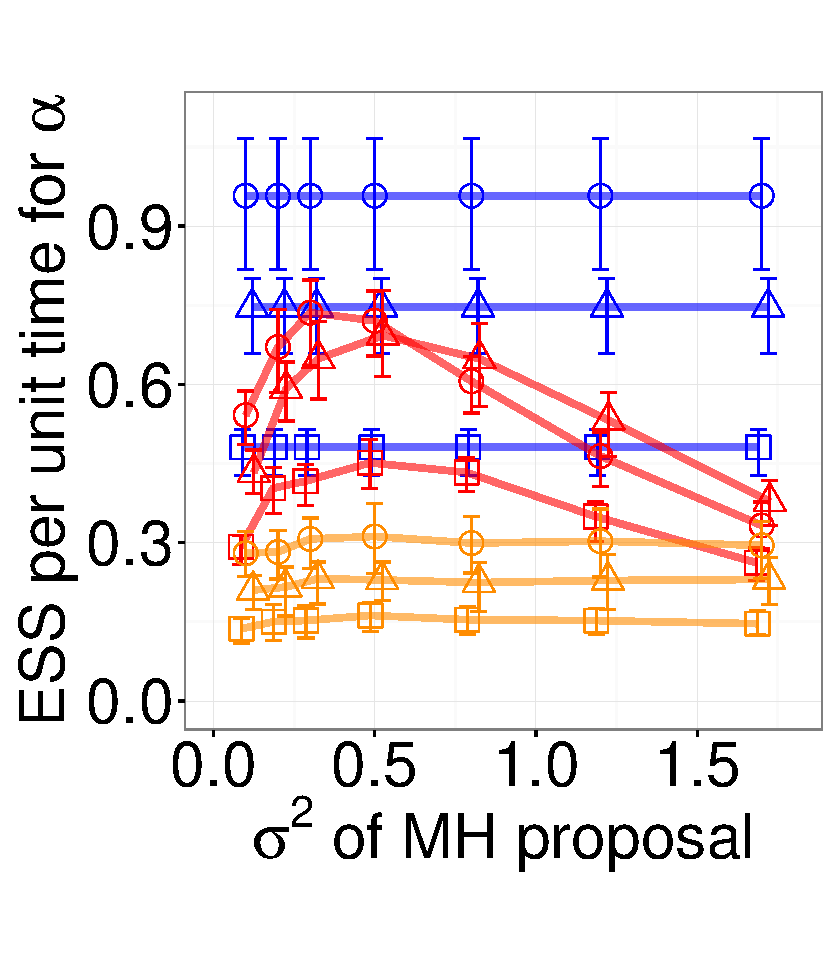
\includegraphics [width=0.41\textwidth, angle=0]{figs/q_10_alpha.pdf}
    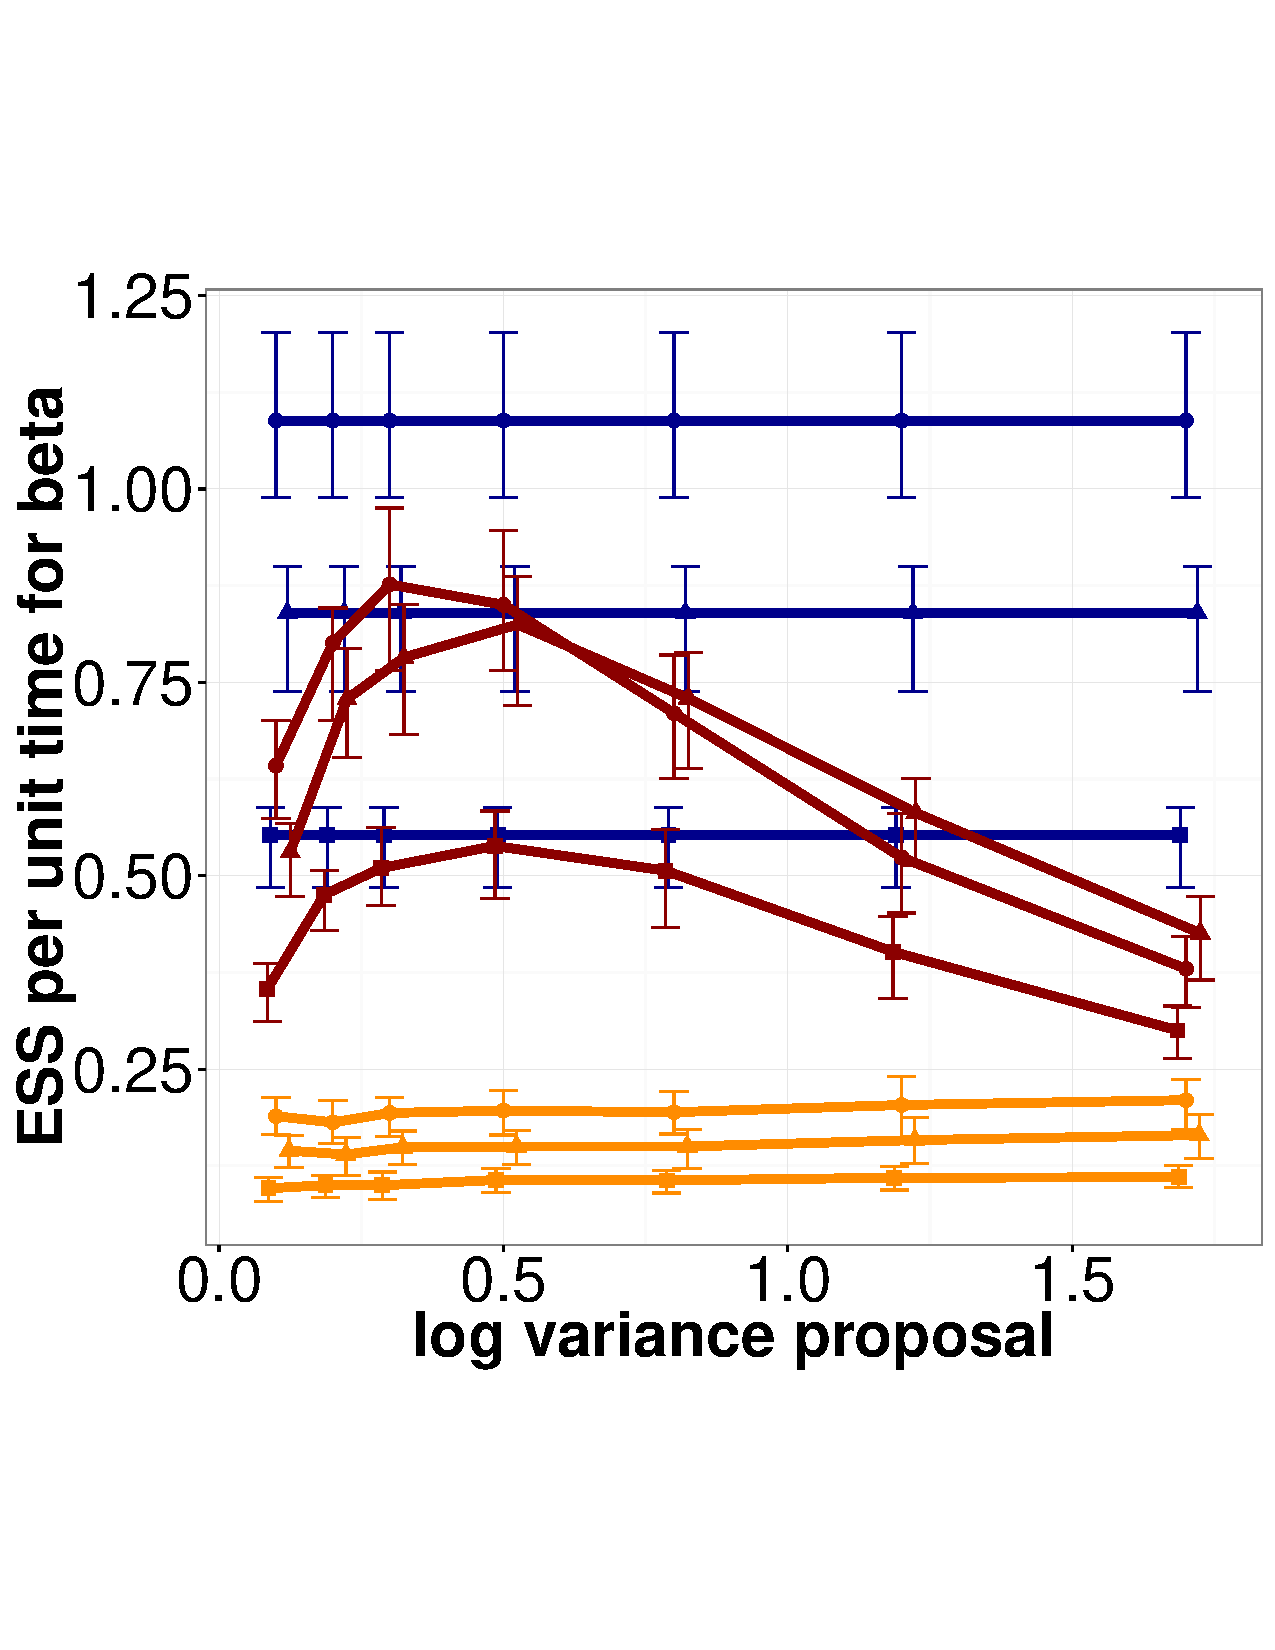
\includegraphics [width=0.41\textwidth, angle=0]{figs/q_10_beta.pdf}
    \vspace{-0.1 in}
  \end{minipage}
%  \begin{minipage}[!hp]{0.33\linewidth}
    \caption{ESS/sec for the immigration model, the top row being dimension 3, and the bottom,
      dimension 10. The left column is for $\alpha$, and the 
    right is for $\beta$. Red, yellow, and blue curves are the symmetrized MH,
  \naive\ MH, Gibbs sampling and particle MCMC.}
     \label{fig:ESS_Q_D10}
%  \end{minipage}
%  \vspace{-.4in}
  \end{figure}
  \begin{figure}[H]
%    \vspace{-.2in}
  \centering

  \begin{minipage}[!hp]{0.99\linewidth}
    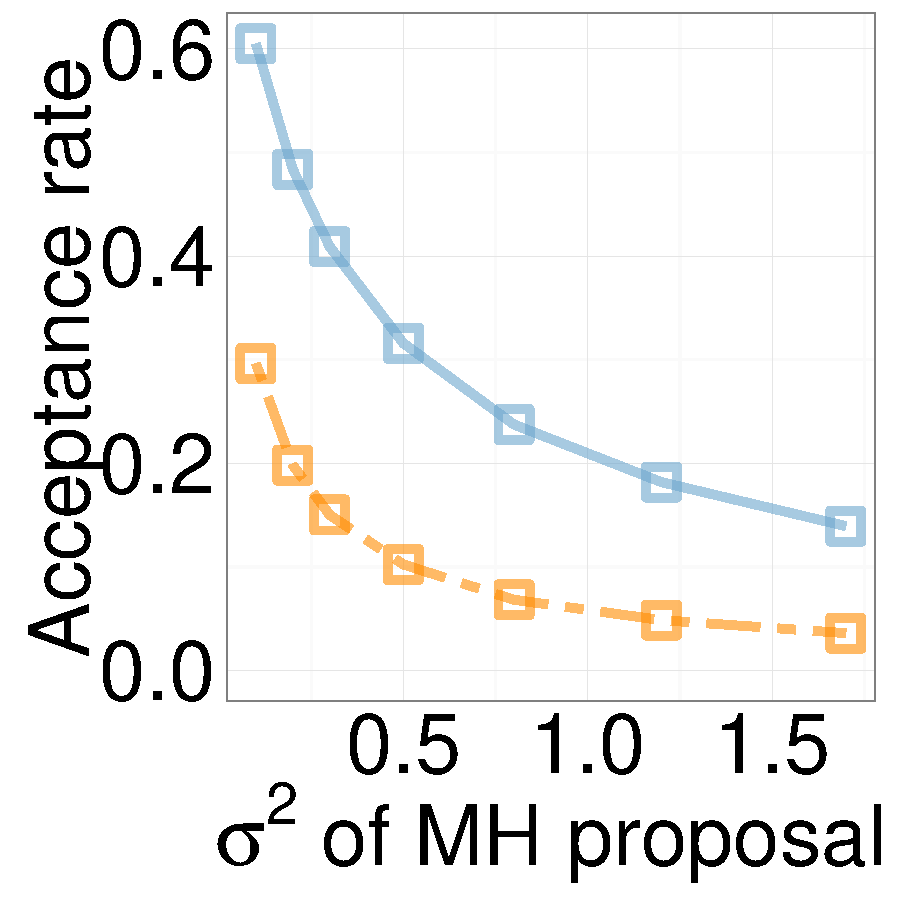
\includegraphics [width=0.40\textwidth, angle=0]{figs/acc/Q_D3alpha_k2.pdf}
	\hspace{.5in}
    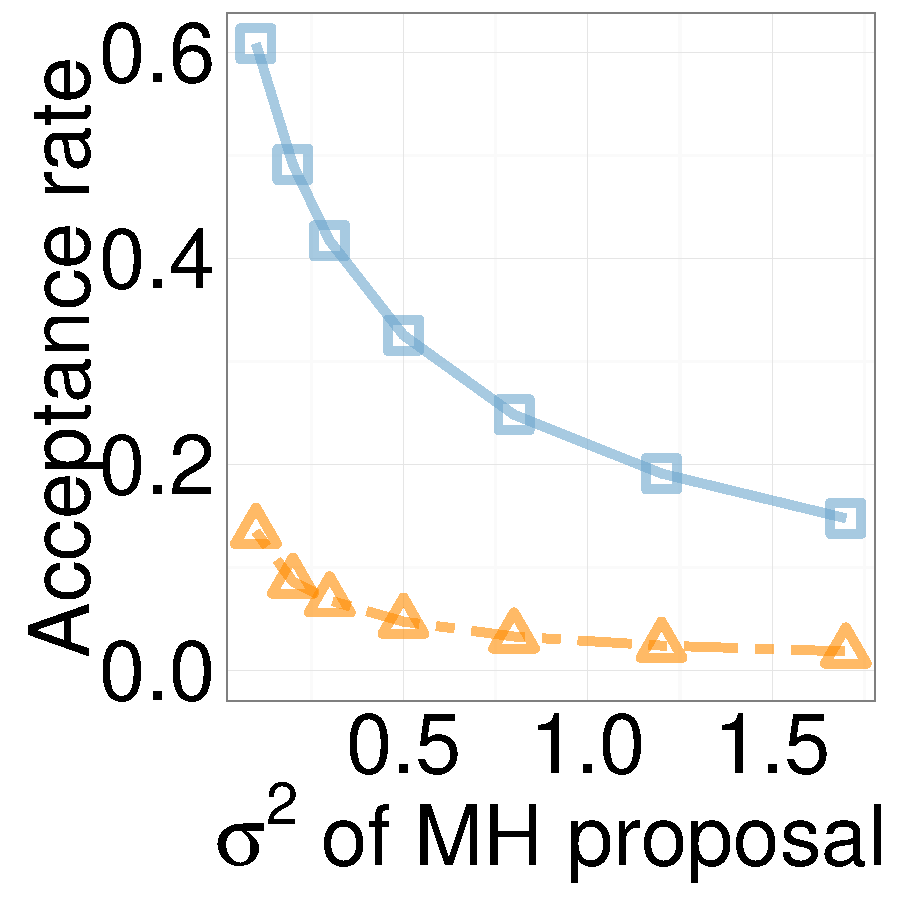
\includegraphics [width=0.40\textwidth, angle=0]{figs/acc/Q_D10alpha_k2.pdf}
  \end{minipage}
%  \begin{minipage}[!hp]{0.99\linewidth}
    \caption{Acceptance Rate for $\alpha$ in the synthetic model, the left row being dimension 3, and the right,dimension 10.  Yellow and blue curves represent symmetrized MH,
 and \naive\ MH  algorithm. The multiplicative factor is $2$. }
     \label{fig:ACC_Q}
%  \end{minipage}
  \end{figure}

  \begin{figure}[H]
%    \vspace{-.2in}
  \centering
%  \begin{minipage}[!hp]{0.99\linewidth}
 % \centering
  \begin{minipage}[!hp]{0.97\linewidth}
    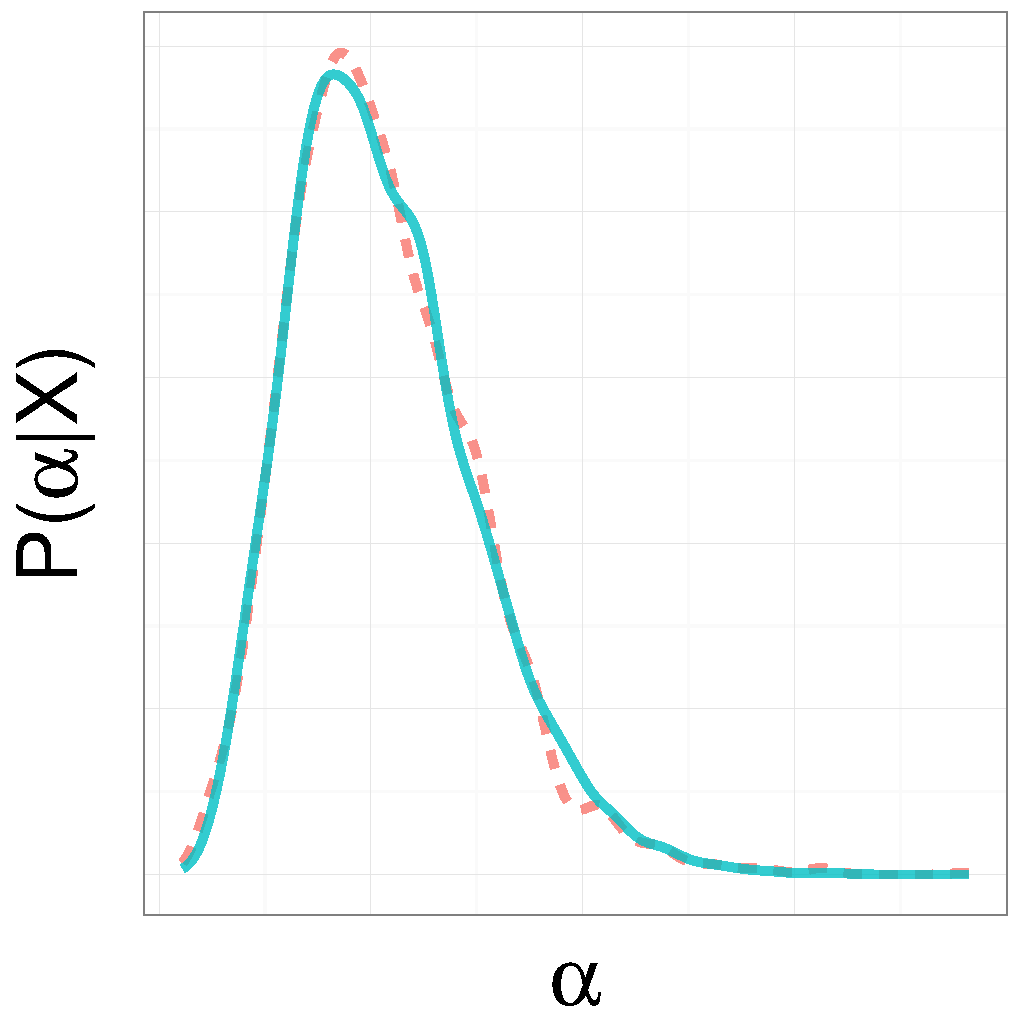
\includegraphics [width=0.30\textwidth, angle=0]{figs/Q_ks/q_hist_20_03_3_.pdf}
    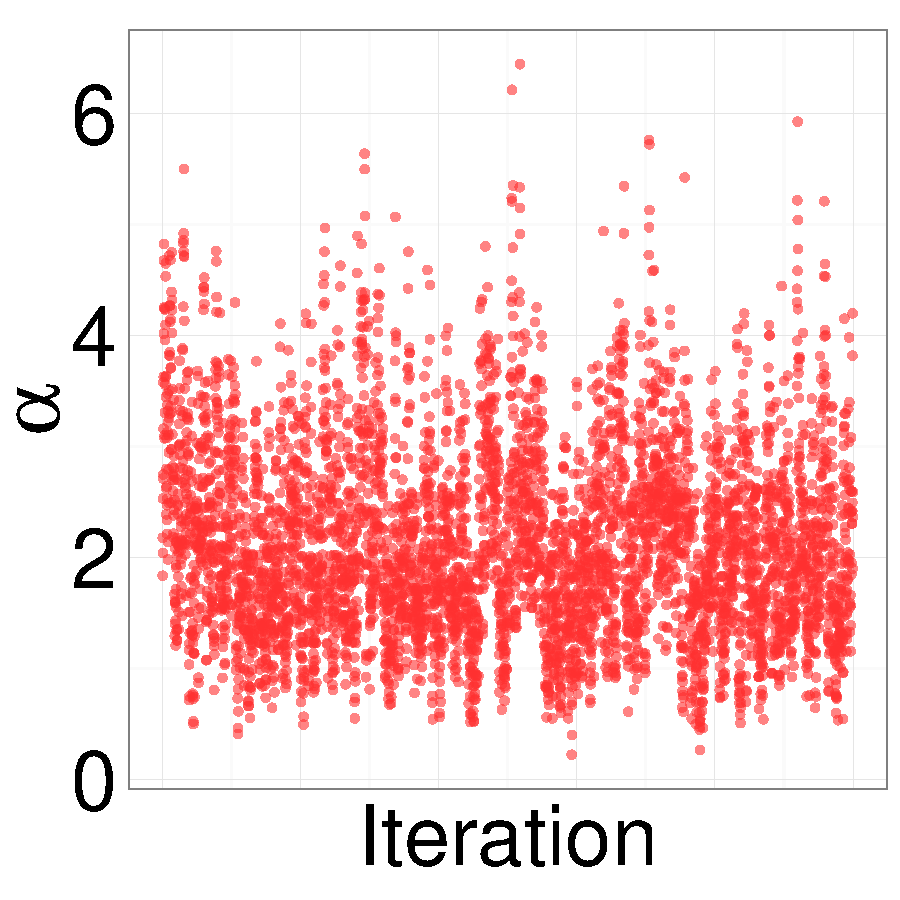
\includegraphics [width=0.30\textwidth, angle=0]{figs/Q_ks/q_traceGBS_20_03_3_.pdf}
    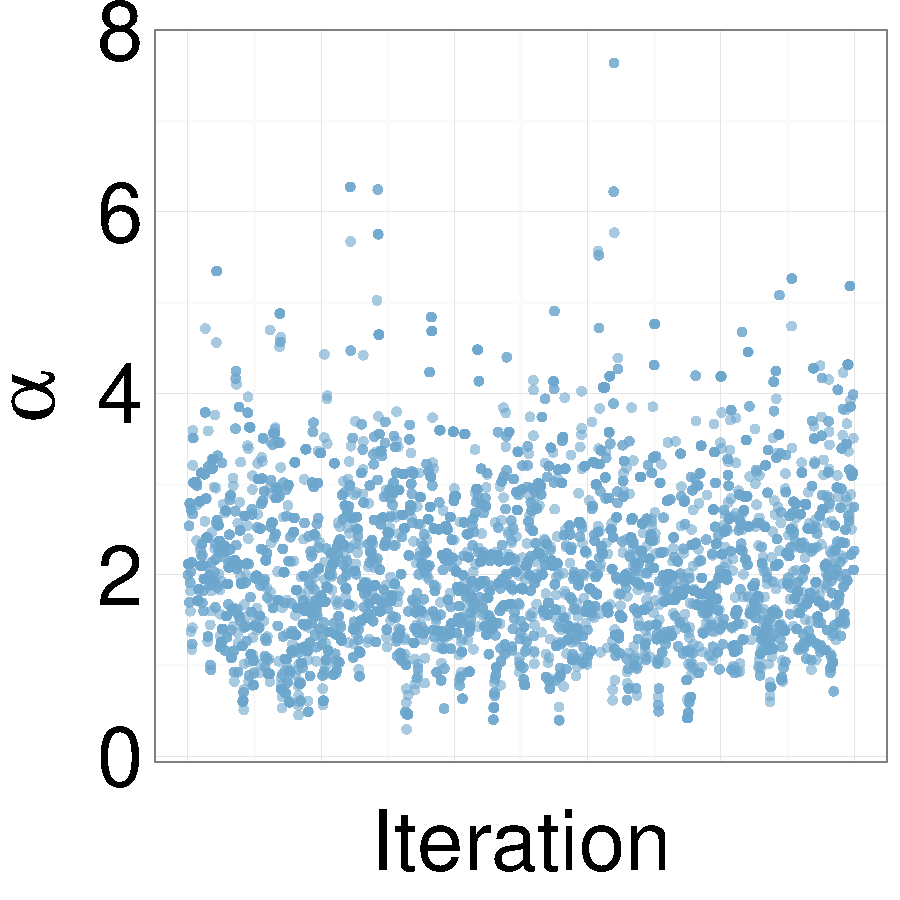
\includegraphics [width=0.30\textwidth, angle=0]{figs/Q_ks/q_traceMH_20_03_3_.pdf}
  \end{minipage}

%  \end{minipage}
%  \begin{minipage}[!hp]{0.99\linewidth}
    \caption{The left is histogram for the posterior samples($\alpha$) of the immigration model with dimension 3, the red and blue curves are the Gibbs and symmetrized MH. The p value of the two sample-Kolmogorov Smirnov test is $ 0.978$. The middle and the right are trace plots for the posterior samples of the immigration model with dimension 3, the middle is for Gibbs and the right is for symmetrized MH}
     \label{fig:TRACE_Q}
%  \end{minipage}
  \end{figure}

  \begin{figure}[H]
%    \vspace{-.2in}
  \centering
  \begin{minipage}[!hp]{0.99\linewidth}
    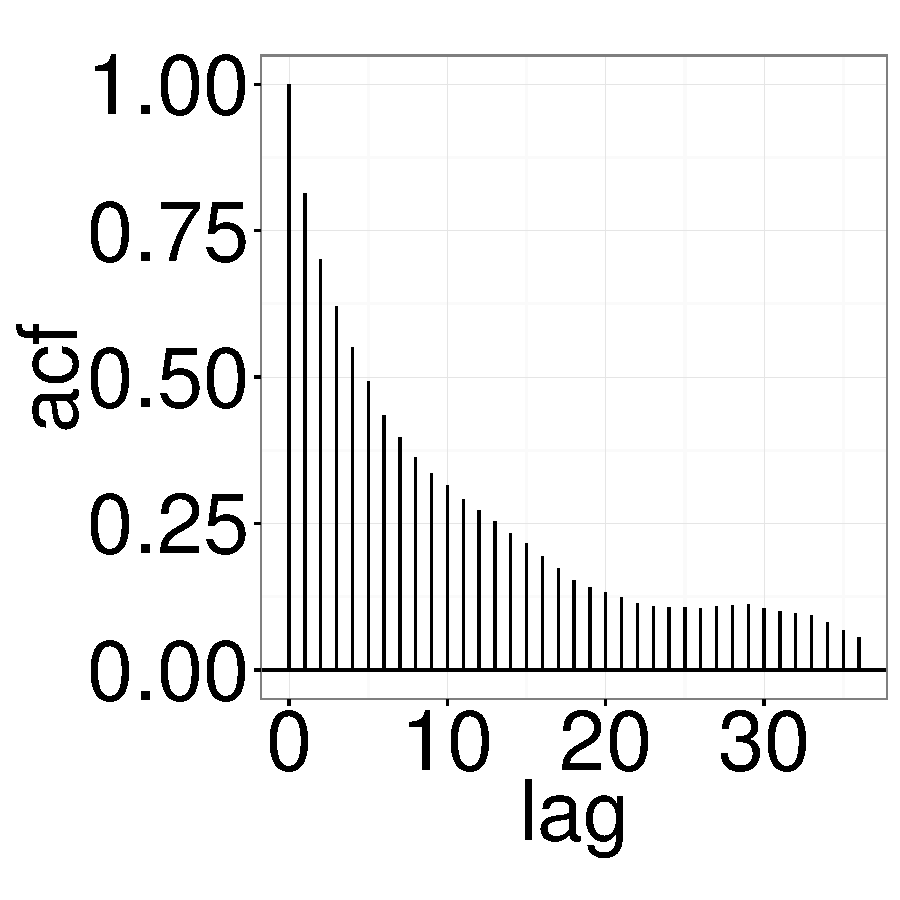
\includegraphics [width=0.40\textwidth, angle=0]{figs/Q_ks/q_gbsacf_20_03_3_.pdf}
	\hspace{.5in}
    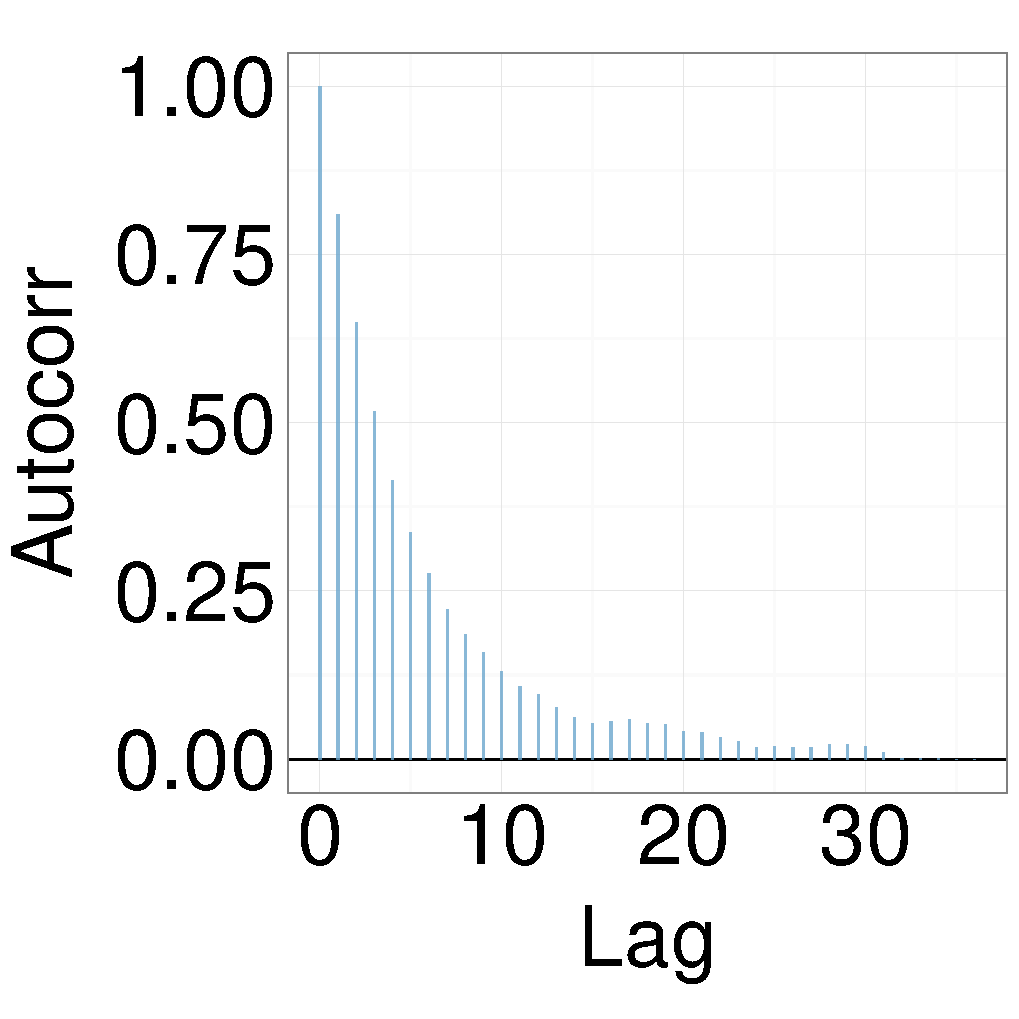
\includegraphics [width=0.40\textwidth, angle=0]{figs/Q_ks/q_mhacf_20_03_3_.pdf}
  \end{minipage}

%  \begin{minipage}[!hp]{0.99\linewidth}
    \caption{ACFs for the posterior samples $\alpha$ of the immigration model with dimension 3. The left is for Gibbs, and the right is for symmetrized MH.}
     \label{fig:ACF_Q}
%  \end{minipage}
  \end{figure}


We follow the same setup as the first experiment:
for $(\alpha_0,\alpha_1,\beta_0,\beta_1)$ equal to $(3,2,5,2)$,
we place Gamma$(\alpha_0,\alpha_1)$, and Gamma$(\beta_0, \beta_1)$ priors on 
$\alpha$, $\beta$. These prior distributions are used to sample transition 
matrices $A$, which, along with a uniform distribution over initial states,
are used to generate MJP trajectories. We observe these at integer-valued
times according to a Gaussian observation process.
We consider three settings: $3, 5$ and $10$ states, with results from $5$ 
steps included in the appendix. 

  %\subsection{Experiments}
  Figure~\ref{fig:ESS_Q_D10} plots the ESS 
  per unit time for the parameters $\alpha$ (left) and $\beta$ (right) as we 
  change the variance of the proposal kernel, for different settings of
  different algorithms. The top row shows results for a state-space
  of dimension $3$, and the bottom row, results for a dimension
  $10$.
  %Colors and types are the same as the previous experiment.
  Again, our symmetrized  MH algorithm does best for dimensions
  $3$ and $5$, although now Gibbs sampling performs well for dimensionality $10$.
  This is partly because for this problem, the Gibbs conditionals over $\alpha$
  and $\beta$ are conjugate, and have a very simple Gamma distribution
  (this is also why the Gibbs sampler curves are straight lines: there is no
  proposal distribution involved here).
% Figure~\ref{fig:hist} shows posterior distributions for 
% $P(\theta | X)$(red), $P(\theta | S, T, X)$(green), $P(\theta | W, X)$(blue). 
% We run $10000$ iterations. The first $5000$ are treated as burn in period. 
% We fix $V_{5000}, W_{5000}$ and then sample $\theta$ from 
% $P(\theta | V_{5000}, W_{5000}, X)$ and sample $\theta$ from 
% $P(\theta | W_{5000}, X)$. We keep updating $S$ and $T$ for sampling from 
% $P(\theta | X)$. We sample another $5000$ $\theta$s to draw the histograms. 
% We can find that $P(\theta | S, T, X)$ and $P(\theta | W, X)$ are both very 
% concentrated which implies the coupling.
% \begin{figure}%[b]
% \begin{minipage}[hp]{0.45\linewidth}
% \centering
%   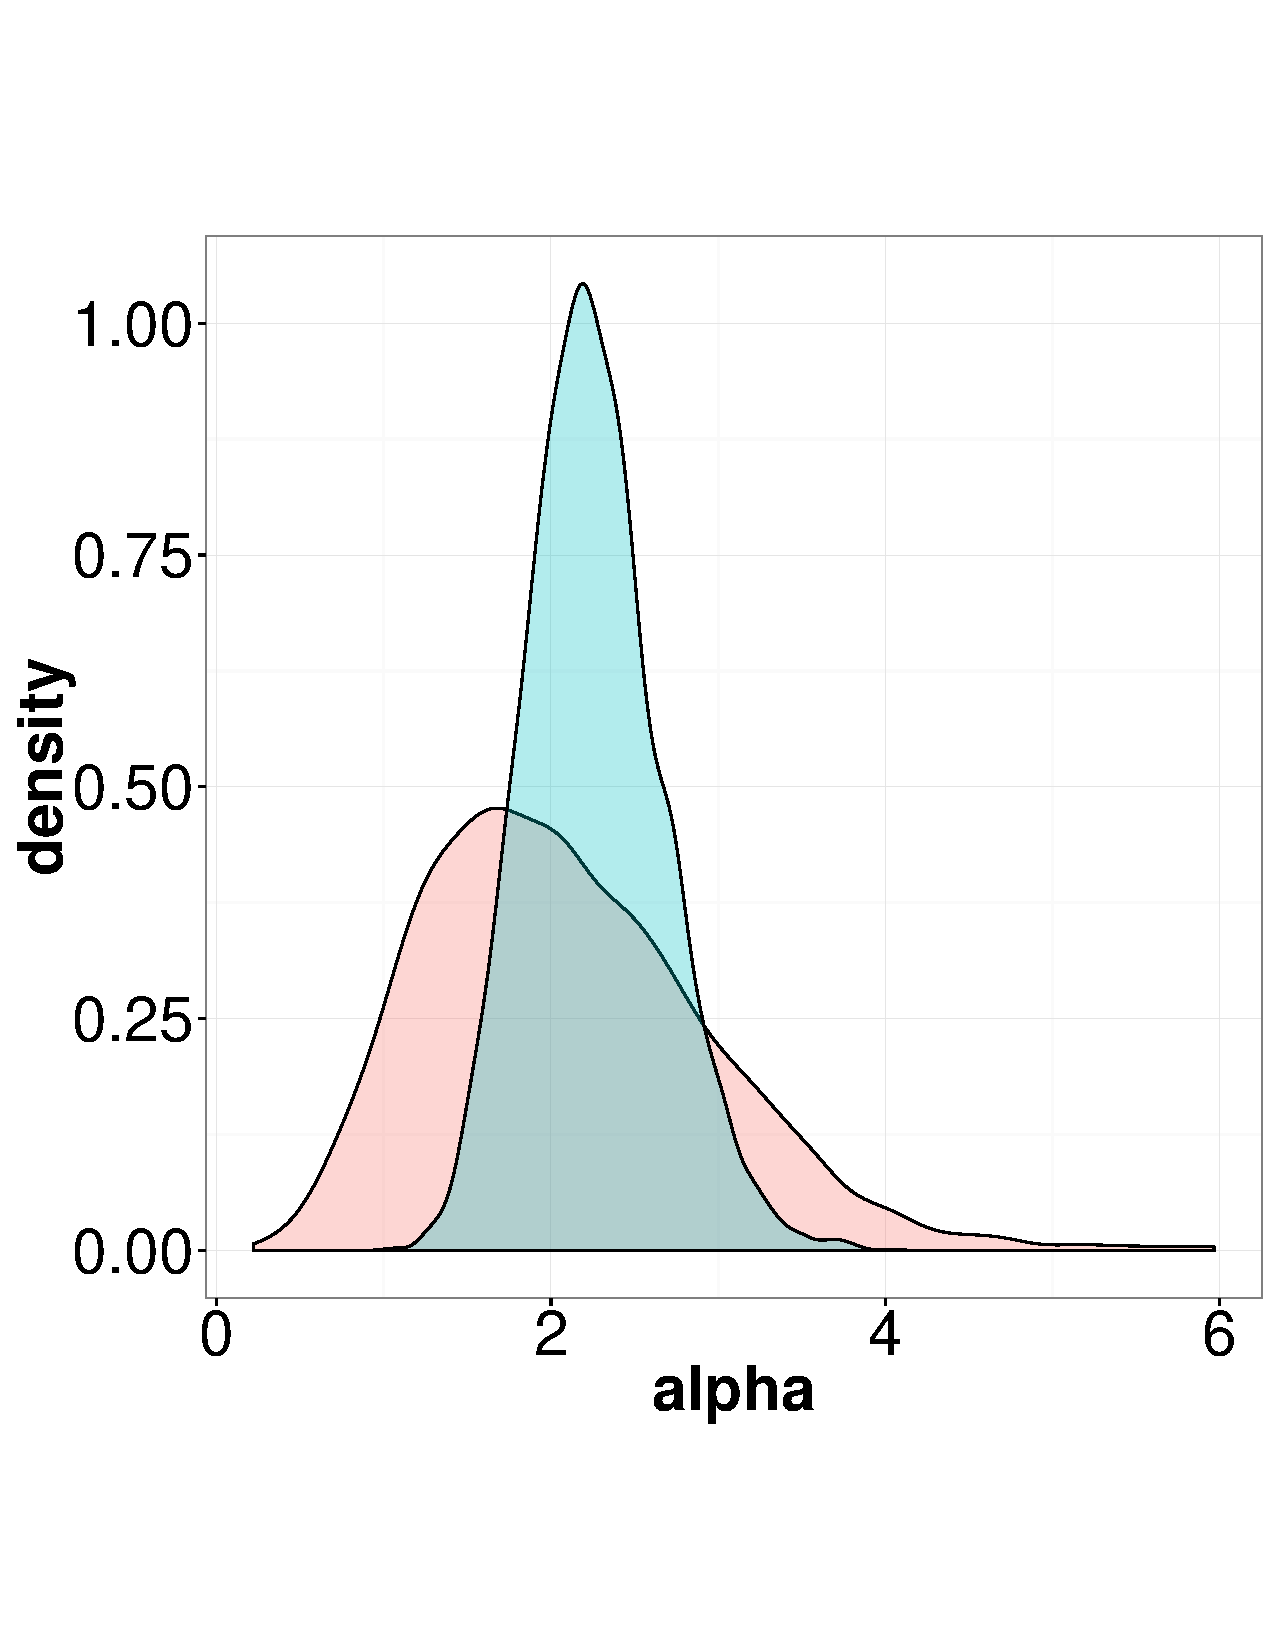
\includegraphics [width=0.90\textwidth, angle=0]{figs/dist_alpha.pdf}
%   \vspace{-0 in}
% \end{minipage}
% \begin{minipage}[!hp]{0.45\linewidth}
% \centering
%   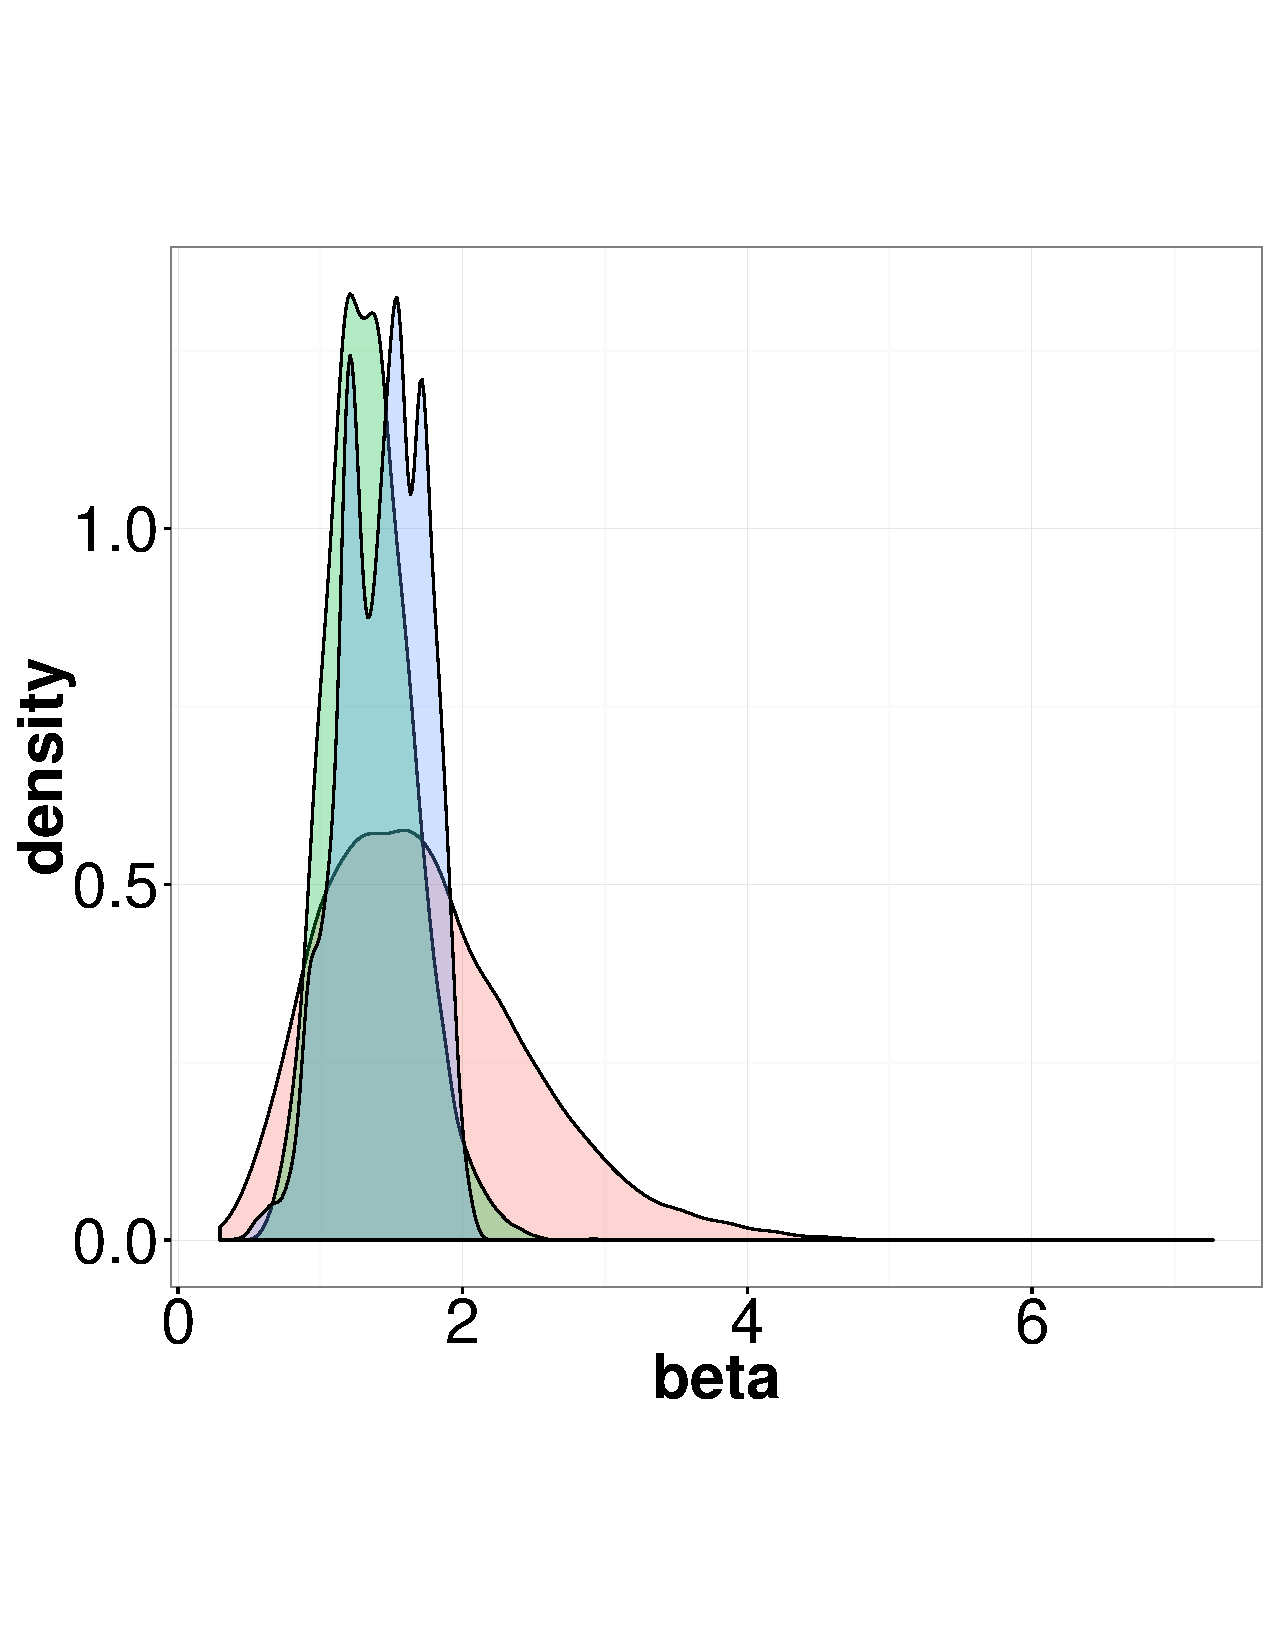
\includegraphics [width=0.90\textwidth, angle=0]{figs/dist_beta.pdf}
%   \vspace{-0 in}
% \end{minipage}
%   \caption{density.The left is for $\alpha$, and the right is for $\beta$.}
%    \label{fig:dist}
% \end{figure}
% $w(t) = w_i, \; t \in [\l_i, l_{i + 1}), i = 1,2,3,..., K$.
%\noindent Assume: $S = [S_0,S_1, ...,S_N] \;, T = [t_0(t_{start}), t_1,...,t_N, 
%t_{N+1}(t_{end})]$, and y as observations.\\
%Now, let's consider a immigration model as follows. State space is 
% $\{0, 1, 2, ..., N - 1\}$, representing the total population. 
% We already know the conditional density(given $\alpha,\; \beta$) of a MJP trajectory $(s_0, S, T)$ in time interval $[t_{start}, t_{end}]$, with $S=(s_1, s_2,..., s_k)$, $T=(t_1, t_2,..., t_k)$. 
% $$f(s_0,S,T| \alpha, \beta) = \prod_{i=0}^{k-1} A_{s_i, s_{i+1}}(t_i) \exp(\sum_{i=0}^{k} A_{s_i}(t_i)(t_{i+1} - t_{i})), $$
% where $t_0 = t_{start}$, $t_{k+1} = t_{end}.$\\
% Let's denote some notations here.\\
% $$U(s_0, S, T):= \sum_{i=0}^{k-1} \mathbb{I}_{\{s_{i+1} - s_i = 1\}}.$$
% $$D(s_0, S, T):= \sum_{i=0}^{k-1} \mathbb{I}_{\{s_{i+1} - s_i = -1\}}.$$
% Call them U and D for short.
% Let's denote the total time when the trajectory state stays at state i as $\tau_i$, i.e. $\tau_i = \sum_{j=0}^{k} (t_{j+1} -t_j)\mathbb{I}_{\{s_j = i\}}$, then $\sum_{i=0}^k (t_{i+1} - t_i)s_i = \sum_{i=0}^N \tau_ii.$\\

% $$f(s_0,S,T| \alpha, \beta) \propto \exp(\sum_{r = 0}^{K}-w_r\alpha(l_{r + 1} - l_{r}- \tau_N^r) )\alpha^U \cdot  \exp(-\int_{t_s}^{t_{e}}(S(t)w(t)\beta)  \beta^D$$\\
% If we assume the prior of $\alpha$, and $\beta$ are $Gamma(\mu,\lambda)$, $Gamma(\omega, \theta)$, which are independent with each other. \\
% $$p(\alpha) = \frac{\lambda^\mu}{\Gamma(\mu)}\alpha^{\mu -1}e^{-\lambda \alpha}. $$
% $$p(\beta) = \frac{\theta^\omega}{\Gamma(\omega)}\beta^{\omega -1}e^{-\theta \beta}. $$
% Then we can get the posterior distribution $$f(\alpha, \beta | s_0,S,T)$$ as follows.
% $$ f(\alpha, \beta | s_0,S,T) \propto \exp(-(\lambda +\sum_{r = 0}^{K}w_r\alpha(l_{r + 1} - l_{r}- \tau_N^r))\alpha) \alpha^{\mu + U -1} \cdot \exp(-(\int_{t_{s}}^{t_{e}}(S(t)w(t) + \theta)\beta) \beta^{\omega+ D -1}.$$
% It means that the posterior distributions of $\alpha$, $\beta$ are still independent. \\
% $\alpha | s_0,S,T$ is following $Gamma(\mu+ U,\lambda +\sum_{r = 0}^{K}w_r\alpha(l_{r + 1} - l_{r}- \tau_N^r)  )$\\
% $\beta | s_0,S,T$ is following $Gamma(\omega+ D,\int_{t_s}^{t_{e}}(S(t)w(t) + \theta)$.\\
% Such immigration models have perfectly conjugate posterior distributions when we assign $\gamma$ priors to $\alpha$ and $\beta$. We apply our Metropolis Hasting algorithms on such models to compare the performance with the performance of Gibbs Sampling algorithm.

%\subsection{Experiments}

  \begin{figure}%[b]
  \centering
%  \begin{minipage}[!hp]{0.6\linewidth}
  \begin{minipage}[!hp]{0.99\linewidth}
  \centering
    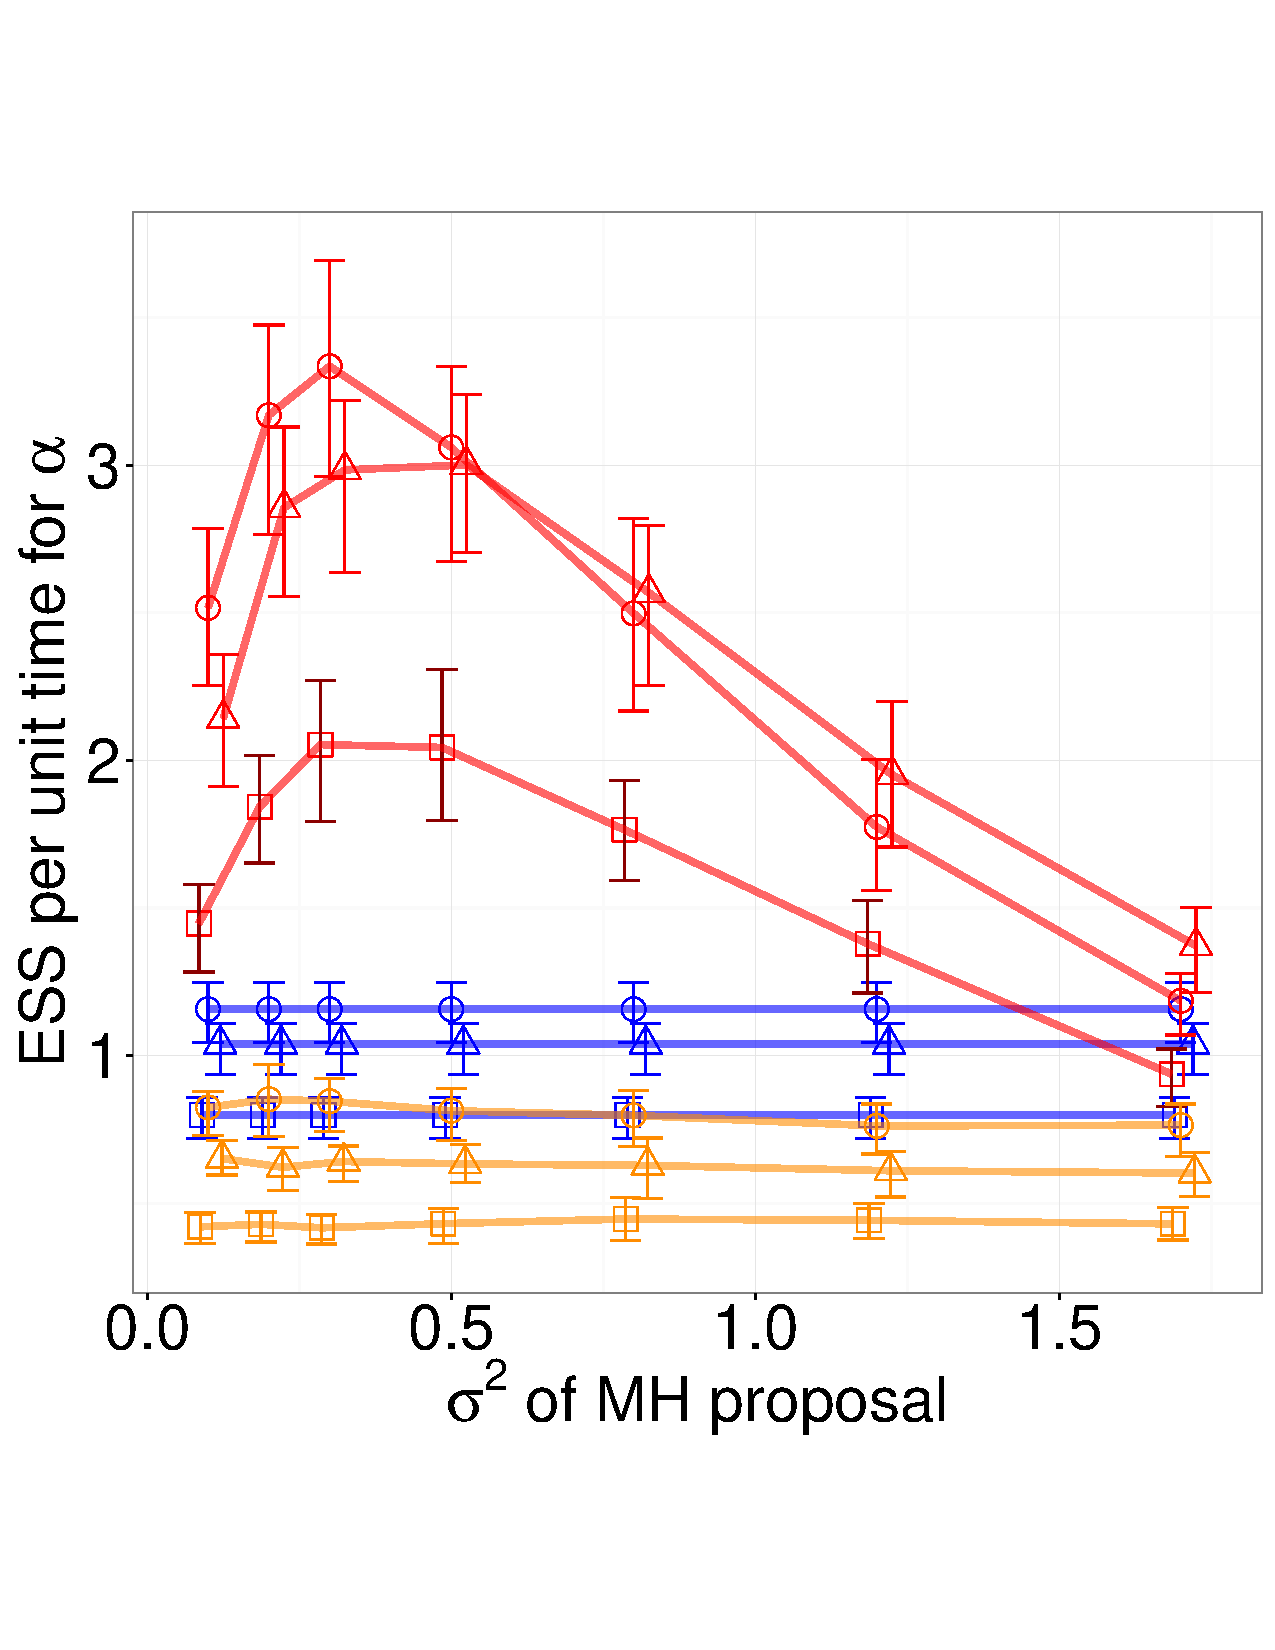
\includegraphics [width=0.42\textwidth, angle=0]{figs/pc_3_alpha.pdf}
    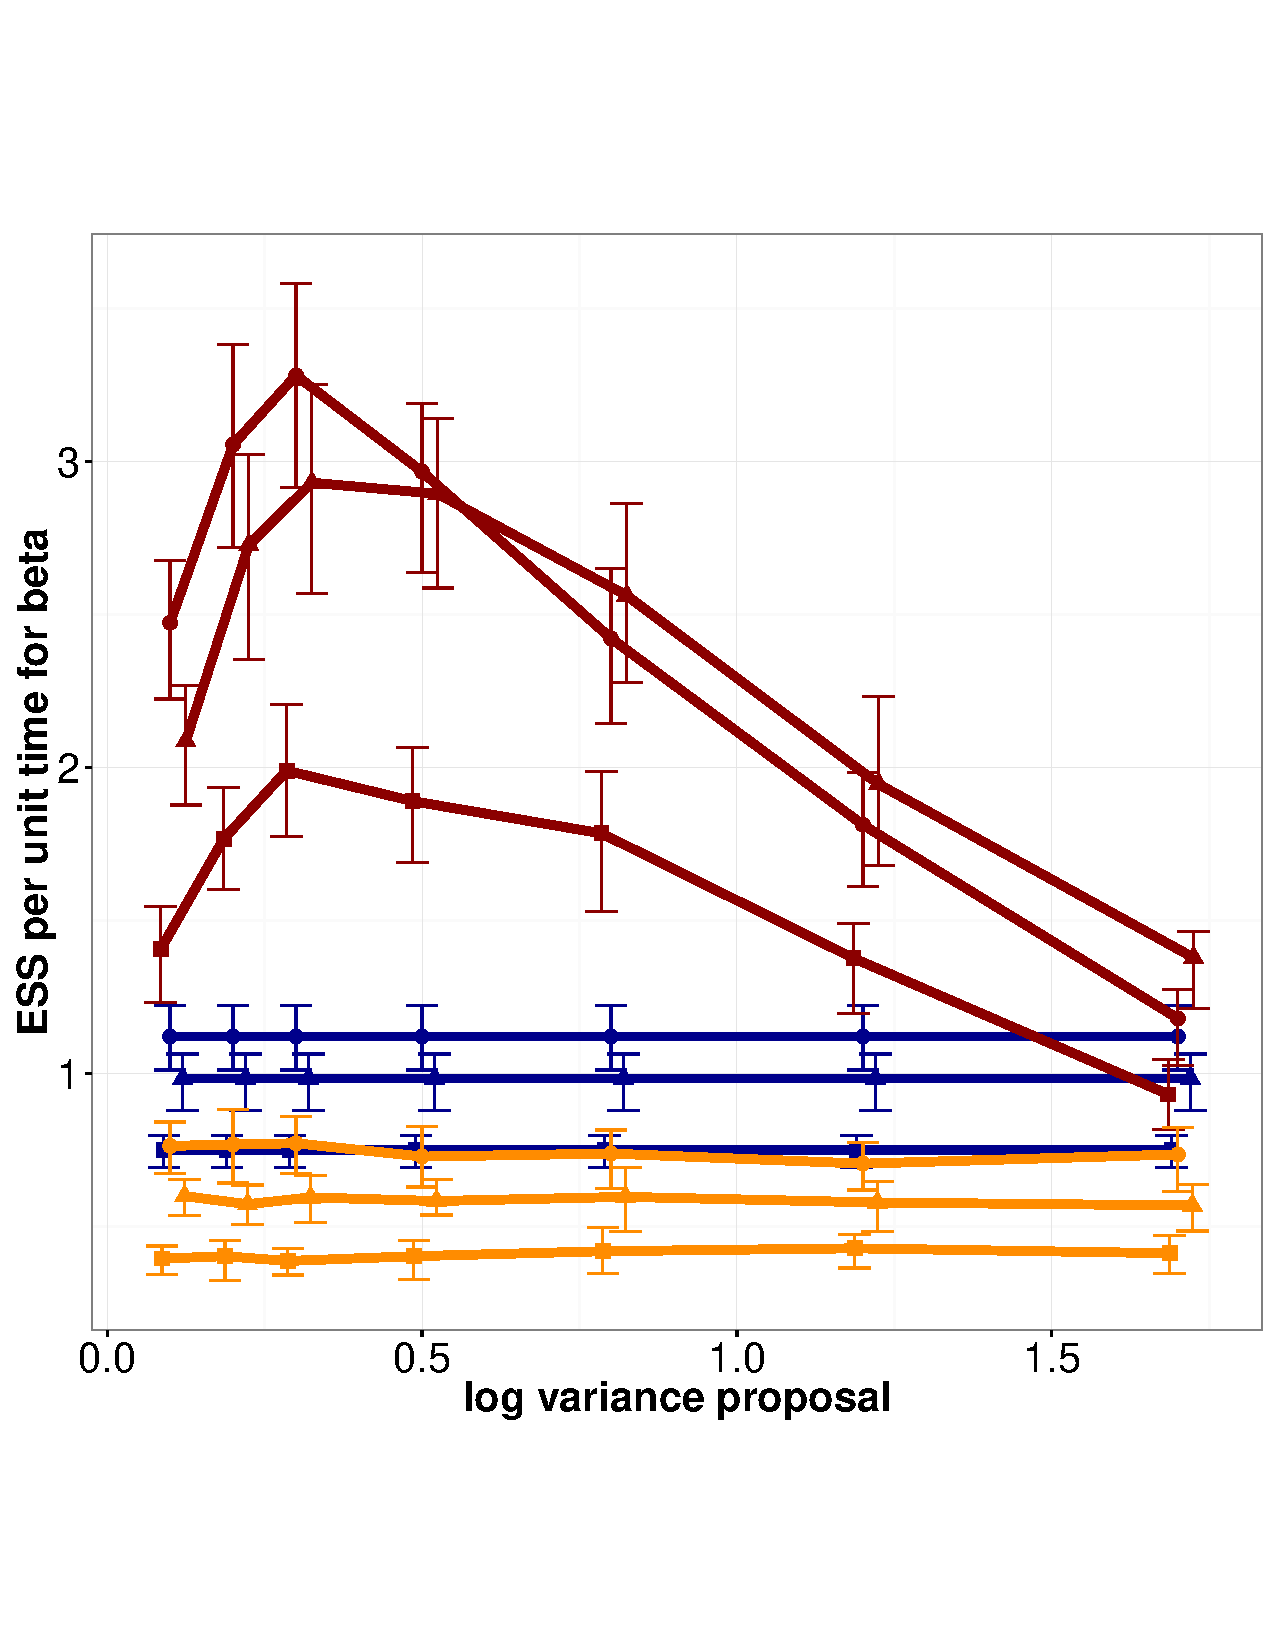
\includegraphics [width=0.42\textwidth, angle=0]{figs/pc_3_beta.pdf}
%    \vspace{-.81 in}
  \centering
    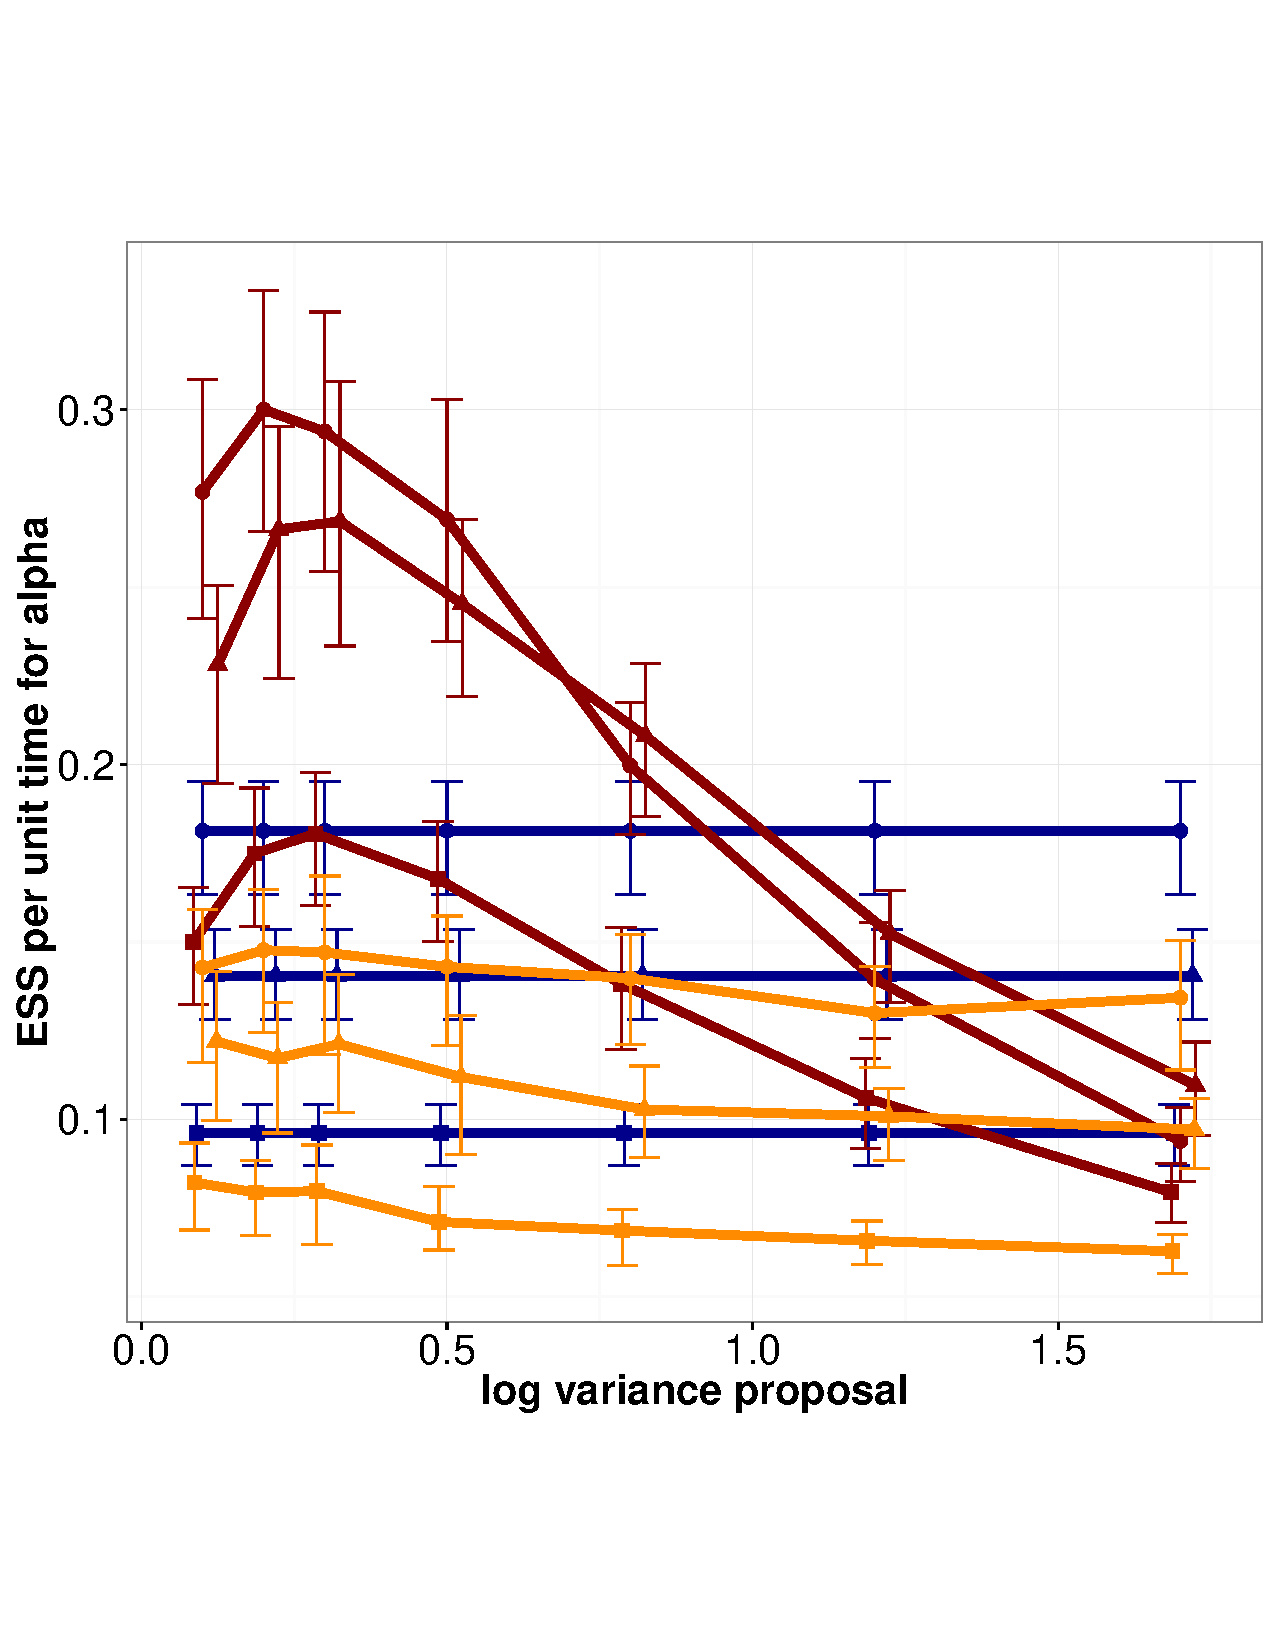
\includegraphics [width=0.42\textwidth, angle=0]{figs/pc_10_alpha.pdf}
    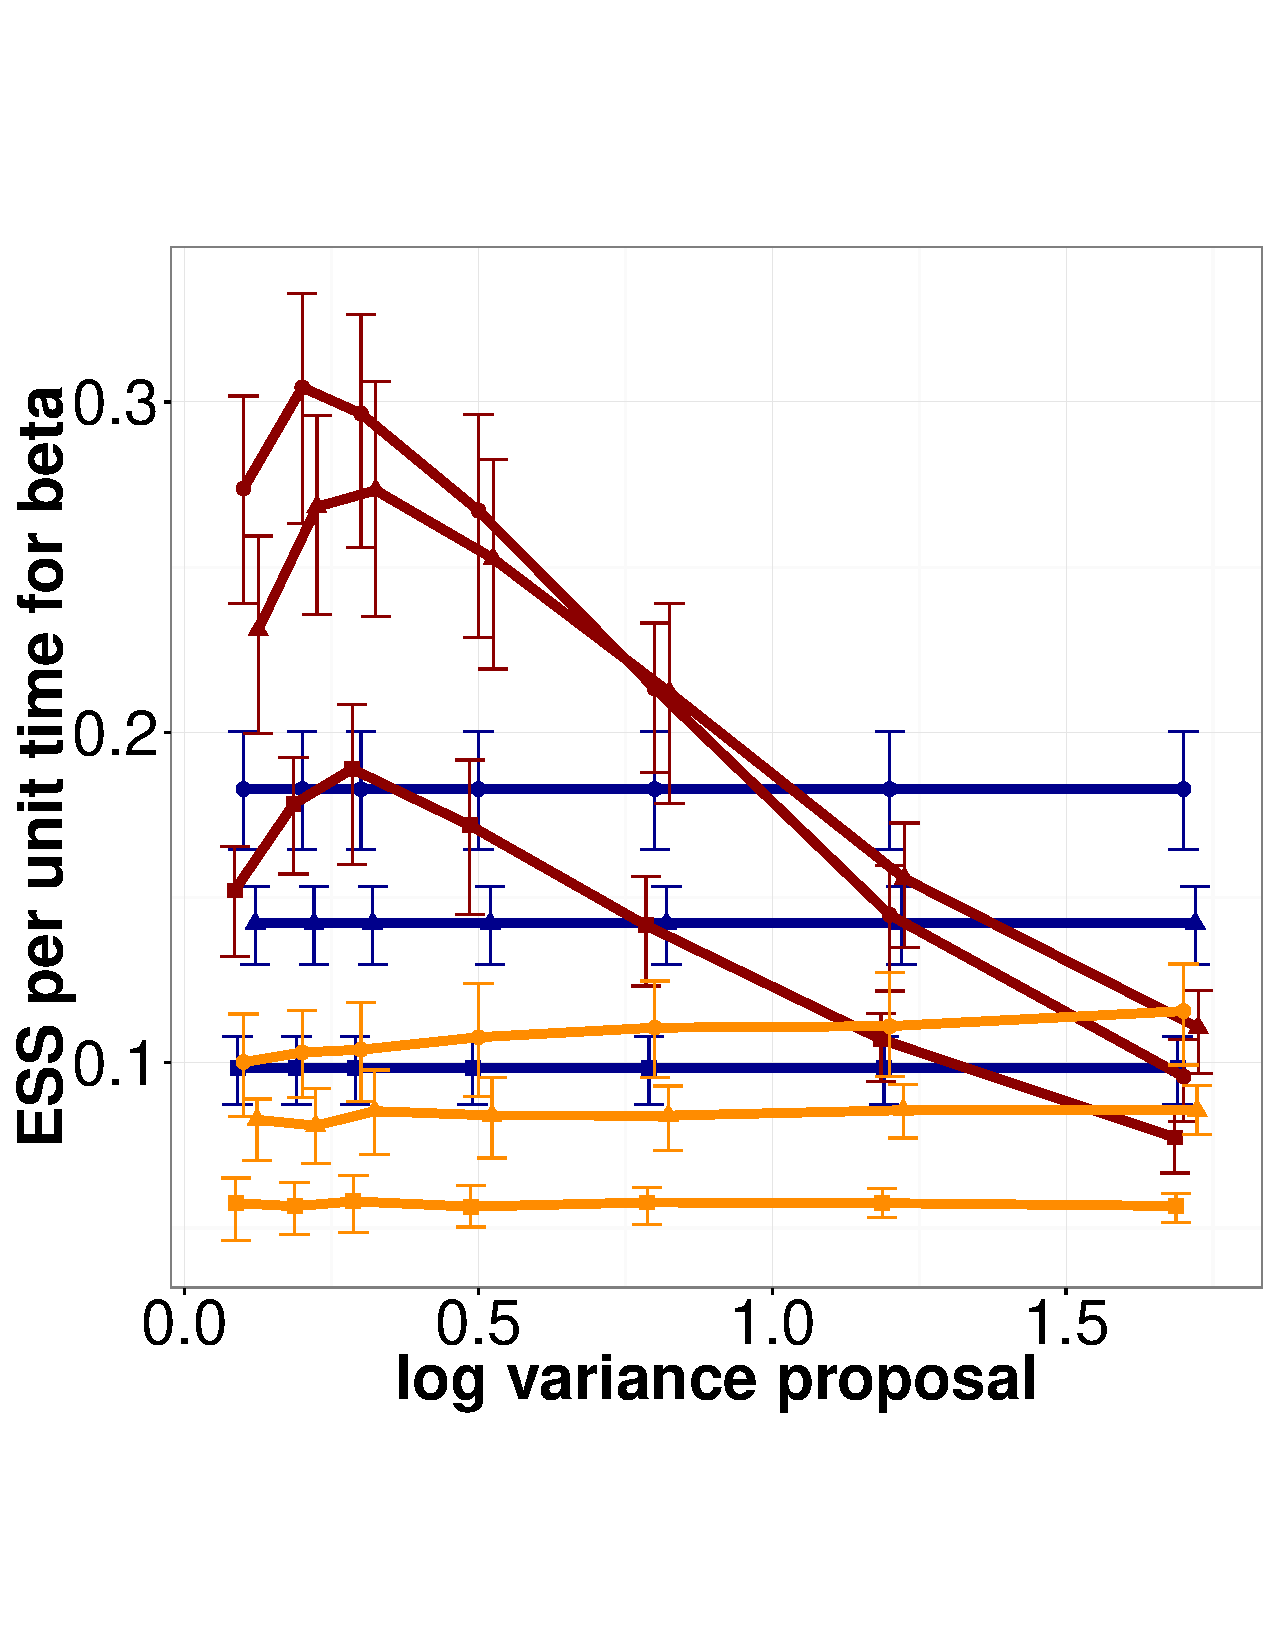
\includegraphics [width=0.42\textwidth, angle=0]{figs/pc_10_beta.pdf}
    \vspace{-.3 in}
  \end{minipage}
  \begin{minipage}[!hp]{0.04\linewidth}
  \end{minipage}
%  \begin{minipage}[!hp]{0.35\linewidth}
%    \vspace{-.3in}
    \caption{ESS/sec for the time-inhomogeneous immigration model, the top row 
      being dimension 3, and the bottom,
      dimension 10. The left column is for $\alpha$, and the 
    right is for $\beta$. Red, yellow and blue curves are the symmetrized MH,
  \naive\ MH, and Gibbs algorithm.}
     \label{fig:ESS_pc_10}
  %\end{minipage}
%    \vspace{-.2in}
  \end{figure}

  \begin{figure}[H]
%    \vspace{-.2in}
  \centering

  \begin{minipage}[!hp]{0.99\linewidth}
    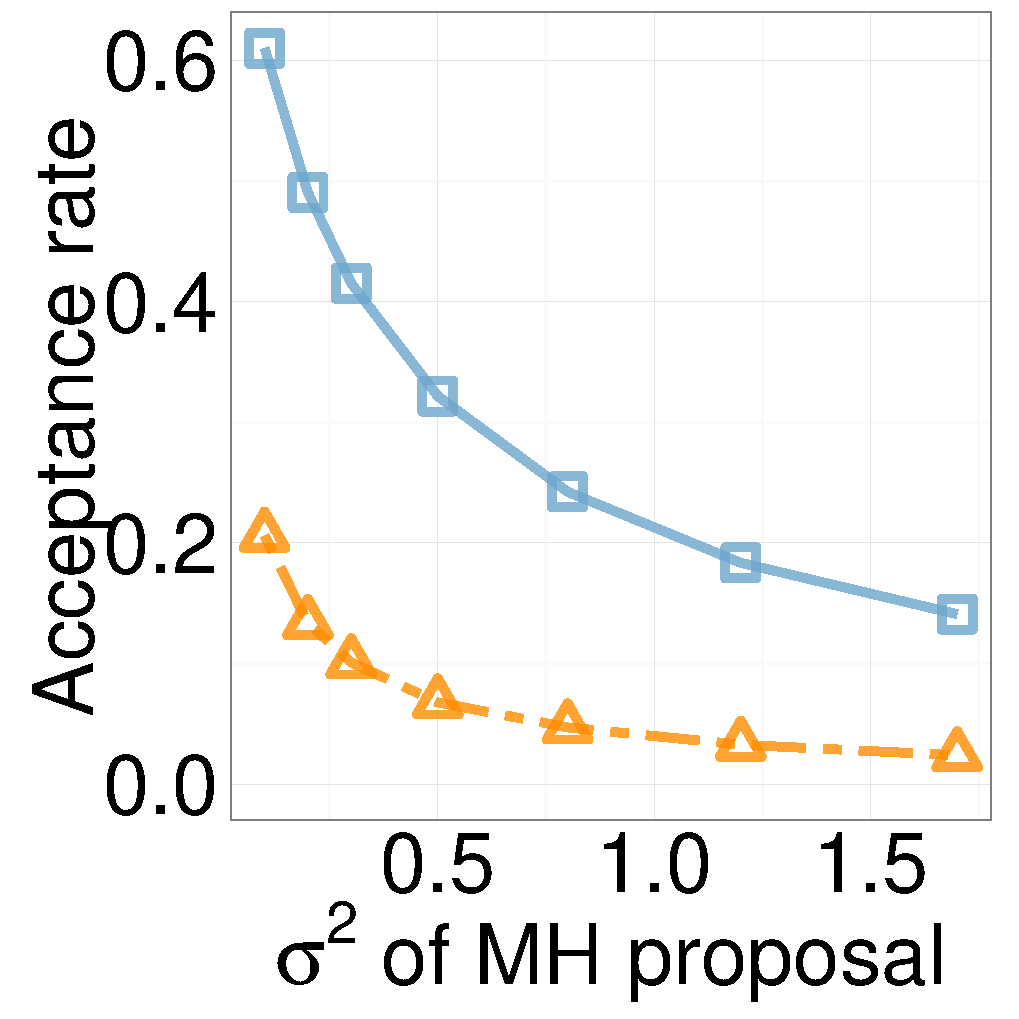
\includegraphics [width=0.40\textwidth, angle=0]{figs/acc/CQ_D3alpha_k2.pdf}
	\hspace{.5in}
    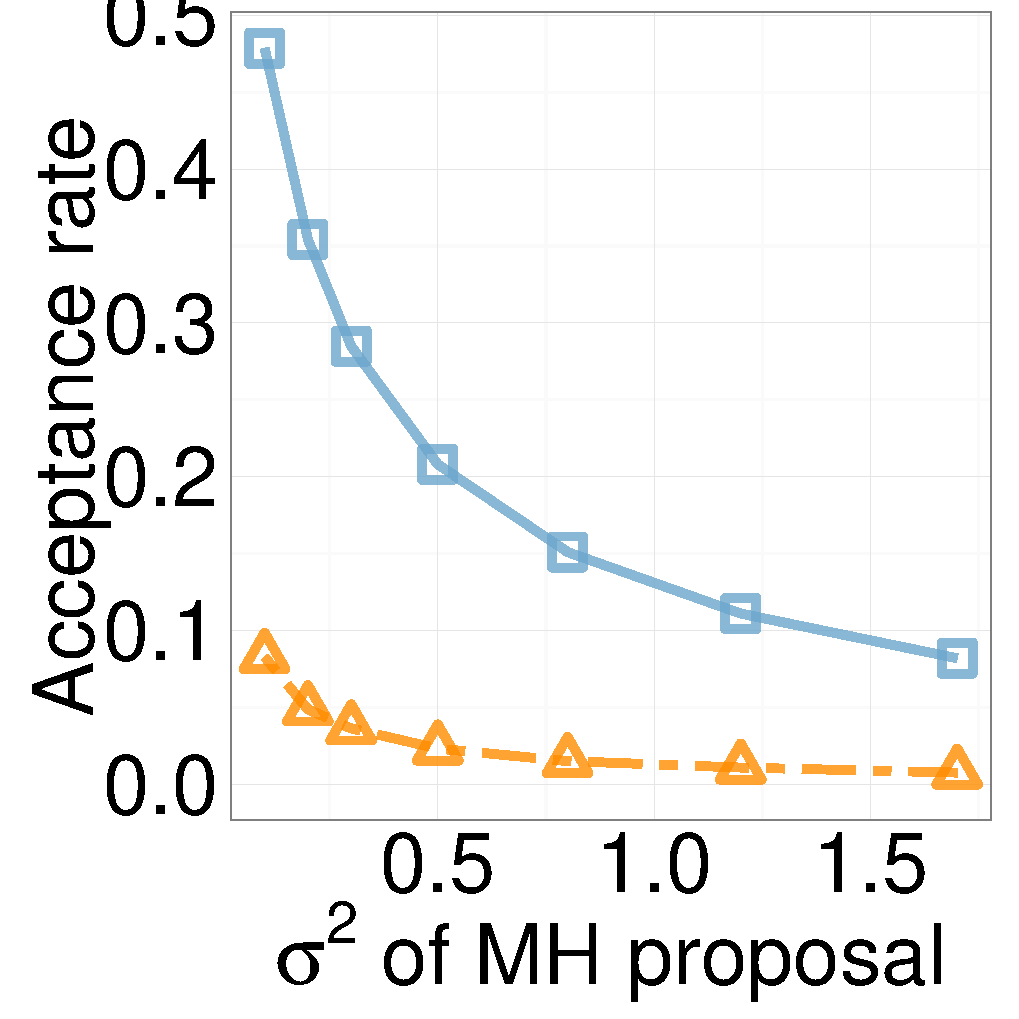
\includegraphics [width=0.40\textwidth, angle=0]{figs/acc/CQ_D10alpha_k2.pdf}
  \end{minipage}
%  \begin{minipage}[!hp]{0.99\linewidth}
    \caption{Acceptance Rate for $\alpha$ in the time-inhomogeneous immigration model, the left row being dimension 3, and the right,dimension 10.  Yellow and blue curves represent symmetrized MH,
 and \naive\ MH  algorithm. The multiplicative factor is $2$. }
     \label{fig:ACC_CQ}
%  \end{minipage}
  \end{figure}

  \begin{figure}[H]
%    \vspace{-.2in}
  \centering
%  \begin{minipage}[!hp]{0.99\linewidth}
 % \centering
  \begin{minipage}[!hp]{0.97\linewidth}
    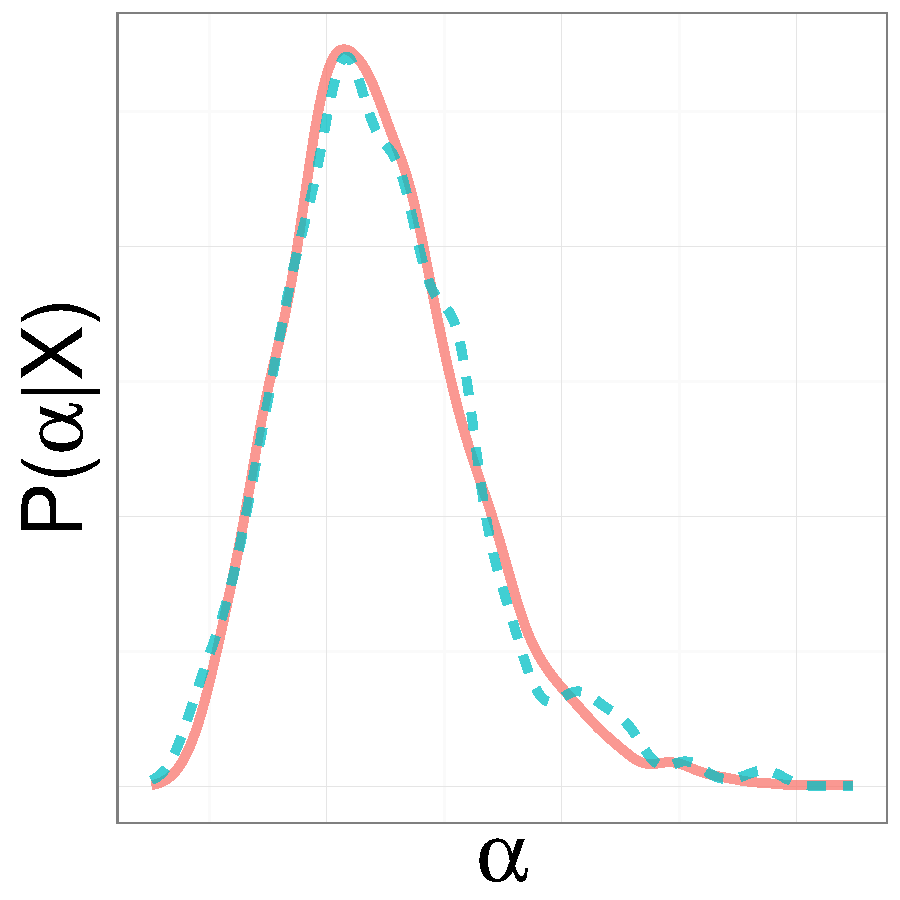
\includegraphics [width=0.30\textwidth, angle=0]{figs/QC_ks/qc_hist_4_03_10_.pdf}
    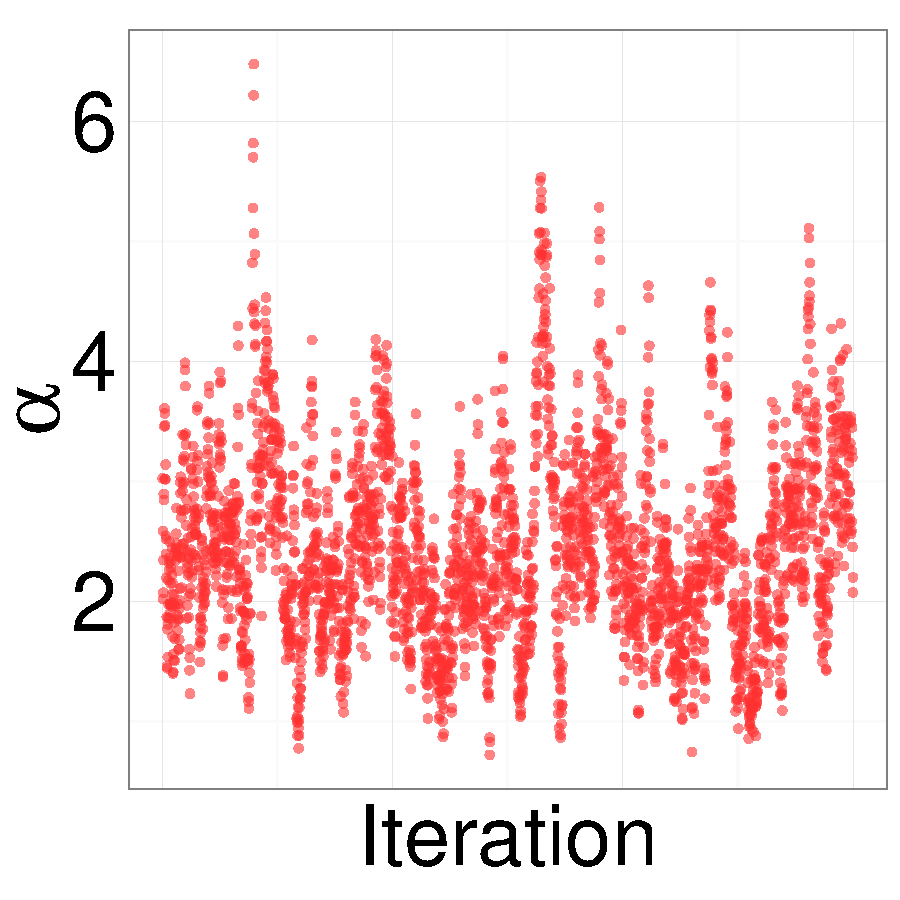
\includegraphics [width=0.30\textwidth, angle=0]{figs/QC_ks/qc_traceGBS_4_03_10_.pdf}
    \includegraphics [width=0.30\textwidth, angle=0]{figs/QC_ks/qc_traceMH_4_03_10_.pdf}
  \end{minipage}

%  \end{minipage}
%  \begin{minipage}[!hp]{0.99\linewidth}
    \caption{The left is histogram for the posterior samples($\alpha$) of the time-inhomogeneous immigration model with dimension 10, the red and blue curves are the Gibbs and symmetrized MH. The p value of the two sample-Kolmogorov Smirnov test is $ 0.7212$. The middle and the right are trace plots for the posterior samples of the time-inhomogeneous immigration model with dimension 10, the middle is for Gibbs and the right is for symmetrized MH}
     \label{fig:TRACE_CQ}
%  \end{minipage}
  \end{figure}

  \begin{figure}[H]
%    \vspace{-.2in}
  \centering
  \begin{minipage}[!hp]{0.99\linewidth}
    \includegraphics [width=0.40\textwidth, angle=0]{figs/QC_ks/qc_gbsacf_4_03_10_.pdf}
	\hspace{.5in}
    \includegraphics [width=0.40\textwidth, angle=0]{figs/QC_ks/qc_mhacf_4_03_10_.pdf}
  \end{minipage}

%  \begin{minipage}[!hp]{0.99\linewidth}
    \caption{ACFs for the posterior samples $\alpha$ of the time-inhomogeneous immigration model with dimension 10. The left is for Gibbs, and the right is for symmetrized MH.}
     \label{fig:ACF_CQ}
%  \end{minipage}
  \end{figure}

\textbf{A time-inhomogeneous immigration model:}
We extend the previous model to incorporate a known time-inhomogeneity. 
The arrival and death rates are no longer constant, and are instead given by
 %$$A_i(t) =: A_{i,i}(t) = -(\alpha + i\beta)w(t), \; \; i =0,1,...,N$$ 
$A_{i, i+1}(t) = \alpha w(t) \ (i =0,1,\cdots,N-1)$ respectively.
While it is not difficult to work with sophisticated choices of $w(t)$,
we limit ourselves to a simple piecewise-constant 
$w(t) = \left\lfloor \frac{t}{5} \right\rfloor$. Even such a simple
change in the original model can dramatically affect the performance
of the Gibbs sampler. \\
 The top row of figure~\ref{fig:ESS_pc_10} plots the ESS per unit time for the 
 parameters $\alpha$ (left) and $\beta$ (right) for the immigration model with 
 capacity $3$.  Now, the symmetrized MH algorithm is significantly 
 more efficient, comfortably outperforming all samplers (including the Gibbs 
 sampler) over a wide range of settings. %The Gibbs sampler slightly outperforms
 %the simple MH sampler, while particle MCMC is significantly worse (we have
% not included it).  
 Figure~\ref{fig:ESS_pc_10} shows performance for dimension
 $10$, once again the symmetrized MH-algorithm performans best over a 
 range of settings of the proposal variance. We note that increasing the
 dimensionality of the state space results in a more concentrated posterior,
 shifting the optimal setting of the proposal variance to smaller values.

  \subsection{Chi site data for Escherichia coli}~
  \begin{figure}%[b]
%    \vspace{-.2in}
  \centering
%  \begin{minipage}[!hp]{.32\linewidth}
%    \caption{ESS/sec for $(\alpha,\lambda_1)$ for the E.\ Coli data. The circles (in blue) are our 
%      proposed sampler as we vary the variance of the proposal distribution. 
 %     The straight line is the Gibbs sampler. }
  %   \label{fig:ECOLI}
%  \end{minipage}
  \begin{minipage}[!hp]{.01\linewidth}
    \hspace{.1in}
  \end{minipage}
%  \begin{minipage}[!hp]{.65\linewidth}
  \begin{minipage}[!hp]{.98\linewidth}
    \includegraphics [width=0.48\textwidth, angle=0]{figs/ECOLI_alpha.pdf}
    \includegraphics [width=0.48\textwidth, angle=0]{figs/ECOLI_l1.pdf}
%    \vspace{-.81 in}
 %   \includegraphics [width=0.24\textwidth, angle=0]{figs/ECOLI_beta.pdf}
 %  \includegraphics [width=0.24\textwidth, angle=0]{figs/ECOLI_l2.pdf}
%    \vspace{-.2in}
  \end{minipage}  
    \caption{ESS/sec for $(\alpha,\lambda_1)$ for the E.\ Coli data. The circles (in blue) are our 
      proposed sampler as we vary the variance of the proposal distribution. 
      The straight line is the Gibbs sampler. }
     \label{fig:ECOLI}

%   \vspace{-.3in}
  \end{figure}

  \begin{figure}[H]
%    \vspace{-.2in}
  \centering

  \begin{minipage}[!hp]{0.99\linewidth}
	\centering
    \includegraphics [width=0.50\textwidth, angle=0]{figs/acc/ecolialpha_k2.pdf}
  \end{minipage}
%  \begin{minipage}[!hp]{0.99\linewidth}
    \caption{Acceptance Rate of $\alpha$ generated by the symmetrized MH algorithm for the E.\ Coli data . The multiplicative factor is $2$. }
     \label{fig:ACC_ECOLI}
%  \end{minipage}
  \end{figure}

  \begin{figure}[H]
%    \vspace{-.2in}
  \centering
%  \begin{minipage}[!hp]{0.99\linewidth}
 % \centering
  \begin{minipage}[!hp]{0.97\linewidth}
    \includegraphics [width=0.30\textwidth, angle=0]{figs/ecoli_ks/ecoli_alphahist_31_3_0_.pdf}
    \includegraphics [width=0.30\textwidth, angle=0]{figs/ecoli_ks/ecoli_alphatraceGBS_31_3_0_.pdf}
    \includegraphics [width=0.30\textwidth, angle=0]{figs/ecoli_ks/ecoli_alphatraceMH_31_3_0_.pdf}
  \end{minipage}

%  \end{minipage}
%  \begin{minipage}[!hp]{0.99\linewidth}
    \caption{The left is histogram for the posterior samples($\alpha$) for the E.\ Coli data.The red and blue curves are the Gibbs and symmetrized MH. The p value of the two sample-Kolmogorov Smirnov test is $ 0.1641$. The middle and the right are trace plots for the posterior samples for the E.\ Coli data, the middle is for Gibbs and the right is for symmetrized MH}
     \label{fig:TRACE_ECOLI}
%  \end{minipage}
  \end{figure}

  \begin{figure}[H]
%    \vspace{-.2in}
  \centering
  \begin{minipage}[!hp]{0.99\linewidth}
    \includegraphics [width=0.40\textwidth, angle=0]{figs/ecoli_ks/ecoli_alphagbsacf_31_3_0_.pdf}
	\hspace{.5in}
    \includegraphics [width=0.40\textwidth, angle=0]{figs/ecoli_ks/ecoli_alphamhacf_31_3_0_.pdf}
  \end{minipage}

%  \begin{minipage}[!hp]{0.99\linewidth}
    \caption{ACFs for the posterior samples $\alpha$ for the E.\ Coli data The left is for Gibbs, and the right is for symmetrized MH.}
     \label{fig:ACF_ECOLI}
%  \end{minipage}
  \end{figure}

  \begin{figure}[H]
%    \vspace{-.2in}
  \centering
%  \begin{minipage}[!hp]{0.99\linewidth}
 % \centering
  \begin{minipage}[!hp]{0.97\linewidth}
    \includegraphics [width=0.30\textwidth, angle=0]{figs/ecoli_ks/ecoli_l1hist_31_3_0_.pdf}
    \includegraphics [width=0.30\textwidth, angle=0]{figs/ecoli_ks/ecoli_l1traceGBS_31_3_0_.pdf}
    \includegraphics [width=0.30\textwidth, angle=0]{figs/ecoli_ks/ecoli_l1traceMH_31_3_0_.pdf}
  \end{minipage}

%  \end{minipage}
%  \begin{minipage}[!hp]{0.99\linewidth}
    \caption{The left is histogram for the posterior samples($\lambda_1$) for the E.\ Coli data.The red and blue curves are the Gibbs and symmetrized MH. The p value of the two sample-Kolmogorov Smirnov test is $ 0.4658$. The middle and the right are trace plots for the posterior samples for the E.\ Coli data, the middle is for Gibbs and the right is for symmetrized MH}
     \label{fig:TRACE_ECOLI_l1}
%  \end{minipage}
  \end{figure}

  \begin{figure}[H]
%    \vspace{-.2in}
  \centering
  \begin{minipage}[!hp]{0.99\linewidth}
    \includegraphics [width=0.40\textwidth, angle=0]{figs/ecoli_ks/ecoli_l1gbsacf_31_3_0_.pdf}
	\hspace{.5in}
    \includegraphics [width=0.40\textwidth, angle=0]{figs/ecoli_ks/ecoli_l1mhacf_31_3_0_.pdf}
  \end{minipage}

%  \begin{minipage}[!hp]{0.99\linewidth}
    \caption{ACFs for the posterior samples $\lambda_1$ for the E.\ Coli data The left is for Gibbs, and the right is for symmetrized MH.}
     \label{fig:ACF_ECOLI_l1}
%  \end{minipage}
  \end{figure}

  We consider a dataset recording positions of a particular DNA motif 
  on the {\em E.\ coli} genome. Used in~\cite{FearnSher2006}, these 
  motifs consist of eight base pairs GCTGGTGG, and are called Chi sites.
  The rates of occurence of Chi sites provide information about genome 
  segmentation, allowing the identification of regions with high 
  mutation or recombination rates.
  %strands which are the inner and outer rings. The molecular mechanisms 
  %of DNA replication differ between the two half-strands and they are 
  %termed leading and lagging. The E. coli genome is 4639675 bases long and 
  %each half is 2319.838 kilobases long. 
  Following~\cite{FearnSher2006}, we wish to use this data to infer a 
  two-state piecewise-constant segmentation of the DNA strand. 
  We focus on Chi sites along the inner (lagging) strand of the 
  {\em E.\ coli} genome.  We place a 
  MJP prior over this segmentation, and indexing position along the 
  strand with $t$, we write this as $S(t)$ (\sout{$t \in [0,20]$ after rescaling 
  nucleotide indices} \boqian{$t \in [0,2319.838]$} ). To state $i \in 
  \{1,2\}$, we assign a rate $\lambda_i$, which together with $S(t)$, 
  defines a piecewise-constant rate function $\lambda_{S(t)}$. We model 
  the Chi-site positions as drawn from a Poisson process with rate 
  $\lambda_{S(t)}$, resulting in a {Markov-modulated Poisson 
  process}~\citep{scottmmpp03}. 
  MJP transitions from state $1$ to state $2$ have rate $\alpha$ while 
  transitions from state $2$ to state $1$ have rate $\beta$. We place 
  gamma priors are placed for the four model parameters; specifically, 
  we use Gamma$(2,2)$, Gamma$(2,3)$, Gamma$(3,2)$, Gamma$(1,2)$ for 
  $\alpha$, $\beta$, $\lambda_1$, $\lambda_2$ respectively.

  We use this setup to evaluate our symmetrized MH sampler along with 
  Gibbs sampling (other algorithms perform much worse). For our MH proposal distribution, we first 
  run \sout{$500$} \boqian{2000} iterations of Gibbs sampling to estimate the posterior 
  covariance of the vector $\theta = (\alpha,\beta,\lambda_1,\lambda_2)$, call this 
  $\Sigma_\theta$. Our MH proposal distribution is then $q(\nu|\theta) = 
  N(\nu|\theta, \kappa\Sigma_\theta)$ for different settings of 
  $\kappa$ (the typical choice is $\kappa = 1$)\boqian{, with the multiplicative factor $2$}. Figure~\ref{fig:ECOLI} 
  shows the results for parameters $(\alpha, \lambda_1)$, which are both 
  very similar. 
 % we include $(\lambda_1, \lambda_2)$ in the appendix. 
  We see that for the typical setting of $\kappa=1$, our 
  sampler ourperforms the Gibbs sampler, though Gibbs sampling does 
  outperform our method for large or small $\kappa$. This is because a) 
  large or small $\kappa$ mean the proposal variance is too large or too 
  small, and b) the Gibbs 
  conditionals over the parameters are conjugate for this model. Again,
  we expect the improvements our method offers to be more robust to the 
  proposal distribution for more complex models without such conditional 
  conjugacy.
% \begin{figure}%[b]
% \centering
% \begin{minipage}[!hp]{0.99\linewidth}
% \centering
%   \includegraphics [width=0.25\textwidth, angle=0]{figs/ECOLI_alpha.pdf}
%   \includegraphics [width=0.25\textwidth, angle=0]{figs/ECOLI_l1.pdf}
%  %   \includegraphics [width=0.24\textwidth, angle=0]{figs/ECOLI_beta.pdf}
%  %  \includegraphics [width=0.24\textwidth, angle=0]{figs/ECOLI_l2.pdf}
% %  \vspace{-.5in}
% \end{minipage}
%   \vspace{-.2in}
%   \caption{ESS/sec for the EColi data.}
%    \label{fig:ECOLI}
% \end{figure}

